

%%%%%%%%%%%%%%%%%%%%%%%%%%%%%%%%%%%%%%%%%%%%%%%%%%%%%%%%%%%%%%%%%%%%%%%%%%%%
%%%%%%%%%%%%%%%%%%%%%%%%%%%%%%%%%%%%%%%%%%%%%%%%%%%%%%%%%%%%%%%%%%%%%%%%%%%%
%%%%
%%%%                           OLD SNIPPETS
%%%%
%%%%%%%%%%%%%%%%%%%%%%%%%%%%%%%%%%%%%%%%%%%%%%%%%%%%%%%%%%%%%%%%%%%%%%%%%%%%
%%%%%%%%%%%%%%%%%%%%%%%%%%%%%%%%%%%%%%%%%%%%%%%%%%%%%%%%%%%%%%%%%%%%%%%%%%%%

\subsection{Flux units: vector quantities}

Also for vector quantities the physical dimension of the flux is
\begin{equation*}
  \frac{\textsf{quantity}}{\textsf{time}}
\end{equation*}
and its units will be the units of the quantity divided by seconds:
\begin{definition}{units of fluxes of the three vector quantities}
  \centering
  \begin{tabular*}{\linewidth}{@{\extracolsep{\fill}}lccc}
    \textbf{quantity}& momentum & ang. momentum
    \\[2\jot]
    \textbf{flux units}& \unit{N} & \unit{N\,m}
    \\[2\jot]
    \textbf{equivalent units}& \unit{kg\,m/s}  & \unit{kg\,m^2/s}
  \end{tabular*}
%  \caption{Units of scalar fluxes}
  \label{tab:fluxes_vector_units}
\end{definition}



\subsection{Flux units: scalar quantities}

Remember that the flux of a quantity is defined as an amount of that quantity \emph{per time lapse}. Therefore the physical dimension of the flux is
\begin{equation*}
  \frac{\textsf{quantity}}{\textsf{time}}
\end{equation*}
and its units will be the units of the quantity divided by seconds:
\begin{definition}{units of fluxes of the four scalar quantities}
  \centering
  \begin{tabular*}{\linewidth}{@{\extracolsep{\fill}}lccccc}
    \textbf{quantity}& matter & energy &
    \begin{minipage}{3em}
      \centering electric\\charge
    \end{minipage}
    &
        \begin{minipage}{4em}
      \centering magnetic\\field
    \end{minipage}
 & entropy
    \\[3\jot]
    \textbf{flux units}& \unit{mol/s} & \unit{J/s} & \unit{C/s} & \unit{Wb/s} & \unit{J/(K\cdot s)}
    \\[2\jot]
    \textbf{equivalent units}& \emph{watt} & \emph{ampere} \unit{A} & \unit{W} & \emph{volt} \unit{V} &
  \end{tabular*}
%  \caption{Units of scalar fluxes}
  \label{tab:fluxes_scalar_units}
\end{definition}

\bigskip

After our discussion about the peculiarity of fluxes it's quite easy to work with the fluxes of the four main scalar quantities: matter, electric charge, energy, entropy. Let us add some reminders and remarks about the fluxes of matter and energy.


\subsubsection{Matter flux}
\label{sec:matter_flux}

Remember that \emph{anti}matter \enquote{counts as \num{-1}} for calculating amounts of matter. If \qty{1}{mol} of positrons (anti-electrons) crosses a surface from left to right in \qty{1}{s}, the left-to-right flux of electrons equals \qty{-1}{mol/s} -- note the minus sign. The fact that antimatter is given special names can lead to ambiguities. For instance, if someone asks \enquote{what's the left-to-right flux of \emph{positrons}?}, maybe we should answer \enquote{\qty{1}{mol/s}}, since the question concerned specifically positrons. It's somewhat like asking \enquote{what's the flux of \emph{negative} electric charge?}. In these ambiguous situations it's best to add some explanatory words.

\subsubsection{Energy flux}
\label{sec:energy_flux}
We already mentioned that \autoref{sec:forms_energy}{energy flux can be categorized into different kinds}, depending on whether there are fluxes of other quantities through the same surface. We study the exact definitions and formulae later on. The total flux is given by the sum of all these kinds. For instance, through a horizontal surface we can have a downward energy flux of \qty{3}{J/s} as \emph{heat}, and a downward flux of \qty{-1}{J/s} as \emph{work}. The total downward flux is then \qty{2}{J/s}. The energy flux that you will calculate in the fourth exercise below is called \emph{energy convection}.




----

  We can also consider a \emph{temporal sequence} of control volumes, one for each instant of time. They can have positions, shapes, sizes that change smoothly from one time instant to the next. This sequence is often also called \enquote*{control volume} for short; but note the difference from the original meaning, which refers to one time instant only.


  The instantaneous movement and velocity of such a surface is important; therefore this region must, intuitively speaking, exist also an instant right before and right after the given time.

  \smallskip

  We can also consider a \emph{temporal sequence} of control surfaces, one for each instant of time. They can have positions, shapes, sizes that change smoothly from one time instant to the next. This sequence is often also called \enquote*{control surface} for short; but note the difference from the original meaning, which refers to only one time instant.

In the case of a control volume, movement does not matter: \emph{the volume content in a control volume does not depend on the instantaneous motion of the volume}. In fact we can even imagine a control volume that exists for just one time instant.

% 
\marginpar{\vspace{0\baselineskip}\centering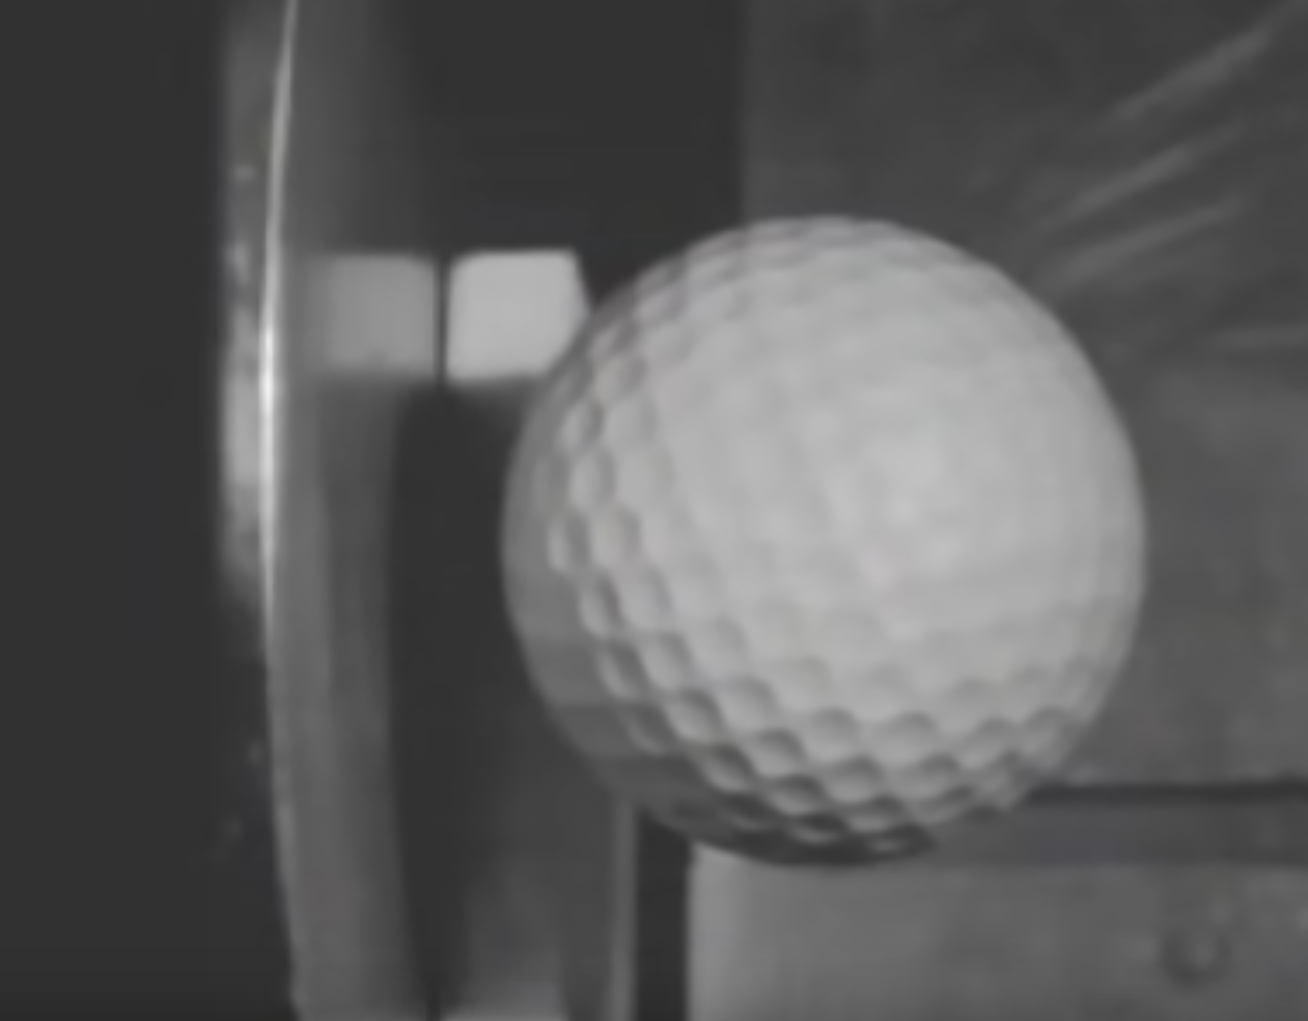
\includegraphics[width=\linewidth]{images/ball_wall.png}%
\\[\jot]\footnotesize\flushleftright\color{mpcolor}The golf ball is moving leftwards. Will it hit the metal surface? We don't know unless we know how the surface is moving.%
}%
In the case of a control surface the situation is different. The flux through a control surface \emph{depends also on the motion of the surface}. As a trivial example, consider a glass surface, and a person on one side of it, moving with a high velocity directed towards the surface. Will the person crash on the glass? We can't say for sure. The glass surface could be a glass wall in a building, which is not moving with respect to the person. In this case the person will likely crash on it. Or the glass surface could be the windscreen of a car, and the person could be the car's driver. In this case the person won't crash on the glass surface, because they're moving together with the same motion. Therefore we can't just imagine a surface that exists for one time instant: we need to imagine it at least for a very short time lapse, and be able to say how it's moving. If someone asks us what's the flux through a control surface at a given instant, but we are not told what's the motion of the surface, then the flux is unknown.




----

  of the quantity through the given surface. This measurement has the unit of the quantity divided by time. Remember that the flux through a surface depends on how that surface is moving.
  The \textbf{volume content} or \textbf{volume integral} is the amount of a quantity contained within a three-dimensional region, at a specific time instant. It has the same physical dimension as the quantity.

\begin{definition}{Volume content}
  The \textbf{volume content} or \textbf{volume integral} is the amount of a quantity contained within a three-dimensional region, at a specific time instant. It has the same physical dimension as the quantity.
\end{definition}



\smallskip

  Measurement~(2b) is called the \textbf{flux} of the quantity through the given surface. This measurement has the unit of the quantity divided by time. Remember that the flux through a surface depends on how that surface is moving.

  \smallskip

  Measurement~(3b) is called the \textbf{supply} or \textbf{source} of the quantity in the given volume. This measurement has the unit of the quantity divided by time. The supply can be \emph{negative}, in which case it means that the quantity is being destroyed.
\end{definition}


\begin{enumerate}[noitemsep]
\item[(1)] We can speak about the amount of quantity contained within a three-dimensional region, at a specific time instant.

  \smallskip

\item[(2a)] We can speak about the amount of quantity flowing through a two-dimensional surface during a time lapse\textellipsis
\item[(2b)] \textellipsis or alternatively we can speak about the amount of quantity flowing through a two-dimensional surface \emph{per time}, at a particular time instant.

  \smallskip

\item[(3a)] We can speak about the amount of quantity produced within a three-dimensional region during a time lapse\textellipsis
\item[(3b)] \textellipsis or alternatively we can speak about the amount of quantity being produced within a three-dimensional region \emph{per time}, at a particular time instant.
\end{enumerate}
Let's give definite names to these three measurements:
\begin{definition}{{Volume content, flux, supply}}
  Measurement~(1) is called the \textbf{volume content} or \textbf{volume integral} of the quantity. This measurement has the same unit as the quantity.

  \smallskip

  Measurement~(2b) is called the \textbf{flux} of the quantity through the given surface. This measurement has the unit of the quantity divided by time. Remember that the flux through a surface depends on how that surface is moving.

  \smallskip

  Measurement~(3b) is called the \textbf{supply} or \textbf{source} of the quantity in the given volume. This measurement has the unit of the quantity divided by time. The supply can be \emph{negative}, in which case it means that the quantity is being destroyed.
\end{definition}


----



\subsection{The difference between flux and supply}
\label{sec:supply}

When we speak of \emph{supply} in the technical sense of measurement~(3b) above, we mean that there is \emph{creation} (positive supply) or \emph{destruction} (negative supply) of some amount of quantity in a region of space, during a lapse of time. By \enquote{creation} we mean that there's an increase in the amount of quantity in the region, which cannot be accounted for by the amount that \emph{entered} the region. In a manner of speaking, some of that quantity \enquote{appears from nowhere}, or \enquote{disappears into nowhere}.

In some cases the creation or destruction of a quantity is accompanied by the simultaneous destruction or creation of another quantity: there is actually a transformation taking place. So if we take both quantities together there is no creation or destruction. For example, in a container we may have some amounts of oxygen and hydrogen disappearing, and some amount of water appearing. We know that it is because the \emph{atoms} of these three substances are recombining in different ways; they are not created or destroyed. Yet it's a fact that there is a decrease of oxygen and hydrogen \emph{molecules}: we can count them, and observe that their number diminishes with time, and not because they are exiting the container. The opposite is true for water molecules: we observe their number increases with time, and not because they are entering the container.

Therefore it does make sense to speak about, and to quantify, such increase or decrease of a quantity that occurs in a region of space during a lapse of time, which occurs not because the quantity is entering or leaving through the region's boundary. % We call the increase in the unit of time the \textbf{supply} or \textbf{source} of that quantity.
\begin{definition}{Supply}
  We call \textbf{supply} or \textbf{source} the amount of a quantity created (as opposed to flowed in) in a given volume in the unit of time.

  The supply can be \emph{negative}, in which case it means that the quantity is destroyed.

  The supply has the unit of the quantity divided by time.
\end{definition}

\medskip


----

\begin{definition}{Three basic measurements that can be made on the seven quantities}
  \begin{enumerate}[label=\arabic*.]\bfseries
  \item How much of this quantity is contained in a particular three-dimensional region of space at a particular time instant?

  \item How much of this quantity flows through a particular two-dimensional surface during a particular time lapse?

  \item How much of this quantity is produced in a particular three-dimensional region of space during a particular time lapse?
  \end{enumerate}
\end{definition}
%
\marginpar{\vspace{-11\baselineskip}\centering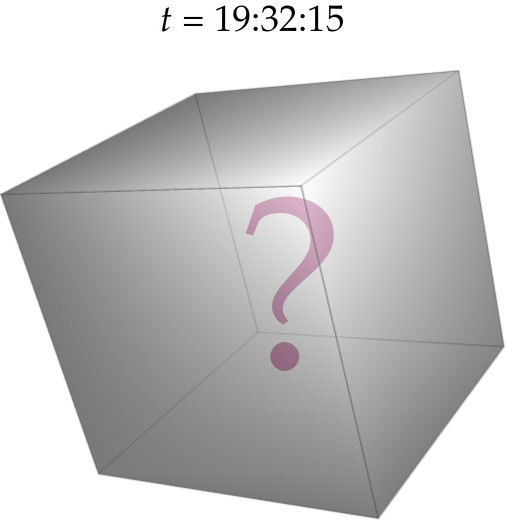
\includegraphics[width=\linewidth]{images/howmuch_volume.jpg}%
\\[\jot]\footnotesize\flushleftright\color{mpcolor}%
For six main quantities we can ask: how much of it is in a given volume, at a given time?

\mbox{}
\\[2\baselineskip]\centering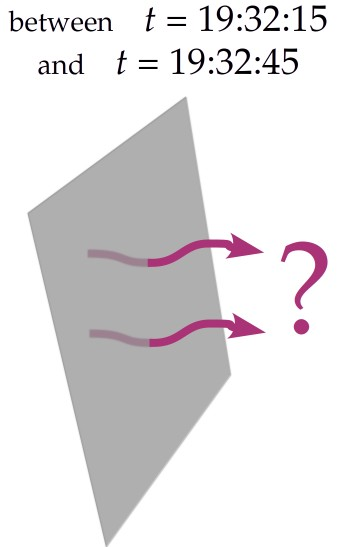
\includegraphics[width=0.7\linewidth]{images/howmuch_surface.jpg}%
\\[\jot]\footnotesize\flushleftright\color{mpcolor}%
For six main quantities we can ask: how much of it is flowing through a given surface, during a given time lapse?%
}%
We can ask these questions of any region of space, any time instant, and any time lapse. The surface in the second question can be moving and deforming. The results of the three measurements above are numbers (positive or negative) for scalar quantities; and vectors for vector quantities. In the case of magnetic flux we can ask the three questions above in 2 and 1 dimensions, rather than in 3 and 2 dimensions, as we shall see in \chap~\ref{cha:cons_magneticflux}.
% This number depends only on the chosen region, surfaces, and times.

The second and third questions, about the flow through a surface and the production in a region, can also be asked in a slightly different way. We can consider a very short lapse of time, and divide the net flow and the net production by that time lapse. This way we have an alternative form of the second and third measurements, as flow or production divided by time. They are called the \textbf{flux} and the \textbf{supply} of the quantity:
\begin{definition}{Flux of a quantity through a surface}
  \begin{enumerate}[label=\arabic*.]\bfseries
  \item[2b.] How much of this quantity is flowing through a particular two-dimensional surface, per time, at a particular time instant?
  \end{enumerate}
\end{definition}

\begin{definition}{Supply of a quantity in a region}
  \begin{enumerate}[label=\arabic*.]\bfseries
  \item[3b.] How much of this quantity is being produced through a particular three-dimensional region of space, per time, at a particular time instant?
  \end{enumerate}
\end{definition}

\medskip

The second property common to all seven quantities tells how the measurements above combine for several regions of space and several surfaces:
\begin{definition}{Extensivity or additivity,label={def:extensivity}}
\begin{enumerate}[label=\arabic*.]\bfseries
  \item[3.]  If we consider two or more non-overlapping volumes, the amount of quantity in the total volume is equal to the sum of the amounts in the individual volumes.

    If we consider two or more non-overlapping surfaces, the amount of quantity flowing through the total surface is equal to the sum of the amounts flowing through the individual surfaces.
  \end{enumerate}

We say that each of the seven quantities is an \textbf{extensive} or \textbf{additive} quantity.
\end{definition}

% We shall later see that analogous properties hold for the magnetic flux, the only difference being that instead of holding in 3 and 2 dimensions, they hold in 2 and 1 dimensions.




----

Given a coordinate time it is possible to define an alternative distance, which we can call \textbf{spatial coordinate distance} or just \enquote*{coordinate distance} for short. It is the length of the path joining you and the object at coordinate time $t$ for both; all points of the path are also understood to be at coordinate time $t$ as well. The path should be a \emph{straight line} (geodesic) between you and the object. As mentioned before, there may be several geodesics connecting you and the object at coordinate time $t$. This fact may lead to some complications. For instance there may be different paths having shortest distance; therefore saying \enquote{the path of shortest distance} may be ambiguous.

Coordinate distance has two advantages. First, it does \emph{not} depend on the relative motion between you and the object. Second, it can also be defined for very faraway objects. It is often difficult to measure directly, however, and often can only be extrapolated.



These problems are all bypassed by using a \textbf{spatial coordinate system}, or \enquote*{coordinate system} for short. A coordinate system is the assignment, by agreement, of three numerical labels to every point in a given region of space, \emph{for each coordinate time}. We use symbols for these labels, such as $(x,y,z)$ or $(r, \theta,\phi)$ or others. The values of these labels are thus the same for all observers. Often these labels have physical meaning, such as the distance from some event as measured by a specific observer, but they don't need to. In situations where only two or just one dimension are relevant, we can just use two or one spatial coordinates.



We take a metallic spring (or a rubber band) and attach two identical clocks at either extremity, let's call the extremities A and B. We contract the spring so that the two clocks touch; and right when they touch, we synchronize them so that they show the same time. The spring is then released; its two extremities move; the spring alternately stretches and contract while moving.

Later on we observe the spring while its two end happen, for an instant, to touch again and to be very close to us. As the two ends A and B touch, we can agree that the length of the spring is zero. But \emph{at what time} is it zero? Our clock shows time $t_{\textrm{us}}$, the clock at end A of the spring shows time $t_{A}$, and the clock at end B shows time $t_{B}$. These three times will generally be different. So \emph{for us} the spring has zero length at time $t_{\textrm{us}}$. For end A, the length is zero at the different time $t_{A}$. And for end B, the length is zero at a yet different time $t_{B}$. Clearly we cannot specify an absolute time at which the spring has zero length: we can only specify it relative to some moving clock.

The situation is even more complicated if we ask \enquote{what is the length of the spring at time $t$?}. First of all we must specify \emph{whose} time $t$. Let's say it's the time shown by our clock.


The time elapsed for us, for one spring end, and for the other end will generally be different.



Think of a metallic spring or a rubber band that is alternately stretching and contracting, while moving. The question \enquote{what is the length of the metallic spring \emph{right now}?} does not make sense, because there is no universal \enquote*{now}. Imagine of attaching a clock to either end of the metallic spring


We could attach one clock at either end of the metallic spring, but the synchronization of these two clocks would be arbitrary, and the time elapsed for each would depend on its motion in spacetime. The synchronization 

Traditionally when we speak of the distance of a moving object at a given time, we mean the distance at the same instant of time, measured on a straight line. But we have seen that it does not make sense for us to ask \enquote{what is the time for the object, right now?}; and moreover, spacetime is curved. Owing to the path-dependence of time and to curvature, we can define and measure several \enquote*{distances}, which are \emph{not} equivalent to one another.



%%%% Time space begin

Note therefore the following curious situation. In setting up a time to meet a friend, you don't need to worry about the discrepancies between your and your friend's proper times: if your friend walks \qty{1000}{m} away from you and then immediately back to you, at \qty{1}{m/s}, then the time elapsed for you will be \qty{1000}{s} (around \qty{17}{min}), but the time elapsed for your friend will be \qty{999.999999999999994437}{s}. That's a difference of less than \qty{e-14}{s}, clearly negligible for the two of you, so you don't need to worry with General Relativity formulae in setting up your meeting time. Yet, if you set up a meeting place via GPS, then the true nature of time and General Relativity formulae become important: if they were not accounted for, you and your friend might end up off your meeting place by \qty{100}{m}.
% In most everyday situations for us, who live on or nearby Earth's surface and move at speeds much smaller than $\yc$ with respect to one another, the discrepancies between our proper times are so small that they cannot be measured with ordinary clocks or with our internal clocks. Consider a person walking \qty{10}{m} away from you and then immediately walking back to you, at \qty{1}{m/s}. The time elapsed for you will be \qty{20}{s}, but for that person will be \qty{19.999999999999999889}{s}, a difference of \qty{e-16}{s}, which is the error of an atomic clock. %%***add ref
% If human beings will still exist in some decades or centuries, in space travel they will have to deal with large proper-time discrepancies also in everyday life.

Time lapse or duration has SI dimension \enquote*{\textsf{time}}, and we shall usually measure it using the unit \emph{second}, symbol \enquote*{$\unit{s}$}.

% *** add short explanation of second


\subsection{Coordinate time}
\label{sec:coord_time}

The fact that the time elapsed for you can be different from that elapsed for a satellite can therefore make it difficult to coordinate activities and to operate some technologies.

But luckily there's a way to bypass proper-time discrepancies. Instead of referring to my proper time or to your proper time, we can agree on assigning a somewhat arbitrary numerical time label to every event: this is called a \textbf{coordinate time}.

\medskip

Coordinate time is generally different from the proper times measured by different observers. It can nevertheless be used for \enquote{doing physics}, and it is the time we shall most often use in our equations. The coordinate time commonly used for Earth-physics purposes is \furl{https://www.nist.gov/pml/time-and-frequency-division/time-realization/utcnist-time-scale-0/}{Universal Coordinated Time UTC}, or the \furl{https://gssc.esa.int/navipedia/index.php?title=Atomic_Time}{International Atomic Time TAI} for astronomy purposes:
%\autocites[]{icwg1983_r2022}
\begin{quote}\footnotesize
  International Atomic Time (TAI) is based on more than 250 atomic clocks distributed worldwide that provide its stability, whereas a small number of primary frequency standards provide its accuracy. Universal Coordinated Time, which is the basis of all legal time scales, is derived from TAI. To allow the construction of TAI and the general dissemination of time, clocks separated by thousands of kilometres must be compared and synchronized. \textelp{} The achieved performances of atomic clocks and time transfer techniques imply that the definition of time scales and the clock comparison procedures must be considered within the framework of General Relativity. \sourceatright{\parencites{petitetal2005}}
%\mbox{}\hfill (\cites{petitetal2005})
\end{quote}
% \begin{figure}[h!]\footnotesize\centering%
% 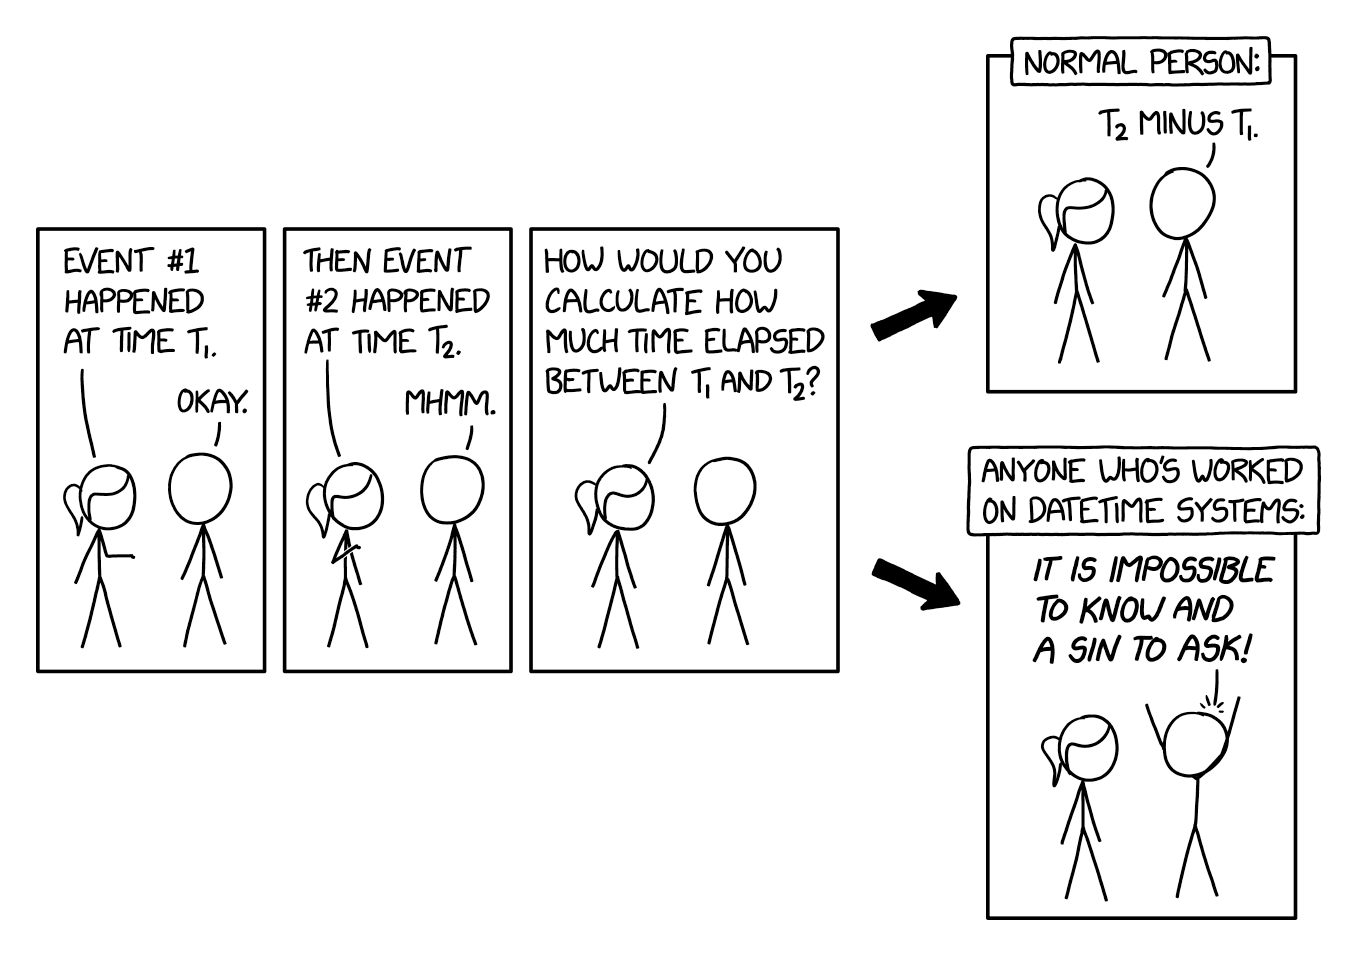
\includegraphics[align=t,width=0.75\linewidth]{images/datetime_2x.png}
% \\%
% \url{https://xkcd.com/2867}
% \end{figure}
UTC and TAI have the same time lapse, but UTC differ by irregular readjustments of its \enquote{zero}, the \furl{https://webtai.bipm.org/ftp/pub/tai/Circular-T/cirthtm/cirt.442.html}{leap seconds}.

The clock on your phone, and on devices synchronized via internet, shows UTC, not your proper time. An observer on Earth at \qty{0}{m} over sea level, and not moving, measures a proper-time lapse equal to UTC or TAI (besides small variations coming from the irregularity and internal motions of the Earth). But observers at other altitudes and observers moving with respect to Earth's surface can measure that their proper-times lapses are slightly different from UTC and TAI.

\medskip

In applications related to interplanetary spacecraft navigation and cosmological observations, the Barycentric Coordinate Time TCB is used. Its time lapse is slightly faster than the one of UTC: for each second that passes in UTC, \qty{1.0000000148}{s} pass in TCB on average. Two coordinate times to be used around an on the Moon, \furl{https://doi.org/10.1103/Physics.17.140}{Lunar Coordinate Time TCL} and Lunar Time LT, are on the making in the year 2025. Lunar Time will lapse faster by \qty{5.6e-5}{s} per day compared to our UTC. The establishment of all these kinds of coordinate times shows how important the difference between coordinate and proper time is for our current technology.

\medskip

When we use coordinate time, some important physics formulae turn out to be the same no matter whether we use General Relativity or an approximate theory such as Newtonian Mechanics. Thanks to this fact, for the most part of these notes we will not need to deal with proper-time details. But it is important for you to keep in mind how time really works, and the small time discrepancies that exist and occur all the time along your \emph{worldline}.



\begin{exercise}[label={ex:clocks}]
  Consider two clocks: one at rest on the Earth's surface, at a distance $\color{green}r_{\text{e}}$ from the Earth's centre; the other on a GPS satellite or, say, on the \furl{https://www.nasa.gov/international-space-station/}{International Space Station}, right above the first clock, at a distance $\color{red}r_{\text{s}}$ from the Earth's centre. An observer by the clock on Earth measuring a time lapse $\Dt_{\text{e}}$ will see that the clock on the satellite has run for a time lapse $\Dt_{\text{s}}$. The relation between two time lapses is approximately given by
\sidepar{\centering%
  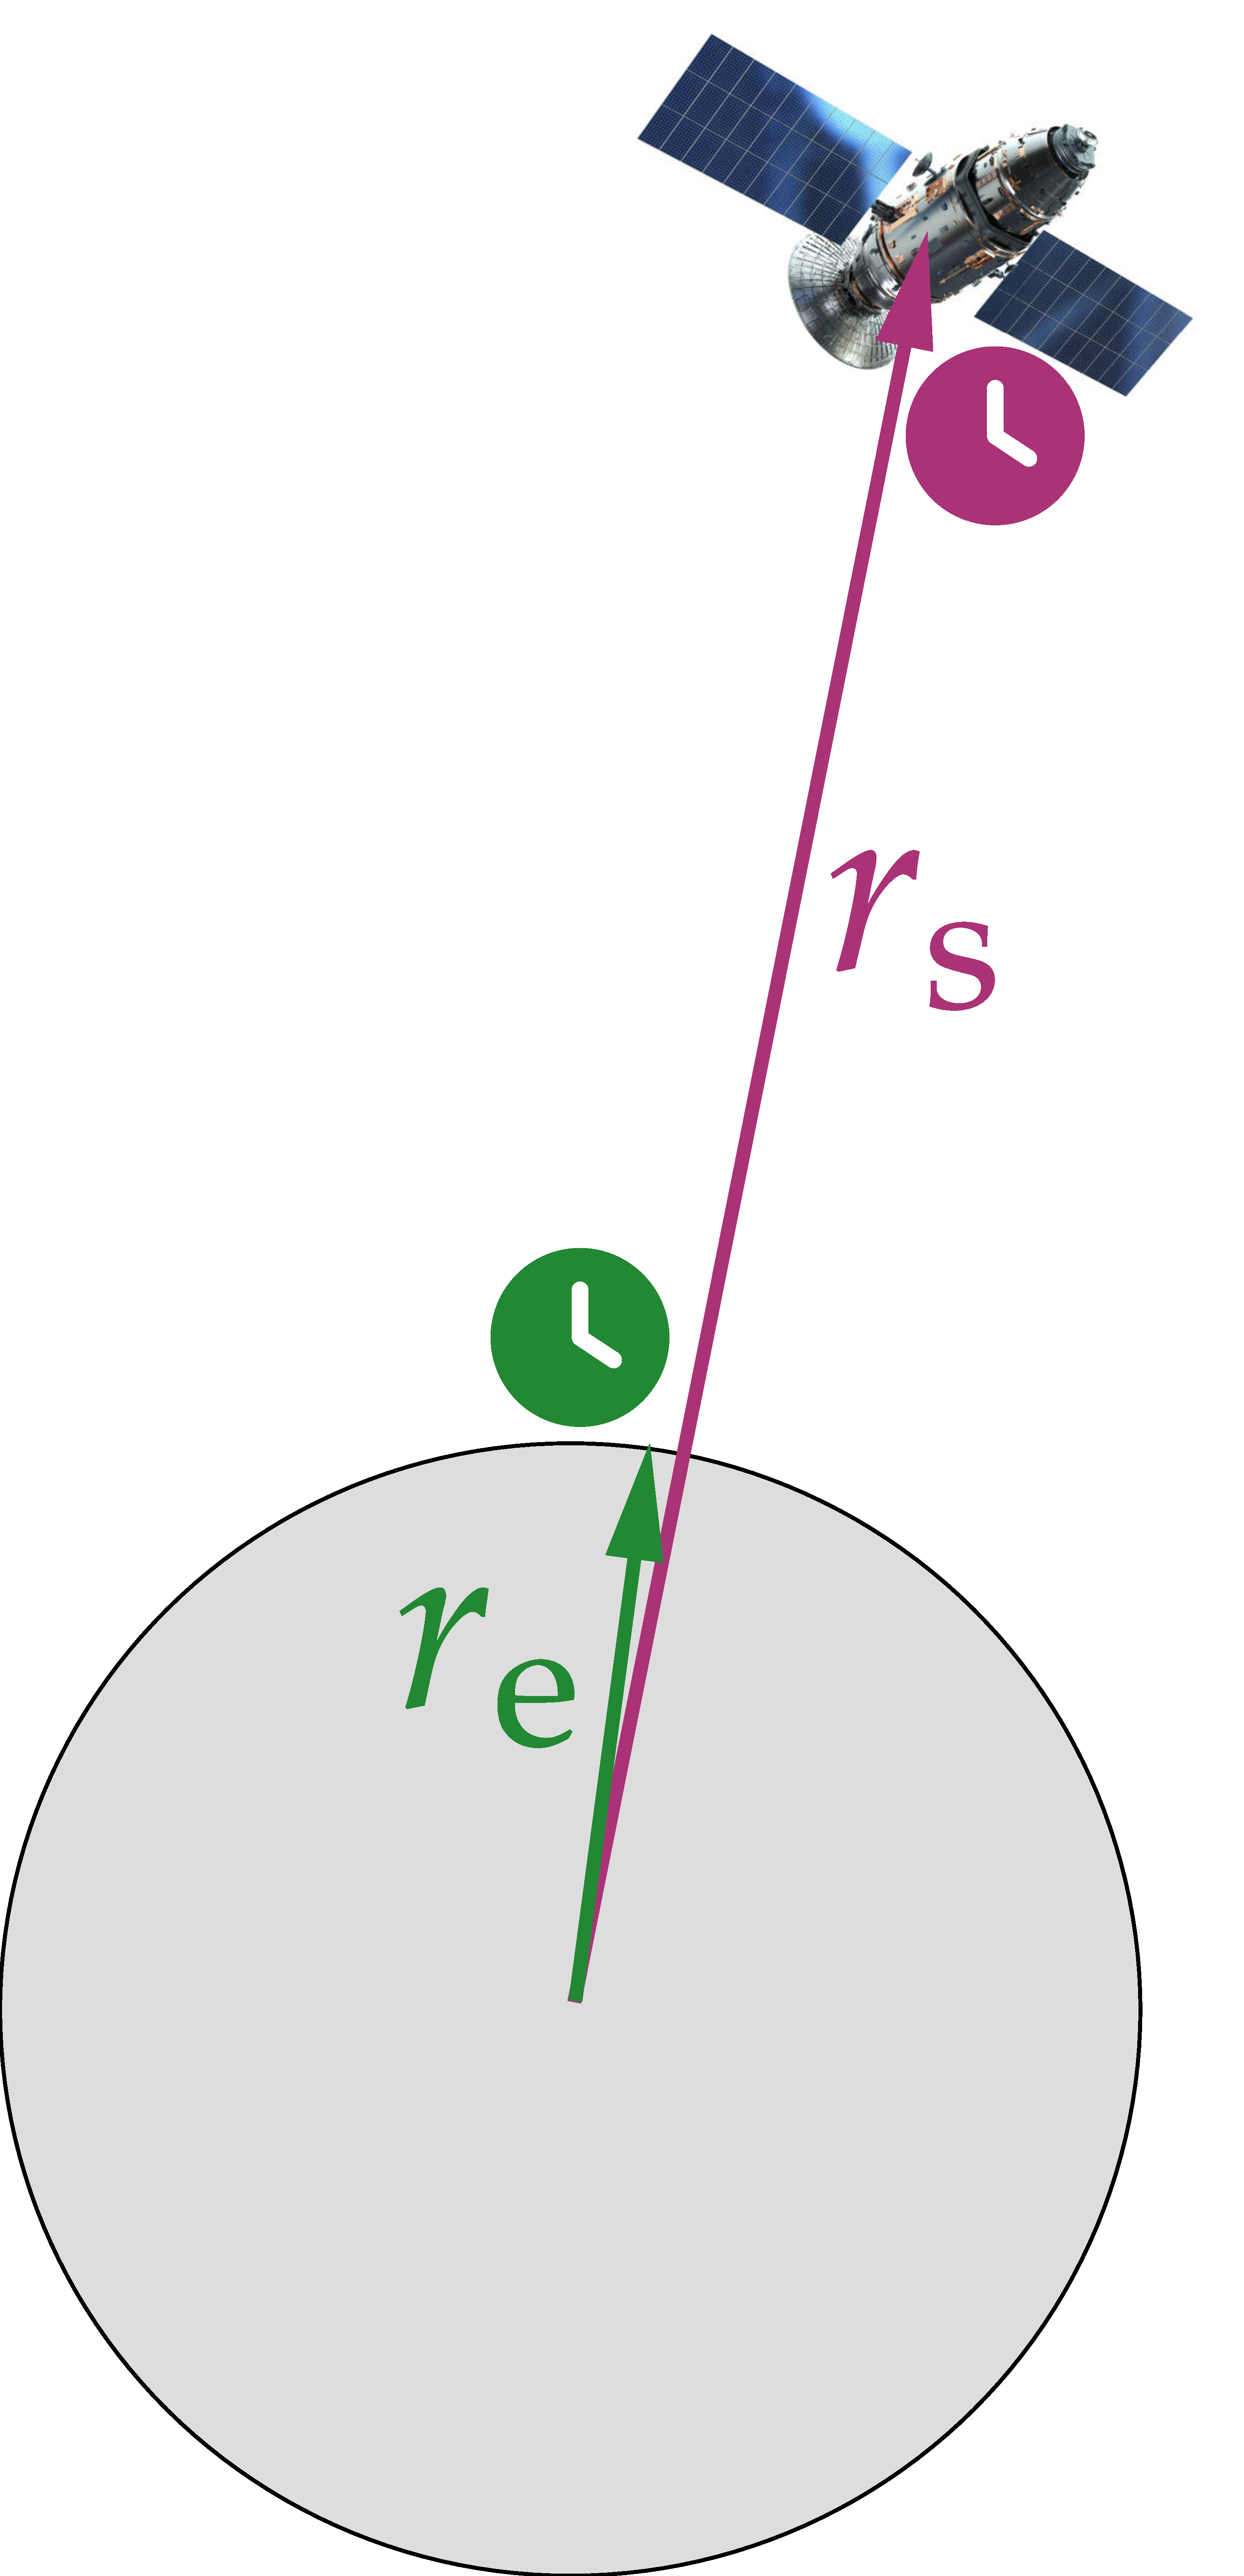
\includegraphics[align=t,width=0.75\linewidth]{images/re_rs.pdf}
}
\begin{equation*}
  \frac{\Dt_{\text{s}}}{\Dt_{\text{e}}} =
  \frac{
    \sqrt{1-2\frac{G}{c^{2}}\frac{M}{r_{s}}}
  }{
    \sqrt{1-2\frac{G}{c^{2}}\frac{M}{r_{e}}}
  }
\end{equation*}
where $G\approx\qty{6.7e-11}{m^{3}/(kg.s^{2})}$, $c=\qty{3.0e8}{m/s}$, and the Earth's mass $M=\qty{6.0e24}{kg}$.

\begin{enumerate}[exerc]
\item\label{item:gps_clock} Take the case of a GPS satellite, with $r_{\text{e}}=\qty{6.4e6}{m}$ and $r_{\text{s}}=\qty{2.6e7}{m}$ (\furl{https://www.nasa.gov/directorates/somd/space-communications-navigation-program/gps/}{NASA data}). If you, on the ground, measure a time lapse of $\Dt_{\text{e}}=\qty{10}{years}$, what's the difference, in seconds, with the time lapse $\Dt_{\text{s}}$ you see on the satellite?

\item\label{item:interstellar} If the time lapses are large compared with the time needed to go from ground to orbit or vice versa, then $\Dt_{\text{s}}/\Dt_{\text{e}}$ is also the ratio between the real \emph{ageing} of a person who's been in orbit and one who's been on the ground, when they meet again.

  Now consider the case with a black hole instead of Earth. The formula above can still be applied as an approximation.

  In the film \furl{https://www.imdb.com/title/tt0816692/}{\emph{Interstellar}}, two
  astronauts travel to Miller's planet, at a distance $r_{\text{e}}$ from the black hole Gargantua, while leaving a third astronaut in orbit at a distance $r_{\text{s}}\approx \infty$ (the distance is large enough that it can be approximated as infinity). The two astronauts stay on Miller's planet for \qty{3}{hours}. When they meet the latter astronaut in orbit again, the latter has aged \emph{23\;years}.
\sidepar{\footnotesize\centering%
\vspace{-7em}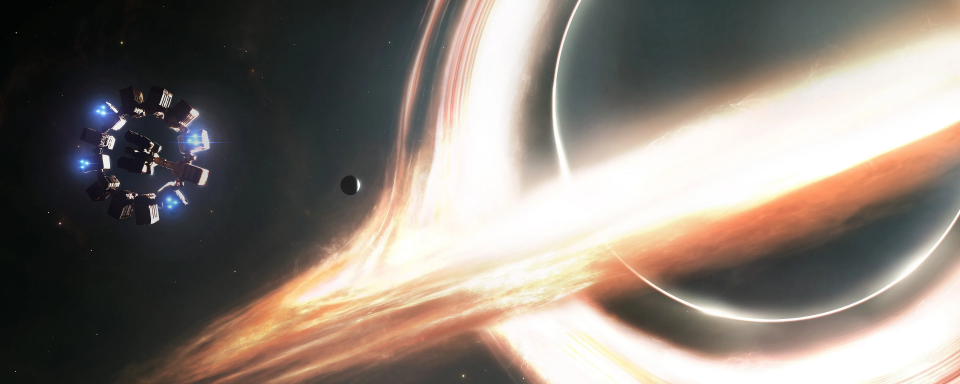
\includegraphics[width=\linewidth]{images/gargantua.png}
}

  Given that Gargantua's mass is $M=\qty{2.0e38}{kg}$, calculate the distance $r_{\text{e}}$ of Miller's planet from the black hole.
\end{enumerate}
\end{exercise}



\section{Space}
\label{sec:space}

\subsection{Distances}
\label{sec:distances}

Together with the notion of time, also the notions of space and distance lose some of their traditional intuition. Traditionally when we speak of the distance of a moving object at a given time, we mean the distance at the same instant of time, measured on a straight line. But we have seen that it does not make sense for us to ask \enquote{what is the time for the object, right now?}; and moreover, spacetime is curved. Owing to the path-dependence of time and to curvature, we can define and measure several \enquote*{distances}, which are \emph{not} equivalent to one another.

\medskip

%
\marginpar{\vspace{-\baselineskip}\centering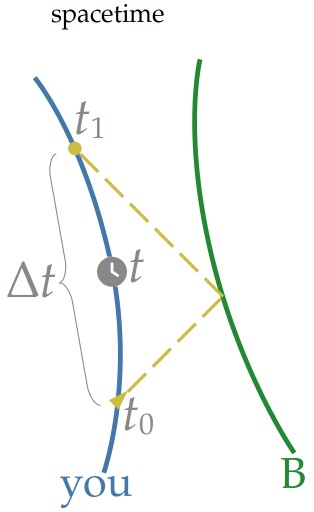
\includegraphics[width=0.9\linewidth]{images/radar_distance.jpg}%
  % \\[\jot]\footnotesize\flushleftright\color{mpcolor}%
}%
If an object~B is enough close to you, we define the \textbf{radar distance} of B from you at your particular proper time $t$ in the following way, illustrated in the side figure. The figure shows your \emph{worldline} in spacetime (similarly to what we did in \fig~\ref{fig:ABC_spacetime}) in \textcolor{blue}{blue} on the left, and the worldline of object~B in \textcolor{green}{green} on the right. At your proper time $\yti$ you send a light pulse towards object~B. The pulse travels in empty space, and upon hitting object~B it immediately bounces back to you. It reaches you at your proper time $\ytf$. The worldline of the light pulse is the \textcolor{yellow}{dashed yellow} line. A proper time $\Dt = \ytf - \yti$ has elapsed for you between emission and reception of the light pulse, and the time exactly in between emission and reception is $t = (\ytf + \yti)/2$. The radar distance $d$ of object~B from you at time $t$ is then defined as
\begin{equation}
  \label{eq:physical_distance}
  d \defd \tfrac12 c\, \Dt
\end{equation}
where $\yc$ is the speed of light in vacuum, a universal physical constant:
% %
% \marginpar{\vspace{-\baselineskip}%
%   \footnotesize\color{mpcolor}The SI symbol for the speed of light in vacuum is \enquote{$c_{0}$} \parencites[item~6-35.2]{iso2008}. For simplicity we shall omit the subscript \enquote{${}_{0}$} in these notes.%
% }%
\begin{equation}
  \label{eq:c}
  \yc = \qty{299792458}{m/s}\quad\text{(exactly).}
\end{equation}

%
\marginpar{\vspace{-\baselineskip}\centering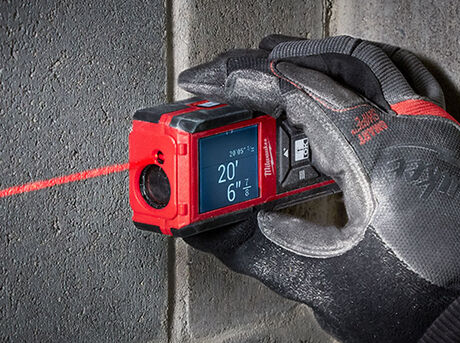
\includegraphics[width=0.75\linewidth]{images/laser_meter.jpg}%
\\[\jot]\footnotesize\flushleftright\color{mpcolor}A laser distance meter (the light beam is not visible in reality).%
}%
The \furl{https://www.nist.gov/si-redefinition/meter}{metre}, SI unit of length, is based on the measuring procedure above. Common laser distance meters also work by the same procedure, and therefore yield radar distance. When we speak of \enquote*{physical} distance, we typically mean radar distance.

Radar distance, however, makes sense only if the time lapse $\Dt$ is small enough, so that the relative motion between you and the object is approximately uniform. For this reason this distance cannot be used if the object is too far away: the farther away it is, the longer it takes for a light beam to travel to and fro. Radar distances can be used between the Earth and other Solar System planets; but they cannot be used for galaxies or other distant cosmological objects.

The value of the radar distance \emph{depends on the relative motion} between you and the object. Imagine that a friend of yours is located very close to you at time $t$, but is moving with respect to you. Upon measuring object~B's radar distance, your friend will generally find a value different from yours. The discrepancy between you and your friend's measured values will be the larger, the higher is the relative velocity between you two. Several observers in motion with respect to one another will generally disagree on the dimensions of an approximately rigid objects in their vicinity.


%
\marginpar{\vspace{-5\baselineskip}\centering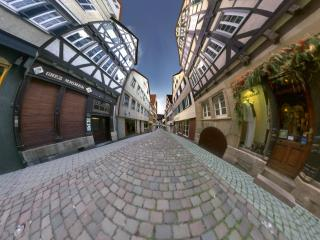
\includegraphics[width=\linewidth]{images/tuebingen.jpg}%
  \\[\jot]\footnotesize\flushleftright\color{mpcolor}How a street in T{\"u}bingen would look like (except for colour and some other features) if we travelled through it at around \qty{240000000}{m/s} (from \textit{\furl{https://www.spacetimetravel.org/}{Relativity visualized}})%
}%
The dependence on relative motion also affects, at high speeds, how we \emph{see} objects, which appears more and more deformed. You can find beautiful visualizations, both static and animated, at \textit{\furl{https://www.spacetimetravel.org/}{Relativity visualized}}.


\medskip

Given a coordinate time it is possible to define an alternative distance, which we can call \textbf{spatial coordinate distance} or just \enquote*{coordinate distance} for short. It is the length of the path joining you and the object at coordinate time $t$ for both; all points of the path are also understood to be at coordinate time $t$ as well. The path should be a \emph{straight line} between you and the object; but we must remember that spacetime is curved. The notion closest to a \enquote*{straight line} in a curved space is that of a \furl{https://mathworld.wolfram.com/Geodesic.html}{\emph{geodesic}}. It turns out that there may be several geodesics connecting you and the object at coordinate time $t$. This fact may lead to some complications. For instance there may be different paths having shortest distance; therefore saying \enquote{the path of shortest distance} may be ambiguous.

Coordinate distance has two advantages. First, it does \emph{not} depend on the relative motion between you and the object. Second, it can also be defined for very faraway objects. It is often difficult to measure directly, however, and often can only be extrapolated.

Note also that the speed of light defined with respect to coordinate distance need not have the value $\yc$ or even be constant! You might have heard or read about  distant cosmological objects, like \furl{https://esahubble.org/wordbank/quasar}{quasars}, that are said to be receding from us at speeds faster than light's. How is that possible? The reason is that the \enquote*{speeds} they're talking about are defined with respect to \emph{coordinate distance}, not radar distance.

\medskip

Many other distances -- and corresponding speeds -- can be defined; \furl{https://doi.org/10.48550/arXiv.astro-ph/9905116}{cosmology uses a plethora of them}. One must therefore be careful about which definition of distance is being used.

Luckily, for objects and events that are not too far away, and for observers whose relative speeds are not too high compared to the speed of light, all differently defined distances have very small discrepancies. In many everyday situations we can therefore speak of \enquote*{distance} without specify exactly which distance we're using. As an example, consider a car moving on a road at \qty{100}{km/h}, that is around \qty{28}{m/s}. The car's driver measures the length of the car to be \qty{4}{m} by radar distance. A pedestrian that sees the car passing by instead measures its length to be \qty{3.99999999999998}{m} by radar distance, which in this case is also equal to coordinate distance. This is a negligible measurement discrepancy in many ordinary situations.

The distances we'll use in these notes can be interpreted either as coordinate distances or as radar distances.

\medskip

% %
% \marginpar{\vspace{0\baselineskip}\centering%
% %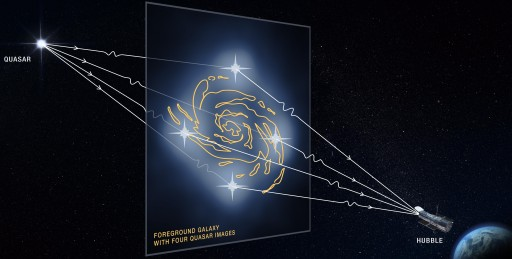
\includegraphics[width=\linewidth]{images/gravitational_lens3.jpg}%
% 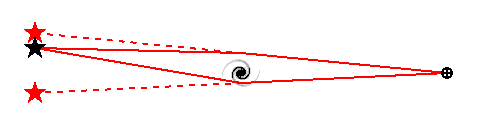
\includegraphics[width=\linewidth]{images/gravitational_lens1.png}%
% \\[2ex]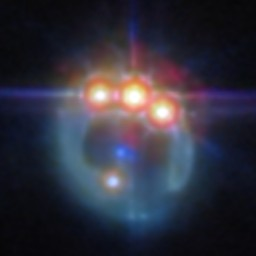
\includegraphics[width=\linewidth]{images/quasar_lens2.jpg}%
% \\[\jot]\footnotesize\flushleftright\color{mpcolor}Top: from
% %\furl{https://www.jpl.nasa.gov/images/pia23641-gravitational-lensing-graphic}{NASA JPL}.
% \emph{\furl{https://www.astro.ucla.edu/~wright/distance.htm}{The ABC's of Distances}}.
% Bottom: from \furl{https://esawebb.org/images/potm2406a}{ESA/Webb}.%
% }%
%
\marginpar{\vspace{0\baselineskip}\centering%
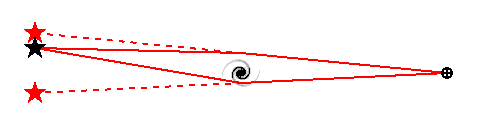
\includegraphics[width=\linewidth]{images/gravitational_lens1.png}%
\\[\jot]\footnotesize\flushleftright\color{mpcolor}From
\emph{\furl{https://www.astro.ucla.edu/~wright/distance.htm}{The ABC's of Distances}}.%
}%
\marginpar{\vspace{0\baselineskip}\centering%
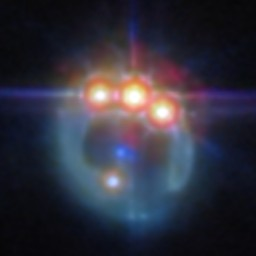
\includegraphics[width=\linewidth]{images/quasar_lens2.jpg}%
\\[\jot]\footnotesize\flushleftright\color{mpcolor}From \furl{https://esawebb.org/images/potm2406a}{ESA/Webb}.%
}%
A spectacular case of the effect of spacetime curvature is the phenomenon of \furl{https://science.nasa.gov/mission/hubble/science/science-behind-the-discoveries/hubble-gravitational-lenses}{gravitational lensing}. Owing to the curvature of spacetime, light and other electromagnetic radiation emanating from the object reach us along different paths in spacetime. All these paths are \enquote{straight lines} (geodesics). Coming from different directions, to us these look like distorted, duplicated images of the object, as schematized in the top side figure. The curvature is generated by some large distribution of energy-mass, such as a galaxy, between us and the object. A beautiful example of this phenomenon is given by the \furl{https://www.nasa.gov/image-article/distant-quasar-rx-j1131}{quasar RX~J1131-1231}, bottom side image. Spacetime curvature separates the light arriving to us from this quasar into four \textcolor{yellow}{yellow} \amp\ \textcolor{red}{red} spots, three at the top and one at the bottom in the image. The curvature is generated by a galaxy visible as the \textcolor{blue}{blue spot} at the centre.% but get also deformed into the almost-closed \textcolor{blue}{blue arc}.

\medskip

Length and distance have SI dimension \enquote*{\textsf{length}}, and we shall usually measure them using the unit \emph{metre}, symbol \enquote*{$\unit{m}$}.

\begin{exercise}[label={ex:distance}]
  % **** Add figure
  Imagine that you and a friend of yours are measuring your distance from a wall, using a laser distance meter each. You and the wall are static with respect to Earth's surface. Your friend is moving with a speed $v$ towards the wall, and is right beside you at the exact moment of the measurement.

  \smallskip

  In this specific situation, if $d_{\textrm{you}}$ is the distance measured by you, and $d_{\textrm{friend}}$ the distance measured by your friend, the two are related by the formula
  \begin{equation*}
    d_{\textrm{friend}} = d_{\textrm{you}} \cdot \sqrt{1 - v^{2}/\yc^{2}} \ ,
  \end{equation*}
  where $\yc$ is the speed of light, given in \eqn~\eqref{eq:c}. Note that this formula is also valid if your friend is moving away from the wall, rather than towards it.

\begin{enumerate}[exerc]
\item\label{item:distance_friend} Suppose you find that the distance of the wall from you is \qty{200}{m}. Your friend's speed is \qty{300}{m/s}. How much is the distance from the wall to your friend, who's right beside you, as measured by your friend? (You'll need a high-precision calculator and 18 significant digits.)

\item\label{item:velocity_friend} Now instead suppose you find that the distance of the wall from you is \qty{500}{m}. Your friend measured (when right beside you) a distance of \qty{499}{m}. How fast was your friend moving?
\end{enumerate}
\end{exercise}

\subsection{Spatial coordinates}
\label{sec:coord_space}

The peculiarities of space and the curvature of spacetime can make it difficult to communicate the positions of objects and events by relying on distances. In giving indications about the location of a shop we can say \enquote{it's 200 metres down the road} without ambiguity. But in situations where much higher precision is needed and extreme motions or gravitational fields are involved, we would need to know the velocity of the person we're talking to, because the distances measured by us and by that person could be very different. Moreover, the communication of locations usually involves reference to places that are known to all parties involved in the communication.

These problems are all bypassed by using a \textbf{spatial coordinate system}, or \enquote*{coordinate system} for short. A coordinate system is the assignment, by agreement, of three numerical labels to every point in a given region of space, \emph{for each coordinate time}. We use symbols for these labels, such as $(x,y,z)$ or $(r, \theta,\phi)$ or others. The values of these labels are thus the same for all observers. Often these labels have physical meaning, such as the distance from some event as measured by a specific observer, but they don't need to. In situations where only two or just one dimension are relevant, we can just use two or one spatial coordinates. Note that a coordinate system is usually defined on a limited region of space.

%
\marginpar{\vspace{-\baselineskip}\centering%
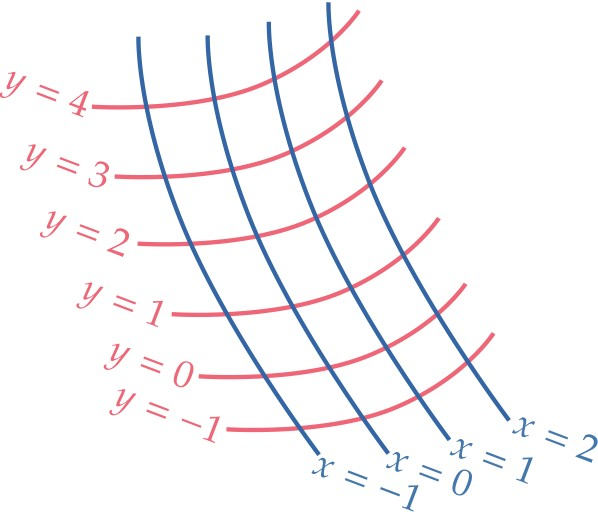
\includegraphics[width=\linewidth]{images/coords_curv.jpg}%
% \\[\jot]\footnotesize\flushleftright\color{mpcolor}%
% Grid representing a two-dimensional coordinate system.%
}%
A coordinate system can be visualized as a grid made by a set of lines or planes, one set for each coordinate, which allow us to read the coordinates of any point. The side figure shows an example with coordinates $(x,y)$ in two dimensions. It is of course assumed that the grid can be refined as much as needed. We are all familiar with the coordinate system $(\lambda, \phi)$ of \emph{latitude} and \emph{longitude} to identify locations on Earth's surface, and used internally by the location systems of mobile phones.

Whereas in the case of time we typically use a standard time coordinate~\autoref{sec:coord_time}, in the case of spatial coordinates we typically use more freedom: we set up peculiar coordinate systems adapted to the physics problem. In many exercises in these notes you'll see sketches of tailor-made reference systems.

\medskip

Spatial coordinate systems may be constructed so as to have particular physical properties, which in turn may lead to simpler expressions for some physical laws, \autoref{sec:constitutive}{as we shall see later}. For instance, the coordinate lines of a coordinate system might be straight lines (geodesics). If they are not, then we call the coordinate system \emph{curvilinear}; the coordinates in the previous side figure are an example.

One useful property for a coordinate system is to have its coordinate lines always \emph{orthogonal} to one another, that is, they intersect at $\pi/2\:\unit{rad}$ at every point. We call this an \textbf{orthogonal coordinate system}. In these notes we shall always use orthogonal coordinates. A coordinate system can be curvilinear \emph{and} orthogonal.

\begin{exercise}[label={ex:latlong}]
  % **** Add figure
 On Earth's surface we often use the system of two coordinates called \emph{latitude} and \emph{longitude}. Coordinate lines of constant latitude are called \emph{parallels}; those of constant longitude are called \emph{meridians}. Earth's surface is curved, and the \enquote{straight lines} in this space are maximal circles. All the meridians are maximal circles; therefore longitude is \emph{not} a curvilinear coordinate.

 \begin{enumerate}[exerc]
 \item\label{item:latitude_curvilinear} Is latitude a curvilinear coordinate? Explain why or why not.

 \item\label{item:latlong_ortho} Are latitude and longitude orthogonal coordinates? Explain why or why not.
\end{enumerate}
\end{exercise}





%
\marginpar{\vspace{\baselineskip}\centering%
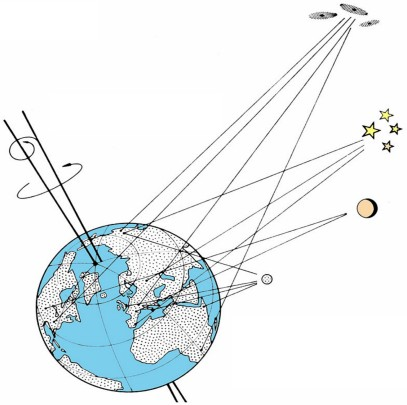
\includegraphics[width=\linewidth]{images/gcrf.jpg}
\\[\jot]\footnotesize\flushleftright\color{mpcolor}%
The assignment of coordinates on and around Earth depends on nominal values assigned to distant astronomical objects (from \cites{capitaine2010})%
}%
\mynotew{to be continued}





%%%% Time space end





:\enspace
\begin{enumerate*}[label=(\arabic*)]
\item how many people are in the rear half, right now;\enspace
\item how many people are crossing the imaginary division between the front and rear half during one minute, starting from now.
\end{enumerate*}



The more an observer's speed is close to the speed of light in vacuum $\yc$, a universal physical constant:
%
\marginpar{\vspace{-\baselineskip}%
  \footnotesize\color{mpcolor}The SI symbol for the speed of light in vacuum is \enquote{$c_{0}$} \parencites[item~6-35.2]{iso2008}. For simplicity we shall omit the subscript \enquote{${}_{0}$} in these notes.%
}%
\begin{equation}
  \label{eq:c}
  \yc = \qty{299792458}{m/s}\quad\text{(exactly).}
\end{equation}







Let's say that we want to measure the \enquote*{distance} of a moving object; a couple of problems appear. One problem is that when we speak of the distance of an object, traditionally we mean the distance between us and the object \enquote{at the same instant of time}. But as we have seen, it does not make sense for us to ask \enquote{what is the time for the object, right now?}. We could bypass this problem by specifying \enquote{when our clock shows time $a$ and the object's clock shows time $b$}, instead of saying \enquote{now}. Another problem appears, though. Distance is traditionally measured along a \emph{straight line} between us and the object. But spacetime is curved. The closest notion to a \enquote{straight line} is that of a \furl{https://mathworld.wolfram.com/Geodesic.html}{\emph{geodesic}}. It turns out, however, that there may be several geodesics connecting us at our time $a$ and the object at its time $b$, and the distances measured along these geodesics will generally be different. The very notion of \enquote*{distance} therefore becomes tricky and has different and non-equivalent definitions.








Luckily, for objects and events that are not too far away, and for observers whose relative speeds are not too high compared to the speed of light, all differently defined distances have very small discrepancies. In many everyday situations we can therefore speak of just one unique distance, up to some precision. As an example, consider a car moving on a road at \qty{100}{km/h}, that is around \qty{28}{m/s}. The car's driver measures the length of the car to be \qty{4}{m}. A pedestrian that sees the car passing by instead measures its length to be \qty{3.99999999999998}{m}. This is a negligible measurement discrepancy in many ordinary situations.
%
\marginpar{\vspace{-8\baselineskip}\centering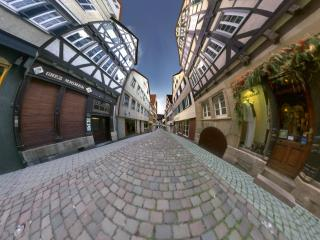
\includegraphics[width=\linewidth]{images/tuebingen.jpg}%
  \\[\jot]\footnotesize\flushleftright\color{mpcolor}How a street in T{\"u}bingen would look like (except for colour and some other features) if we travelled through it at around \qty{240000000}{m/s} (from \textit{\furl{https://www.spacetimetravel.org/}{Relativity visualized}})%
}%
These peculiarities of space and time also affect, at high speeds, how we \emph{see} objects. You can find beautiful visualizations, both static and animated, at \textit{\furl{https://www.spacetimetravel.org/}{Relativity visualized}}.



\smallskip

The discrepancies between distances measured by different observers, and the fact that in some cases there is no uniquely defined distance, lead to difficulties in the locating events. As in the case of time we can bypass these difficulties by agreeing on a set of three unique numbers assigned to each event at each coordinate time, called the \emph{spatial coordinates} of that event. We discuss them in the next section. When we use spatial coordinates, some important physics formulae turn out to be the same no matter whether we use General Relativity or an approximate theory such as Newtonian Mechanics.






\iffalse
\newpage
\nonoaddchap{Introduction}
\label{sec:intro}

% %\setlength{\beforeepigraphskip}{0pt}
% %\setlength{\afterepigraphskip}{0pt}
\epigraph{The loss implied in such an acquisition can be estimated only by those who have been compelled to unlearn a science that they might at length begin to learn it.}{J. C. Maxwell \cites*{maxwell1878}}



Until some decades ago, the 18th-century physical notions typically taught in introductory Bachelor physics courses were enough to prepare an engineer for future specializations and jobs. Students who wanted to venture into modern theories, such as Relativity, were required to \textbf{re-learn} some of the most important physical notions -- \emph{Energy}, mass, time, entropy above all -- which in these theories are quite different from the 18th-century ones. But at that time the modern theories  still mostly had only theoretical, not practical, importance. So the re-learning efforts of the curious students could perhaps be justified.

%% \mynotew{add about re-learning necessary for continuum mechanics}

\smallskip


% \marginpar{\footnotesize%
% {\color{mpcolor}\enquote{\emph{The achieved performances of atomic clocks and time
% transfer techniques imply that the definition of time scales
% and the clock comparison procedures must be considered
% within the framework of General Relativity}}\sourceatright{\cites{petitetal2005}}}
% }
\marginpar{%
\color{mpcolor}\footnotesize%
    \enquote{\emph{Numerous relativistic issues and effects play roles in the global positioning system, on which millions of drivers, hikers, sailors, and pilots depend to find out where they are. The GPS system is, in effect, a realization of Einstein's view of space and time. Indeed, the system cannot function properly without taking account of fundamental relativistic principles.}}\sourceatright{\cites{ashby2002}}
}
%
That situation has changed today. Modern theories and modern physical notions are an essential part of many everyday technologies, like nuclear reactors and the \furl{https://www.gps.gov}{Global Positioning System} (see the entertaining discussion in \cites[Project~A]{tayloretal2000}, and also \cites{petitetal2005,fliegeletal1996,ashby2002,muelleretal2008}). Modern theories and modern physical notions are required for the development of new technological possibilities, from \furl{https://www.ibm.com/topics/quantum-computing}{quantum computers} to solar sails, such as NASA's \furl{https://www.nasa.gov/mission/acs3/}{Advanced Composite Solar Sail System}. An engineering student (including communication, computer, and data engineering) may likely end up in a job that requires an understanding of modern physical notions. The diffusion of \furl{https://www.ibm.com/topics/large-language-models}{large language models} will moreover lead to a future demand for engineers who actually \textbf{understand} those physical notions, not little monkeys who have been trained to mechanically manipulate some equations while throwing some technobabble around. Automated large language models are faster, cheaper, and more precise in doing this kind of monkey activities. So why should one hire a human to do the same?

While moving from the older to the newer notions often requires re-learning efforts and conceptual re-orientations, the move in the opposite direction is less demanding. The modern physical notions are more encompassing than their 18th-century parents. Their understanding leads to an understanding of their older counterparts as approximate and special cases. Students, moreover, have often been hearing quite early  about the new notions from mass media; for instance about the equivalence of mass and energy, or about the discrepancy in time reckoning by different observers. Owing to this early exposure, students sometimes ask very intelligent and deep questions -- for instance \enquote{\emph{should the mass of the body be included in its internal energy?}} -- when exposed to the old notions.



\medskip

It is therefore high time that introductory Bachelor physics courses be based on modern physical notions. Students should not be required to waste time and mental effort to learn something that they must unlearn and re-learn, only because of the inertia of academia and teachers.

Some teachers say \enquote{it would be too difficult for students to understand modern ideas, because they are too familiar with the old ones. This is why we need to teach the old and slightly incorrect ideas first, and correct them later}. I think that this kind of reasoning is scientifically unacceptable and leads to a vicious circle. Students are unfamiliar with new notions only because they were raised by a generation who was taught old ones. New notions become familiar only after a couple of generations learn them at an early stage. This is obvious if you consider that notions like \enquote{energy}, \enquote{electromagnetic field}, \enquote{vector} are very familiar today, but were absolutely \emph{un}familiar a century or so ago. If we had always taught what's familiar, then we would still be teaching about the \emph{air, earth, water, fire} elements, and that the Sun revolves around the Earth. Arguments in favour of teaching old notions are for the most part just pretexts for laziness.

\medskip

The present lecture notes are an experiment and attempt to introduce classical mechanics and thermodynamics from modern physical notions and viewpoints. The core equations remain the same, but the students should have a broader conception of their meaning and of the symbols that appear in them.

\iffalse % replies from NASA/JPL, 2024-04-12
  "Yes, NASA/JPL include relativistic effects when we plan or calculate trajectories for Earth, Moon, and beyond.  The same PPN (parameterized post-Newtonian) metric is used to calculate and plan spacecraft dynamics.  For example, if we don’t include the relativistic effect, GPS orbits will be not as good as what we have now. 😊" Ryan Park, Group Supervisor of JPL's Solar System Dynamics Group

   "Further to what Ryan said, we use the same dynamical models for navigating in cis-lunar or geocentric space as we do for interplanetary missions: the physics doesn’t change between the two regimes, and the same software is use for navigating in both regimes.

It seems the professor has already found the key document by Moyer, which I would have referenced myself. In fact, I used the relativistic expressions in Moyer’s earlier internal JPL document when I coded up the dynamical models used in our Small Body software, back in the early ‘90s, and the same Moyer expressions were used in JPL navigation software for a couple decades before that (back at least to the ‘70s)." Paul Chodas, JPL's director for the Center of Near Earth Object Studies.
\fi


% ** 6
% *** Importance of physics, necessity of maths: numbers (precision) and formulae (compact relations)
% *** Different languages (show examples) and points of view. What's chosen here
% *** Arena for physics (one point of view): space, time, "stuff"
%

\printpagenotes*
\fi


%% old parts of the book
\iffalse
\printpagenotes*
\clearpage
\nonochapter{Conservation of matter}
\label{ncha:cons_matter}

\epigraph{\emph{%
\enquote{What you do in this world is a matter of no consequence,} returned my companion, bitterly. \enquote{The question is, what can you make people believe that you have done?\textellipsis}%
}}{Sherlock Holmes (A. C. Doyle) \cites*{doyle1887}}

\nonosection{Formulation and generalities}
\label{nsec:cons_matter_formulation}

Choose an arbitrary sequence of closed control surfaces between coordinate times $\yti$ and $\ytf$, enclosing a sequence of control volumes. Denote by $\yN(t)$ and $\yJ(t)$ the amount of matter in the control volume and the influx through the control surface at time $t$. Then the law of \textbf{conservation of matter} is expressed by either of the equations
\begin{definition}{Conservation of matter}
  \begin{equation}
    \label{neq:cons_matter}
    \begin{gathered}
      \underbracket[0pt]{\yN(\ytf) - \yN(\yti) - \int_{\yti}^{\ytf}\!\!\yJ(t)\,\di t = 0}_{\mathclap{\text{\color{grey}integral form}}}
      \qquad%\text{\footnotesize\color{grey}or}
      \qquad
      \underbracket[0pt]{\frac{\di\yN(t)}{\di t} - \yJ(t) = 0}_{\mathclap{\text{\color{grey}differential form}}}
    \end{gathered}
  \end{equation}
\end{definition}

Conservation of matter is a law that we intuitively take for granted and use continuously in our life. The very notion of \enquote*{object} -- including living objects -- is possible thanks to this fundamental regularity of nature: we can speak of objects because they exist for some time and we can follow them as they move in space. % This is possible because the integrated flux through a small surface of the \enquote{stuff} that makes the object equals the amount that disappeared in a nearby small region: we can then say that the \enquote{stuff} has moved.

% In fact even the notion of \emph{velocity} of an object is actually built from the notions of flux and of volume content, but it would make little sense if the flux didn't equal the rate of change of the volume content.
% \begin{extra}{Velocity from flux and volume content}\label{nextra:velocity_matter}
%   Suppose we have a coordinate system $(t,x,y,z)$. Consider a small spatial region of cuboid shape delimited by two surfaces having $x$ constant, two having $y$ constant, and two having $z$ constant. The instantaneous velocity component $v_{x}$ is defined as the ratio of:
%   \begin{enumerate*}[label=(\alph*)]
%   \item the flux $\yJ_{x}$ through any of the two $x$-constant surfaces, crossing in the positive-$x$ orientation, divided by surface area $A$, and
%   \item the volume content $\yN$ in the cuboid region, divided by the region's volume $V$:
%   \end{enumerate*}
%   \begin{equation*}
%     v_{x} \defd \frac{\yJ_{x}/A}{\yN/V}
%   \end{equation*}
%   And analogously for the other two velocity components. This relation is valid as a first approximation for enough small velocities and weak gravitational fields (Newtonian approximation).
% \end{extra}

\nonosubsection{Balances of matter}
\label{nsec:matter_balances}

The law of \emph{conservation} of matter holds, as far as we know, for all kinds of matter \emph{considered together}. \marginpar{\vspace{-\baselineskip}\footnotesize\flushleftright\color{mpcolor}%
    \emph{\enquote{All these operators conserve $B-L$, so in any superunified theory we expect $B-L$ to be conserved\textellipsis}}}%
  \sourceatright{\cites{wilczeketal1979}%
}%
More specifically, it seems to hold in extreme physical conditions if we count baryonic and anti-leptonic matter as \enquote*{positive} and leptonic and anti-baryonic matter as negative.

When we consider different kinds of matter, such as different chemical elements, individual conservation laws still hold and can be applied in many common and important physical situations.

For some kinds of matter, conservation does not hold, however; for example in the previously mentioned {phenomena involving radioactive decay and nuclear energy}. For these kinds of matter we can still apply a \emph{balance} law, with a non-zero supply or sink.


\nonosection{Examples of constitutive relations}
\label{nsec:matter_constitutive}

\nonosubsection{Relation between matter and \masse}
\label{nsec:const_matter_mass}

The most common constitutive relation used  together with conservation of matter is the one relating a constant amount of \masse\ $\yM$ to a particular amount of matter $\yN$:
\begin{definition}{Molar mass}
  \begin{equation}
    \label{neq:molar_mass}
    \yM = \yrho\, \yN
  \end{equation}
  where the proportionality constant $\yrho=\yM/\yN$ is called \textbf{molar-mass constant}, and depends on the kind of matter considered.
\end{definition}

For instance, in many physical phenomena involving water we assume the constitutive relation above, with a
of \furl{https://webbook.nist.gov/cgi/inchi/InChI\%3D1S/H2O/h1H2}{water molar-mass constant} of approximately $\yrho_{\mathrm{H_2O}}=\qty{0.0180}{kg/mol}$. If a volume contains $\yN=\qty{20}{mol}$ of water, we usually attribute to it a \masse\ of
\begin{equation*}
  \begin{split}
    \yM &= \yrho_{\mathrm{H_2O}}\, \yN
    \\
    &=\qty{0.0180}{kg/mol} \times \qty{20}{mol}
    \\
    &= \qty{0.36}{kg}\,.
  \end{split}
\end{equation*}

The exact value of the molar-mass constant depends not only on the substance but also on the context and application: the substance may actually consist of a mixture of different kinds of matter. \enquote*{Air} for example is a mixture of different chemical elements, and their proportion in the mixture may depend on physical conditions such as temperature, and on geographical position.
\marginpar{\vspace{0\baselineskip}\centering%
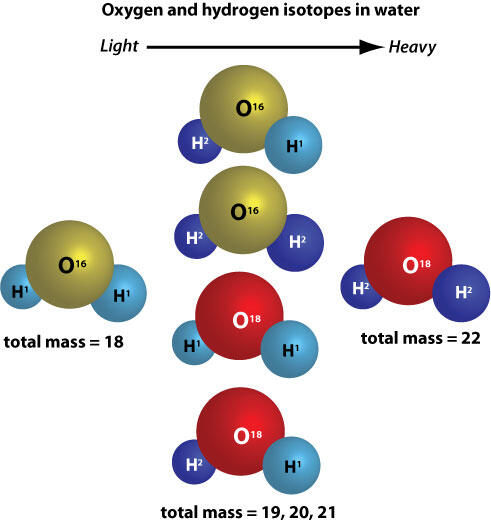
\includegraphics[width=\linewidth]{images/water_isotopes.jpg}%
\\[\jot]\footnotesize\flushleftright\color{mpcolor}%
There are several different isotopes of water, with different masses (image from \furl{https://www.usgs.gov/media/images/water-isotopes-diagram}{U.S. Geological Survey})%
}%
\enquote*{Water} is a mixture of different \furl{https://www.britannica.com/science/isotope}{isotopes} (molecules differing in the number of neutrons), and again the mixture proportions may vary with physical conditions.

The constant relating \masse\ and amount of matter is the same for volume contents and for fluxes. So to a matter flux $\yJ$ we can associate a \masse\ flux $\yrho\yJ$. For instance, if through a surface there's a flux of $\yJ=\qty{30}{mol/s}$ of water, then we associate to it a mass flux of
$$\yrho_{\mathrm{H_2O}}\,\yJ = \qty{0.0180}{kg/mol} \times \qty{30}{mol/s} = \qty{0.54}{kg/s}\,.$$

\smallskip

Using this constitutive relation we can re-express the conservation of matter in terms of mass. Suppose that for a given kind of matter the proportionality constant is $\yrho$; then conservation of matter implies
\begin{equation*}
  \begin{gathered}
    \yrho\yN(\ytf) - \yrho\yN(\yti) - \int_{\yti}^{\ytf}\!\!\yrho\yJ(t)\,\di t = 0
    \qquad%\text{\footnotesize\color{grey}or}
    \qquad
    \frac{\di\yrho\yN(t)}{\di t} - \yrho\yJ(t) = 0
  \end{gathered}
\end{equation*}
This is the \enquote*{law of conservation of mass}. Keep in mind that this is not a universal law: it's only an approximate law, only valid as long as the constitutive relation between matter and \masse\ is acceptable.

Phenomena for which this constitutive equation is no longer valid appear for example in particle physics, nuclear physics, and astrophysics.

\begin{exercise}
  At a particular time, a party balloon contains \qty{0.012}{kg} of Helium. A minute later, the same balloon contains \qty{0.010}{kg} of helium. Assume conservation of Helium, as well as a constitutive relation between amount and mass with \furl{https://webbook.nist.gov/cgi/inchi/InChI\%3D1S/He}{Helium molar-mass constant} $\yrho_{\mathrm{He}} = \qty{4e-3}{kg/mol}$.
  \begin{enumerate}[exerc]
  \item How much is the \emph{integrated efflux} of Helium, \textbf{in moles}, through the balloon's surface during the one-minute lapse of time?
  \item Assume that the efflux of Helium was constant in time during the one-minute time lapse. How much was the efflux of Helium, in moles/second?
  \end{enumerate}
\end{exercise}
\marginpar{\vspace{-11\baselineskip}\centering%

\includegraphics[height=7em]{images/helium_balloons.jpg}%
}



\nonosubsection{Relation between matter and momentum}
\label{nsec:const_matter_momentum}

Closely related to the previous constitutive relation is the one {relating an amount of matter and an amount of momentum}, briefly discussed before. Let us examine this constitutive relation more thoroughly.

Fix a coordinate system $(t,x,y,z)$. At a given point in space, take a small rectangular control surface of area $A$, with sides parallel to the coordinate axes $y$ and $z$. See side picture below. The surface must \emph{not} be moving in that coordinate system. Through this surface, in the positive-$x$ direction, there's a flux of matter that we denote $J_{x}$.

Construct two more surfaces of area $A$ through the same point in a analogous way: one parallel to the $zx$ axes and one to the $xy$ axes. The matter fluxes through them are $J_{y}$ and $J_{z}$.

Finally take a control volume of cuboid shape that fits the three surfaces. This cuboid has volume $V$, and contains an amount of matter $\yN$ and an amount of momentum $\yP$. Recall the {association between the matter flux} through the first surface and the velocity component $v_{x} \equiv \frac{J_{x}/A}{\yN/V}$, and similarly for the other two surfaces.

% Take a small control volume of cuboid shape, with side surfaces \emph{not moving} in the coordinate system $(t,x,y,z)$, and parallel to the $yz$-, $zx$-, and $xy$-coordinates. The cuboid has volume $V$ and each side surface has area $A$.
%
%   The control volume contains an amount of matter $\yN$. The flux across the side parallel to $yz$, in the positive-$x$ direction, is $\yJ_{x}$; and similarly for the other two directions. Remember from \sect\,\ref{nsec:fluxes_velocities} that we can consider the matter in the control volume as moving with velocity
%   \begin{equation*}
%     \yv = (v_{x}, v_{y}, v_{z}) = \frac{V}{A\,\yN}\, (\yJ_{x}, \yJ_{y}, \yJ_{z})
%   \end{equation*}
%
%   Then this control volume also contains an amount of momentum
% \marginpar{%
%     \footnotesize\flushleftright{\color{mpcolor}%
%       This is the famous relation that old textbooks take as the \emph{definition} of momentum.}}%
% \begin{equation*}
%   \yP = \yM\yv \equiv \yrho\,\yN\,\yv \equiv \yrho\, \frac{V}{A}\,
%   \begin{bmatrix}
%     J_{x}\\J_{y}\\J_{z}
%   \end{bmatrix}
% \end{equation*}
% The relation \enquote{$\yP=\yM\yv$} is the traditional one; but we see that it is completely equivalent to a relation between momentum and \emph{flux} of matter.

Assume that the constitutive relation between matter and mass, previously discussed, is valid, and associates a \masse\ $\yM=\yrho\yN$ to the amount of matter $\yN$.

\marginpar{\vspace{\baselineskip}\centering%
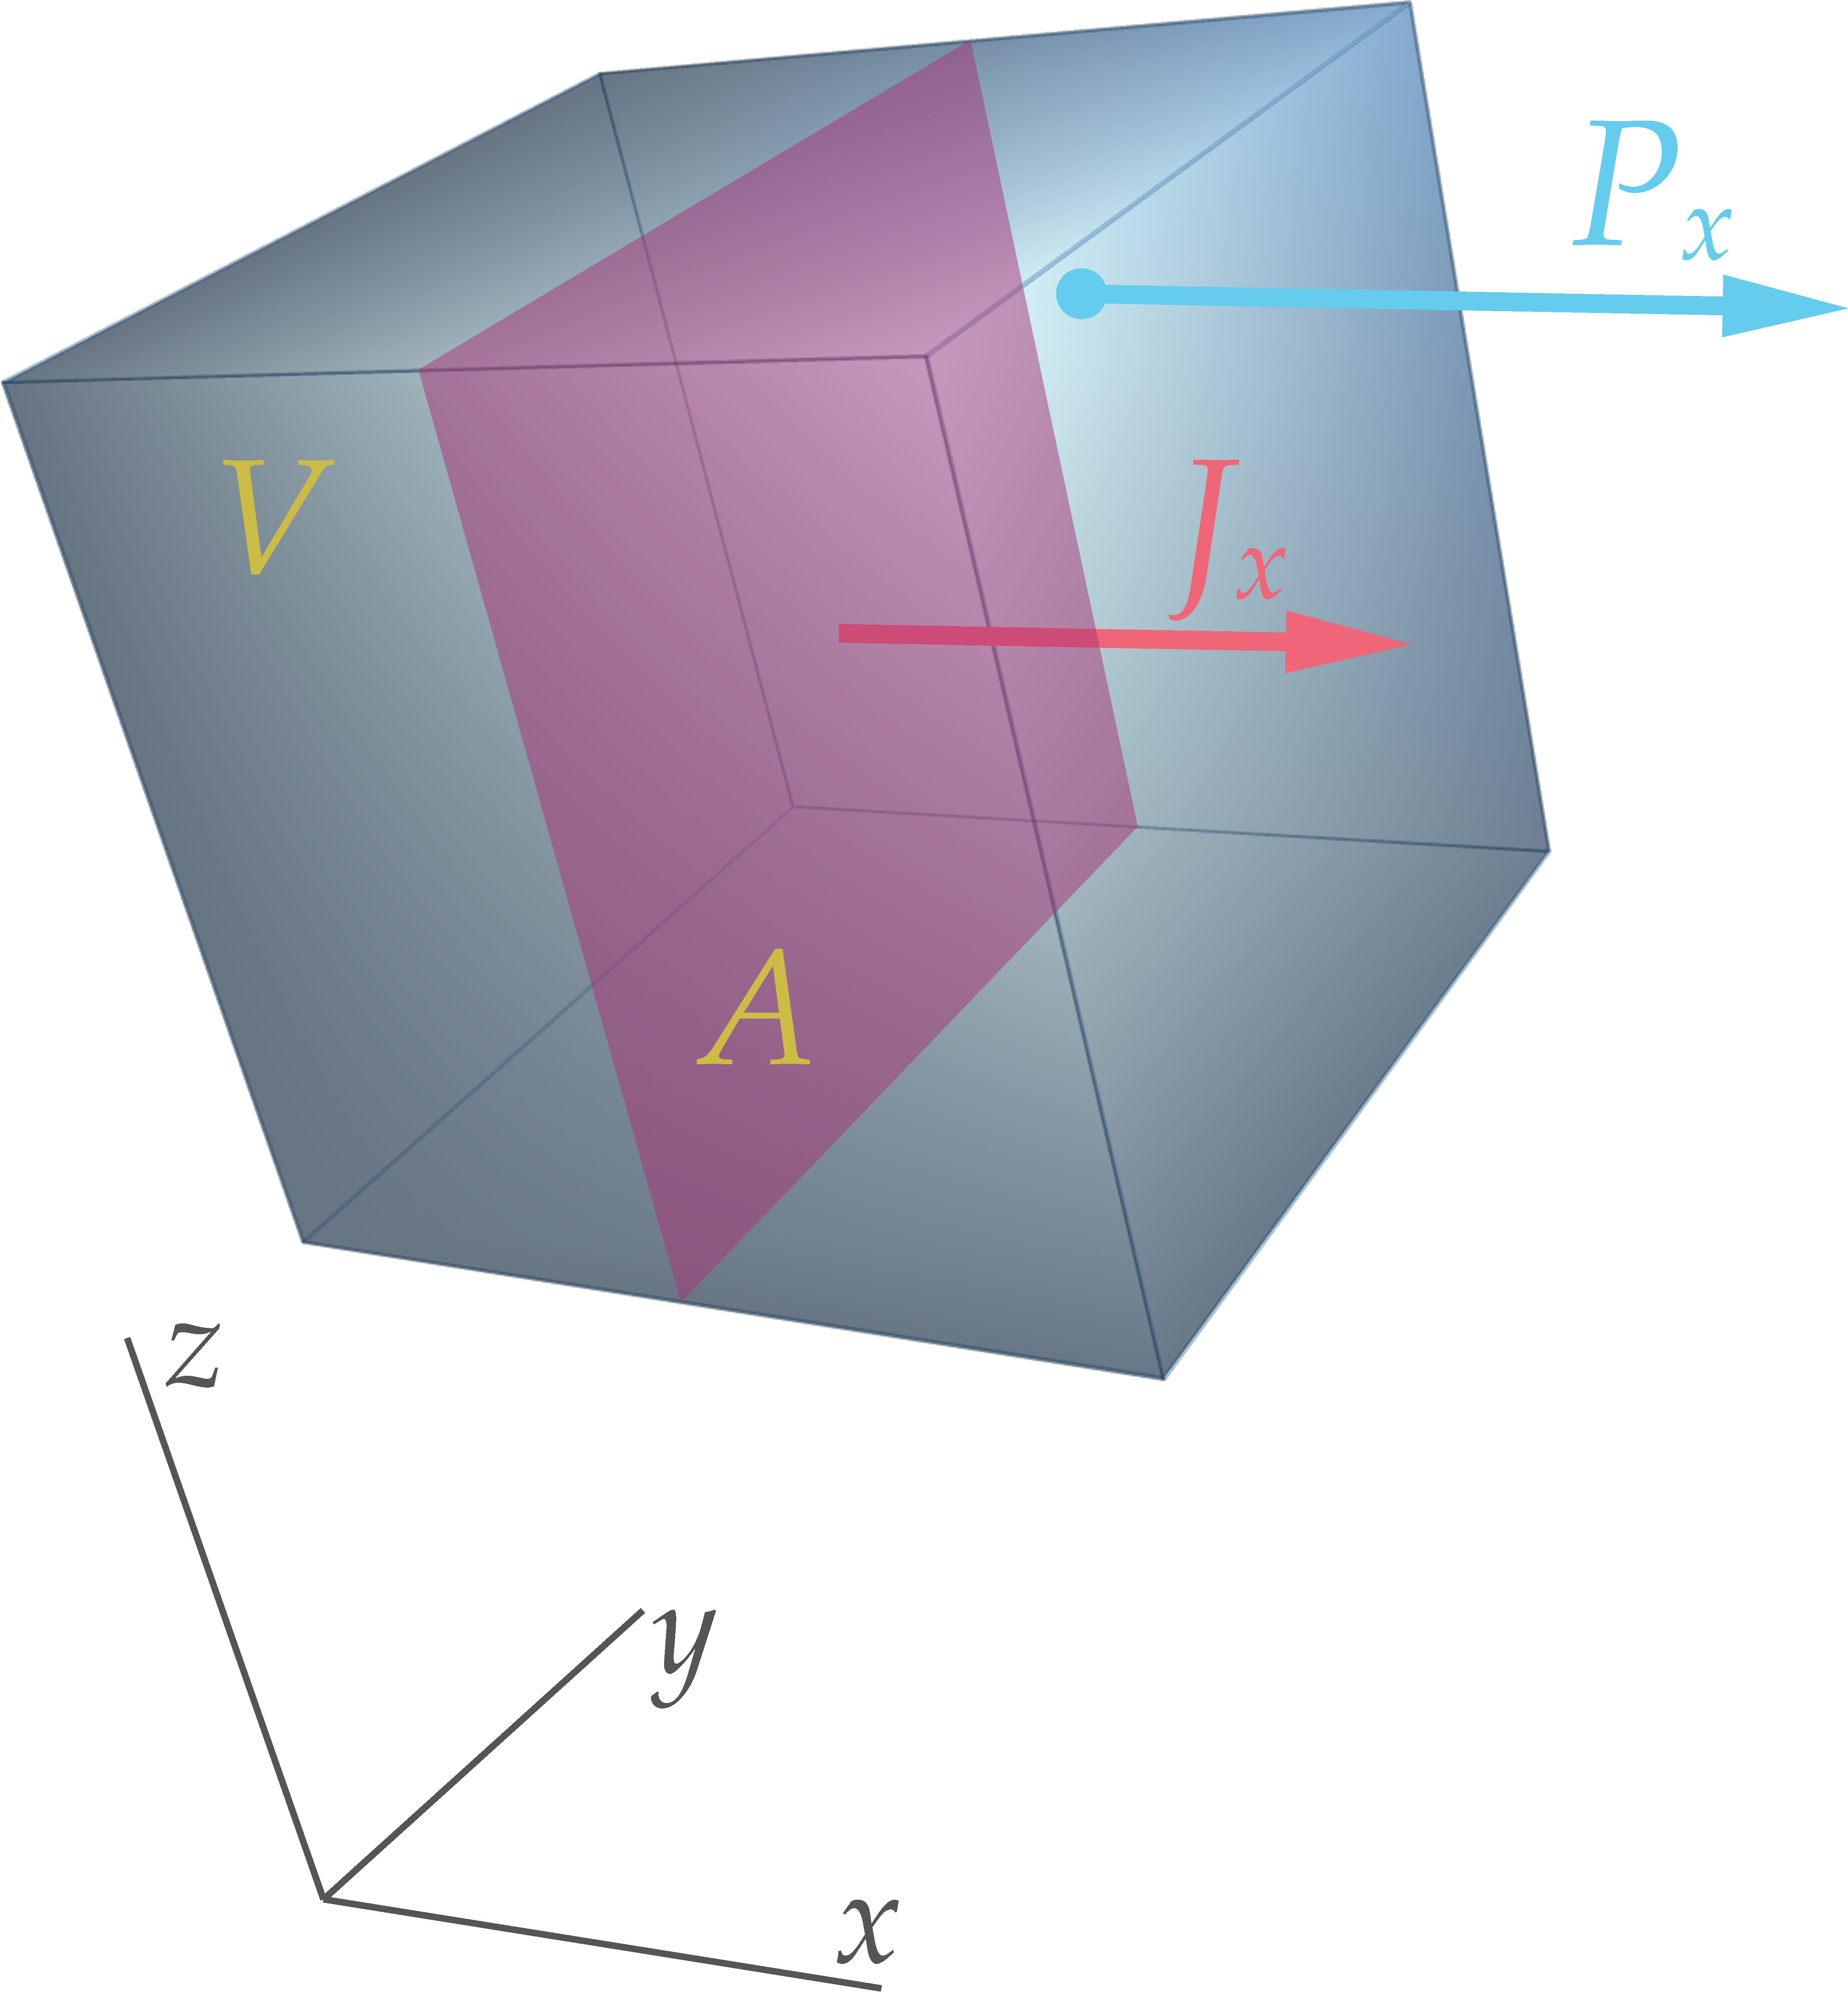
\includegraphics[width=\linewidth]{images/Px_Jx2.pdf}%
% \\[\jot]\footnotesize\flushleftright{\color{mpcolor}%
% }%
}%
\begin{definition}{Newtonian constitutive relation for momentum}
The \textbf{Newtonian relation for the momentum of matter} is a constitutive relation saying that the flux and velocity of matter and the volume content of momentum are proportional:
  \begin{equation}
    \label{neq:matter_momentum_Newton}
    \yP = \yM\yv = \yrho\, \frac{V}{A}\,
  \begin{bmatrix}
    J_{x}\\J_{y}\\J_{z}
  \end{bmatrix}
    % \qquad\text{with}\qquad
    % \yM=\yrho\yN
  \end{equation}
\end{definition}
This relation is only valid for very small areas and volumes (we should really take a limit), so small that the flux of matter or the volume content of momentum wouldn't change if we choose a surface and a volume in slightly different positions.

\bigskip

An analogous constitutive relation also exists between \emph{flux} of momentum and flux and volume content of matter. Its most general formulation involves many mathematical terms, so let's consider a simplified situation instead.
\begin{definition}{Convective flux of momentum (special case)}
Through the $yz$-surface above there's a flux of momentum
  \begin{equation}
    \label{neq:matterflux_force_Newton}
    \yF_{\text{conv}} = \yrho J_{x}\,\yv \equiv
    \yrho\, \frac{V}{A}\,\frac{J_{x}}{\yN}\,
  \begin{bmatrix}
    J_{x}\\J_{y}\\J_{z}
  \end{bmatrix}
    % \qquad\text{\color{midgrey}(also equivalent to\enspace$\yF=\yM\yv\,\yJ_{x}/\yN$)}
  \end{equation}
  called a \textbf{convective flux}. Analogous relations hold for the surfaces parallel to the $zx$ and $xy$ coordinates.
\end{definition}
\begin{warning}
  Usually there are additional, non-convective flows of momentum (forces) associated with matter, as we shall see later.
\end{warning}

These constitutive relations are only approximate and become incorrect when the speeds involved are close to the speed of light or the energy concentrations are so high to create strong gravitational fields (high spacetime curvature), or when some kind of electromagnetic phenomena are also involved.

In particular, according to the Newtonian constitutive relation, \emph{momentum and velocity of matter are always parallel}, because they are two vectors that differ by a multiplicative scalar. In general this is not exactly true: momentum can have a different direction from velocity. In General Relativity one must often take this fact into account.

\begin{extra}{More symmetric relation between mass \amp\ momentum and matter}
  When we work with \emph{densities}, which express the amounts of a quantity per unit volume or per unit surface, the relation between \masse\ \amp\ momentum on one side, and matter \amp\ its flux on the other, becomes more explicit and symmetric. We have
  \begin{equation*}
    \ym = \rho\yn \qquad \yp = \rho\yj
  \end{equation*}
  where $\ym$ and $\yp$ are the mass and momentum densities, and $\yn$ and $\yj$ are the matter and matter-flux densities.
\end{extra}


\smallskip

\begin{exercise}
  The side picture illustrates the section of a river. The river has an approximately \emph{steady flow} of water; this means that if we choose a static control volume anywhere in the river, such as the one in the depicted section, the amount of water $\yN$ therein is \emph{constant in time}.

  Assume that
  \begin{enumerate*}[label=(\alph*)]
  \item water satisfies conservation of matter;
  \item the amount of water in the illustrated volume is $\yN=\qty{4e5}{mol}$;
  \item water only flows across the imaginary vertical surfaces that delimit the river section on the front and back of the picture, cutting across the river.
  \end{enumerate*}
  \begin{enumerate}[exerc]
  \item What can you say about the two fluxes across the two imaginary vertical surfaces, each considered as crossed from right to left in the picture? Can you find their numerical values?

  \item You are told that the illustrated volume of water has total momentum $P=\qty{21600}{N\,s}$, directed from left to right perpendicularly to the imaginary vertical surfaces. Assuming the Newtonian constitutive relation for momentum, and the molar-mass constant $\yrho_{\mathrm{H_2O}}=\qty{0.0180}{kg/mol}$, can you find the values of the fluxes from the previous question?
  \end{enumerate}
\end{exercise}
\marginpar{\vspace{-19\baselineskip}\centering%
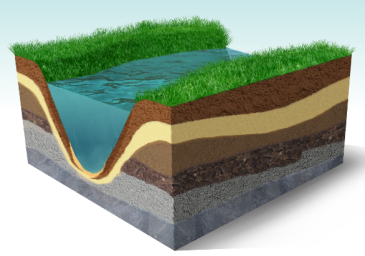
\includegraphics[width=\linewidth]{images/riverbed3.png}%
\\[\jot]\footnotesize\flushleftright\color{mpcolor}%
(Illustration by \furl{https://dribbble.com/squarefountain}{Cathryn Briggs})%
}%

\nonosubsection{Gas pressure}
\label{nsec:matter_const_thermodynamics}

In the previous section we saw a constitutive relation between matter and \emph{flux} of momentum, which we called \enquote*{convective flux}. It is a flux that's always present whenever there's matter in motion.

In some circumstances, matter gives rise to a flux of momentum even when it is not in (visible) motion. In such cases it is said to be in a \furl{https://www.britannica.com/science/gas-state-of-matter}{\emph{gaseous} state}. The most cogent example is the air around us, which has a continuous flux of momentum, of approximately \qty[print-unity-mantissa=false]{1e5}{N} on every square-metre of surface, called \furl{https://www.britannica.com/science/atmospheric-pressure}{\emph{atmospheric pressure}}. This flux is always {\emph{compressive}} and occurs through any surface: any imaginary surface within the body of air itself, and any real surface between air and any other object.

\smallskip

For some kinds of matter in a gaseous state, the magnitude of their compressive flux of momentum $\yF_{\text{press}}$ can be approximated by the formula:
% \marginpar{\vspace{3\baselineskip}\centering%
% 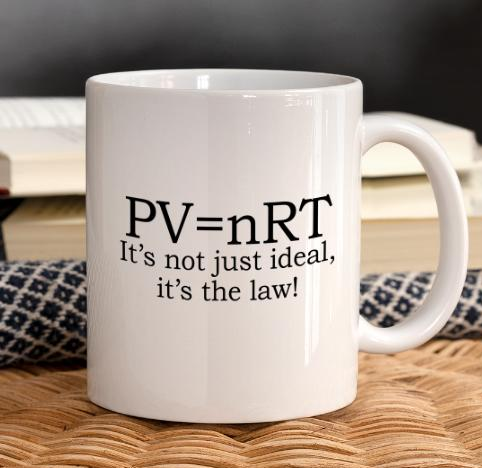
\includegraphics[width=\linewidth]{images/idealgas_mug.jpg}%
% % \\[\jot]\footnotesize\flushleftright{\color{mpcolor}%
% % The famous \enquote{$pV=NRT$} formula}%
% }%
\begin{definition}{Ideal-gas law}
  \begin{equation*}
    \frac{F_{\text{press}}}{A} = R\,\yT\,\frac{\yN}{V}
  \end{equation*}
  called the \textbf{ideal-gas law}, where $A$ is the area through which the momentum flux occurs, $V$ is the volume of a small region adjacent to the area, $\yN$ is the amount of matter in that volume, $\yT$ is its temperature, and $$R = \qty{8.31446261815324}{N\,m/(K\,mol)}\qquad\text{(exactly)}$$ is the \furl{https://www.britannica.com/science/universal-gas-constant}{molar gas constant}. The ratio $\yF_{\text{press}}/A$ of force and area is called \emph{pressure}.
\end{definition}
\marginpar{\vspace{-13\baselineskip}\centering%
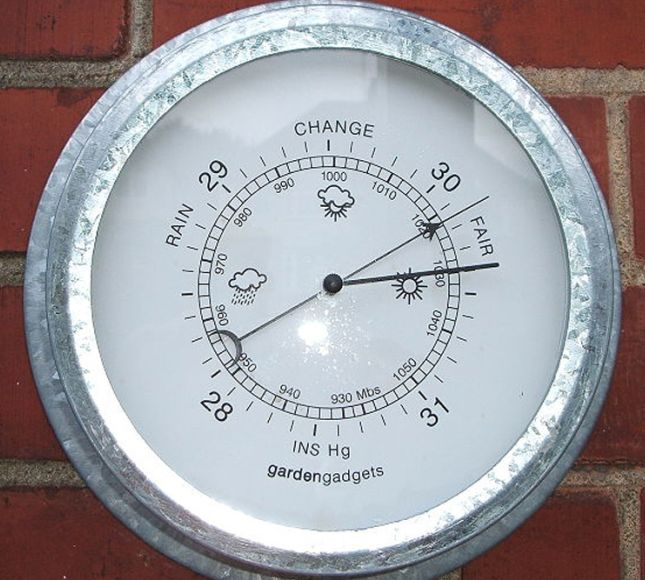
\includegraphics[width=\linewidth]{images/barometer.jpg}%
\\[\jot]\footnotesize\flushleftright\color{mpcolor}%
  A barometer for measuring atmospheric pressure (image from \furl{https://education.nationalgeographic.org/resource/atmospheric-pressure/}{National Geographic})%
}%
This law is very important in thermodynamics and chemistry, even if it's only an approximation.

\nonosubsection{Radioactive decay}
\label{nsec:matter_const_radioactive}

For radioactive substances, for which conservation of mass does not hold, we still have a balance law where the {supply}, which we can denote with the symbol $-\ya$, has a specific constitutive equation:
\begin{definition}{Matter supply in radioactive decay}
  \begin{equation*}
  -\ya(t) =  -\lambda\,\yN(t)
\end{equation*}
where $\lambda$ is positive and called the \textbf{decay constant} of that particular substance. The supply with changed sign, $-\ya$, is usually called \furl{https://goldbook.iupac.org/terms/view/A00114}{\textbf{activity}}.

If there is no influx of matter, $\yJ(t)=0$, the balance law for the substance then takes the form
  \begin{equation*}
  \frac{\di\yN(t)}{\di t} =  -\lambda\,\yN(t)
\end{equation*}
called the \furl{https://www.britannica.com/science/radioactivity/Rates-of-radioactive-transitions\#ref496415}{\emph{law of radioactive decay}}.
\end{definition}
\marginpar{\vspace{-13\baselineskip}\centering%
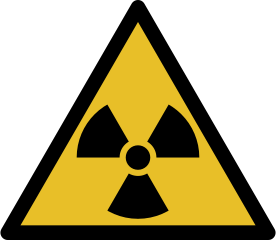
\includegraphics[width=0.75\linewidth]{images/radioactive.png}%
\\[\jot]\footnotesize\flushleftright\color{mpcolor}%
When we see this symbol we know that there's matter that's only balanced, not conserved -- which involves danger%
}%

\nonosection{Examples of applications}
\label{nsec:matter_applic}

\nonosubsection{Rigid-body and particle mechanics}
\label{nsec:cons_matter_particle}

In many applications we set up our description of the physical phenomenon of interest in such a way that the law of conservation of matter is automatically satisfied. This is achieved by choosing a sequence of closed control surfaces for which the flux of matter is zero, and therefore the amount of matter in the control volumes is constant. This procedure is often carried without many comments -- to the point of being almost forgotten at times.

We saw an example of this procedure in the {numerical evolution of the motion of a falling object}.
\marginpar{\centering%
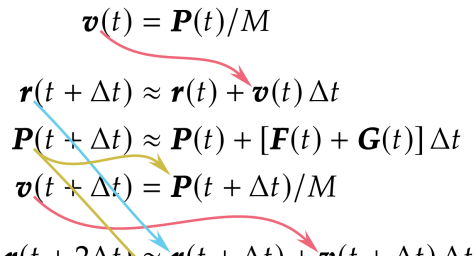
\includegraphics[align=t,width=\linewidth]{images/timesteps.png}%
\\[2\jot]\footnotesize\color{mpcolor}%
Snippet of formula~\eqref{eq:timestep_momentum_position}%
}%
Take again a look at the timesteps in formula~\eqref{eq:timestep_momentum_position}: you see that at each timestep we calculate the velocity $\yv$ of matter from the momentum $\yP$, simply dividing by the mass $\yM$. \emph{This mass is assumed to be constant, not changing with time}. But this mass is proportional to the amount of matter: $\yM = \yrho \yN$. We are therefore assuming that the amount of matter $\yN$ doesn't change with time: $\di\yN(t)/\di t = 0$. This assumption is indeed guaranteed by the balance of matter~\eqref{neq:cons_matter}, by choosing a sequence of control surfaces that have no net flux of matter through them: $\yJ(t)=0$; in other words, they tightly wrap and follow the moving object.


\nonosubsection{Chemistry}
\label{nsec:cons_matter_chemistry}

One of the main assumptions in chemistry is the \enquote*{permanence of atoms}. This assumption imposes important restrictions in the \furl{https://doi.org/10.1351/goldbook.S06026}{stoichiometry} of chemical reactions, that is, in determining the amounts of products that can appear from given amounts of reactants.
\marginpar{\centering%
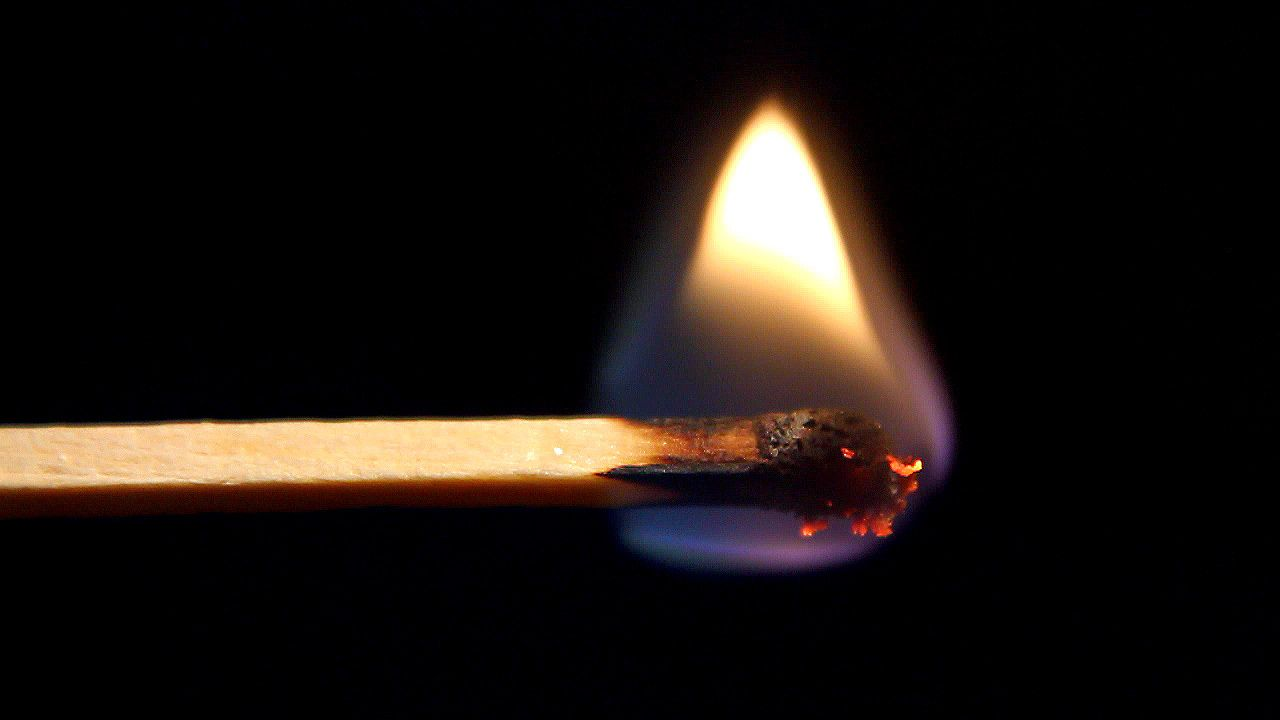
\includegraphics[align=t,width=\linewidth]{images/match_reaction.jpg}%
% \\[2\jot]\footnotesize{\color{mpcolor}%
% A match burning}%
}%
For instance, the \furl{https://chem.washington.edu/lecture-demos/match-head-reaction}{match-head reaction}
\begin{equation*}
  3\,\mathrm{P_{4}} + 10\,\mathrm{K\,Cl\,O_{3}}
  \to 3\,\mathrm{P_{4}O_{10}} + 10\,\mathrm{K\,Cl}
  % \mathrm{CH_{3}CHO} \to \mathrm{CH_{4}} + \mathrm{CO}
\end{equation*}
expresses that if 30 moles of oxygen (O) atoms appear among the reactants, they must also appear among the products; same for the 12 moles of \furl{https://pubchem.ncbi.nlm.nih.gov/element/Phosphorus}{phosphorus (P) atoms}, the 10 moles of \furl{https://pubchem.ncbi.nlm.nih.gov/element/Potassium}{potassium (K) atoms}, and so on.

This assumption is simply the statement of conservation of matter, \emph{separately} for each chemical element: since the reaction doesn't let any other matter go in or out, the flux $\yJ$ for each chemical element must be zero. Therefore the amount $\yN$ of each chemical element must be constant: $\di\yN(t)/\di t = \yJ = 0$.

This assumption is often called \enquote*{conservation of mass}, but, as previously explained, \autoref{nsec:cons_matter_formulation}{\enquote{mass} is in this case only a proxy for matter}. The assumption of the permanence of atoms is only approximate and no longer valid in phenomena for which nuclear physics or particle physics become relevant.

\nonosubsection{Climate}
\label{nsec:cons_matter_climate}

The laws of conservation and balances of matter turn out to be very useful also in problems related to climate.

On the Earth's surface and atmosphere we can assume a law of conservation of matter for each of the \furl{https://www.britannica.com/science/isotope/The-discovery-of-isotopes\#ref496311}{stable isotopes} of the chemical elements, for instance the \furl{https://education.jlab.org/itselemental/ele006.html}{two stable carbon isotopes} and the \furl{https://education.jlab.org/itselemental/ele008.html}{three stable oxygen isotopes}. We can therefore follow these isotopes as they flow between different physical systems, like the atmosphere, the oceans, and the biosphere, especially plants -- in practice we are using huge control volumes.

For the radioactive isotopes, the \autoref{sec:matter_const_radioactive}{law of radioactive decay} applies, and from it we can deduce the age of different materials and objects like ice or wood.

% %
% \marginpar{\centering%
% 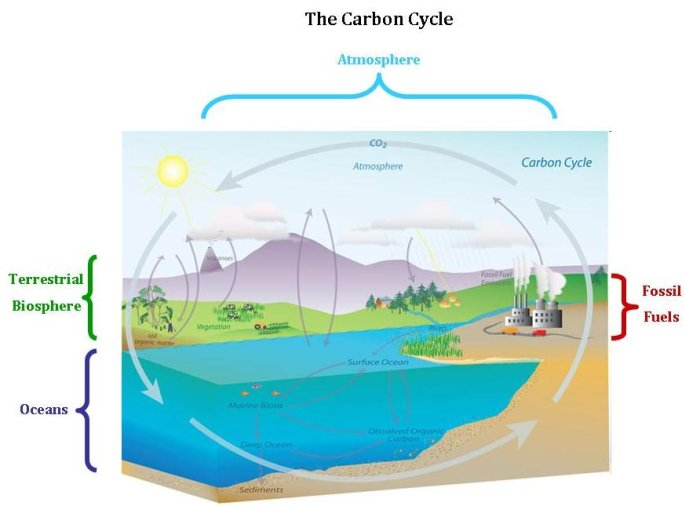
\includegraphics[align=t,width=\linewidth]{images/carbon_cycle.jpg}%
% \\[2\jot]\footnotesize\flushleftright{\color{mpcolor}%
%   The fluxes of carbon across the \enquote*{control volumes} of atmosphere, oceans, and other environments (image from \furl{https://gml.noaa.gov/outreach/isotopes/}{Global Monitoring Laboratory})}%
% }%
This is how we are able to say that human usage of fossil fuel is an important factor in the increase of carbon dioxide ($\mathrm{CO_{2}}$) in the atmosphere during the past 200 years or so. Take a look at the more detailed explanations given by the \furl{https://gml.noaa.gov/outreach/isotopes/}{Global Monitoring Laboratory}.

%
\marginpar{\vspace{2\baselineskip}\centering%
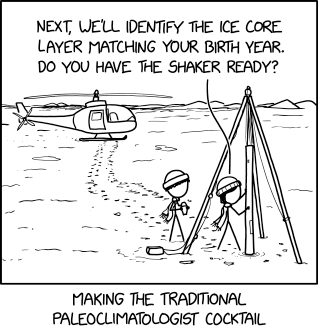
\includegraphics[width=\linewidth]{images/ice_core.png}%
\\\footnotesize\color{mpcolor}\url{https://xkcd.com/2902}%
}%
\begin{exercise}
  Measuring the relative amounts of carbon within an air pocket near the surface of a block of ice, you find that one mole of air contains \qty[print-unity-mantissa=false]{1e-12}{mol} of the radioactive isotope \nuclide[14]{C}. Making an analogous measurement for an air pocket deeper in the ice, you find instead a relative abundance of \qty{2e-13}{mol} of \nuclide[14]{C}. How old is the deeper section of ice?

  Find out the ice's age $t_{\text{ice}}$ by numerically evolving the balance equation
  $$\frac{\di\yN(t)}{\di t} = -\lambda\,\yN(t)$$
  with $\lambda=\qty{0.000122}{yr^{-1}}$, until you reach the amount $\yN(t_{\text{ice}})= \qty{2e-13}{mol}$.
  Use the procedure of \autoref{sec:numeric_simulation}{\eqn~\eqref{eq:finite_diff}}, starting from time $\yti=\qty{0}{yr}$ and $\yN(\yti)=\qty[print-unity-mantissa=false]{1e-12}{mol}$, and assuming that the flow $\yJ(t)$ of \nuclide[14]{C} is zero. You can use a timestep $\Dt = (1/365)\:\unit{yr}$.
\end{exercise}


\nonosubsection{Fluid dynamics}
\label{nsec:fluid_dyn_areavel}

The law of conservation of matter in its explicit form is at the heart of fluid-dynamic problems. Consider the flow of a fluid (liquid or gas) for instance through a pipe or through a jet engine. When we say that a flow is \textbf{steady} we mean that the volume contents and the fluxes taken for whatever control volumes and surfaces do not change in time (though they may change in space). This condition can be viewed as a constitutive relation.

%
\marginpar{\vspace{-\baselineskip}\centering%
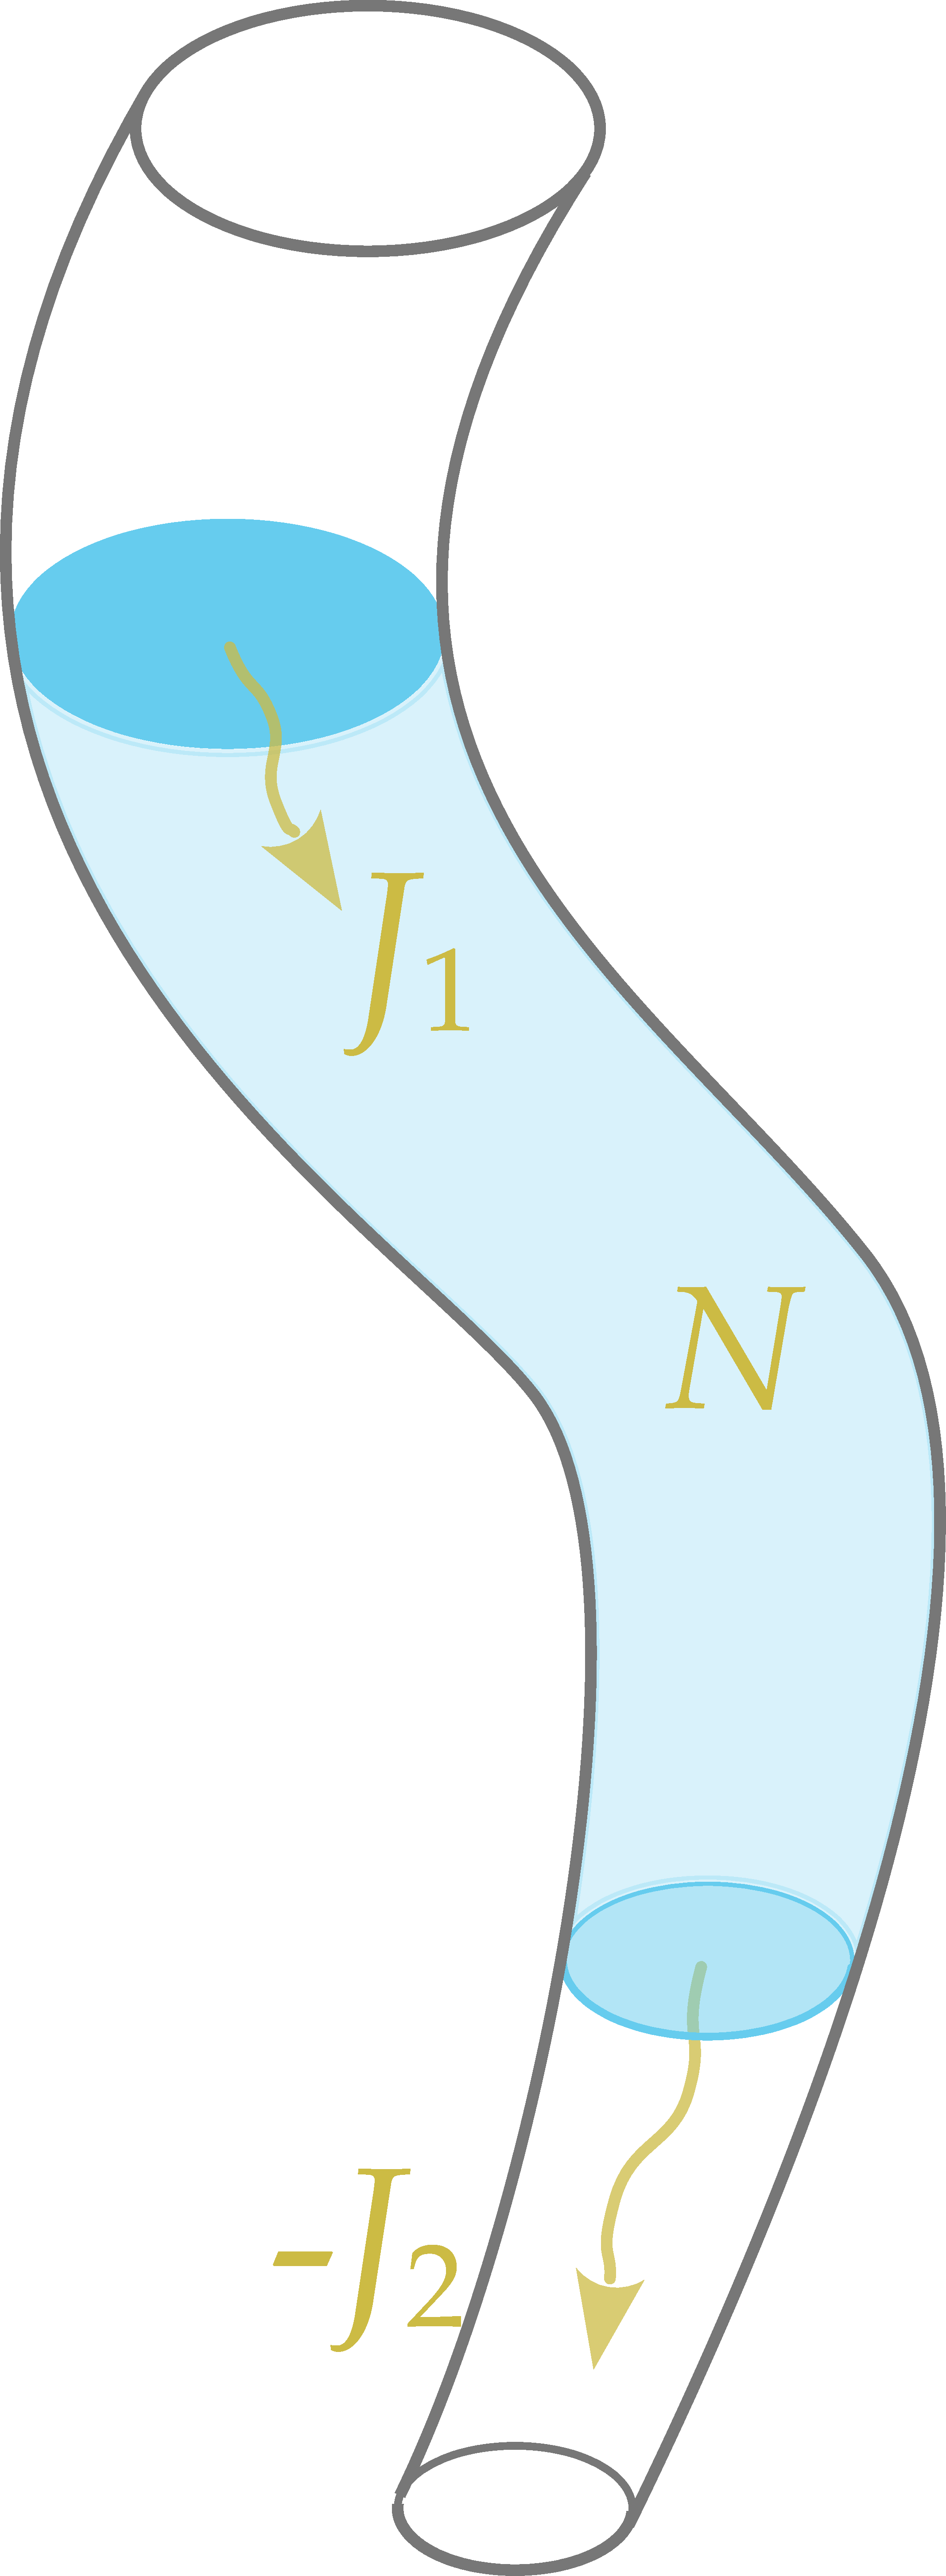
\includegraphics[height=15em]{images/pipesection.pdf}%
}%
Consider a control volume, for instance the one indicated in \textcolor{cyan}{light blue} in the side picture. The amount of fluid $\yN$ in this volume is constant in time: $\frac{\di\yN(t)}{\di t}=0$. By the law of conservation of matter, the total influx must then be zero:
\begin{equation*}
  {\color{grey}\underbrace{\color{black}\frac{\di\yN(t)}{\di t}}_{\color{grey}{}=0}\color{black}} - \yJ(t) = 0
  \qquad\Longrightarrow\qquad
  \yJ(t) = 0
\end{equation*}
and it is given by the influxes through three surfaces: the side surface, the one at the top, and the one at the bottom. The influx through the side surface is zero. Let us denote the influx through the top surface by $\yJ_{1}$, and the influx through the bottom surface by $\yJ_{2}$. We must therefore have
\begin{equation*}
  0 = \yJ(t) = \yJ_{1}(t) + \yJ_{2}(t)
  \qquad\Longrightarrow\qquad
  \yJ_{1}(t) = -\yJ_{2}(t)
\end{equation*}
%
\marginpar{\centering%
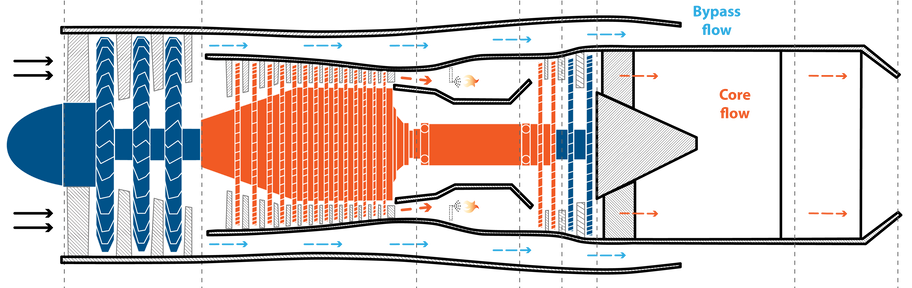
\includegraphics[align=t,width=\linewidth]{images/jet1.png}%
\\[\jot]\footnotesize\color{mpcolor}%
(image from \furl{https://www.jet-x.org/a8.html}{JetX})%
}%
that is, the influx through the top surface must equal the efflux through the bottom one.
This is a very powerful deduction: consider that it is valid even if the flow of the fluid is turbulent, and it is valid in more general situations such as at different sections of a jet engine.

\medskip

If the surfaces are small enough, we can also use the {connection between flux and velocity}:
\begin{equation*}
  v_{1} = \frac{\yJ_{1}/A_{1}}{\yN/V}
  \qquad
  v_{2} = \frac{-\yJ_{2}/A_{2}}{\yN/V}
\end{equation*}
where $A_{1}, A_{2}$ are  the areas  of the top and bottom surfaces, and $v_{1}, v_{2}$ the \emph{downward} velocities through them (hence the minus sign for the bottom surface). From $\yJ_{1} = -\yJ_{2}$ we then find this important relationship:
\begin{equation*}
  v_{1}\,A_{1} = v_{2}\,A_{2}
\end{equation*}
that is, if the area through which the flux occur decreases, then the velocity of the fluid through it increases, and vice versa.
%
\marginpar{\vspace{-7\baselineskip}\centering%
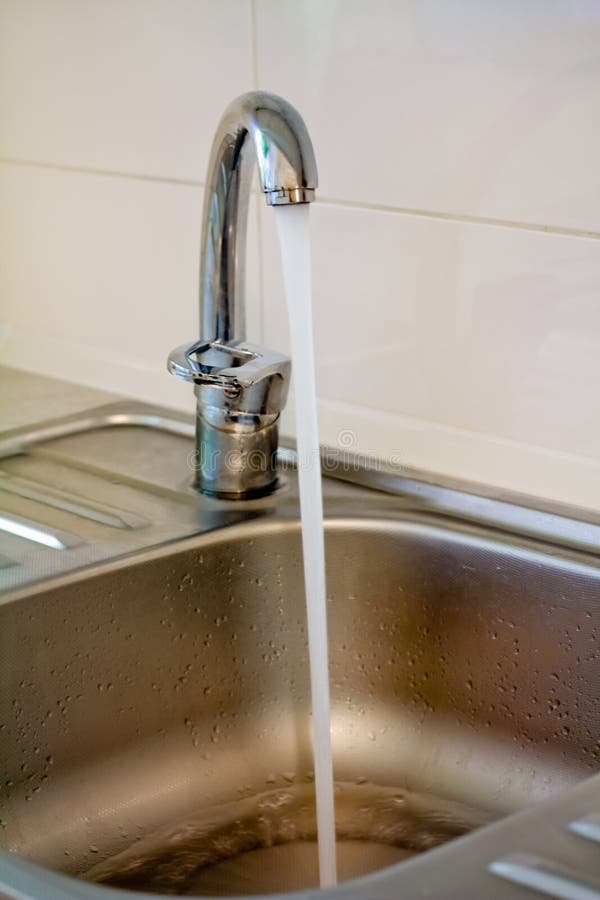
\includegraphics[width=0.5\linewidth]{images/tap_water.jpg}%
\\[\jot]\footnotesize\flushleftright\color{mpcolor}%
The thickness and velocity variations of tap water are a consequence of the law of conservation of matter%
}%
This is  what we often observe in running water from our taps.

\bigskip



%%%***venturi tube


\printpagenotes*
\clearpage
\nonochapter{Balance of energy}
\label{ncha:bal_energy}

\printpagenotes*
\clearpage
\nonochapter{Balance of momentum}
\label{ncha:bal_momentum}

\epigraph{\emph{%
I hold in fact
 \begin{enumerate}[label=(\arabic*),wide,itemindent=2em]
 \item That small portions of space \emph{are} in fact of a nature analogous to little hills on a surface which is on the average flat; namely, that the ordinary laws of geometry are not valid in them.
 \item That this property of being curved or distorted is continually being passed on from one portion of space to another after the manner of a wave.
 \item That this variation of the curvature of space is what really happens in that phenomenon which we call the \emph{motion of matter}, whether ponderable or etherial.
 \item That in the physical world nothing else takes place but this variation, subject (possibly) to the law of continuity.
 \end{enumerate}
}}{W. K. Clifford \cites*{clifford1876}}


\printpagenotes*
\clearpage
\nonochapter{Balance of angular momentum}
\label{ncha:bal_ang_momentum}

% \printpagenotes*
% \clearpage
% \nonochapter{Conservation of electric charge and magnetic flux}
% \label{ncha:cons_charge_magneticflux}
%
% \printpagenotes*
% \clearpage
% \nonochapter{Balance of entropy}
% \label{ncha:bal_entropy}





\smallskip


\printpagenotes*
\clearpage
\nonochapter{Densities and flux-densities}
\label{ncha:density_fluxdensity}


How do we mathematically represent the seven main quantities? We said that, for each, we can ask \emph{how much in this region?} and \emph{how much through this surface during this time?} We must therefore use mathematical objects that allow us to answer these two questions. These objects are the \emph{density} and the \emph{flux vector}. The idea behind them is quite simple.
%Let us take the quantity \emph{matter} as an example.


\begin{definition}{Density}
  Take a point in spacetime with coordinates $(\yti,\yxi,\yyi,\yzi)$. At the instant $\yti$, imagine a very small cuboid centred at $(\yxi,\yyi,\yzi)$, with sides aligned with the coordinate axes $x,y,z$ and of lengths $\Dx$, $\Dy$, $\Dz$. Then we have
  \begin{equation}
    \label{neq:density_expl}
    \text{\small amount of quantity in cuboid} =
    n(\yti,\yxi,\yyi,\yzi)\, \Dx\, \Dy\, \Dz \ .
  \end{equation}
  where $n(\yti,\yxi,\yyi,\yzi)$ is the \textbf{density} at the spacetime point $(\yti,\yxi,\yyi,\yzi)$.
\end{definition}
The density tells us how much quantity there's in a unit of volume. As the notation suggests, it is a function of the coordinates, that is, of time and spatial position. This functional dependence reflects the fact that we can have a larger amount of a quantity concentrated in some regions at some times, than in other regions or at other times.

In order to calculate the total amount of the quantity in an arbitrary 3D region, we simply divide it into very small cuboids similar to the one above. For each cuboid we calculate the respective amount; this amount will generally be different from cuboid to cuboid, because the value of the density $n(t,x,y,z)$ will be different at each cuboid's centre. Then we sum up all these amounts.

\begin{extra}{Isn't this an integral?}
  You probably recognize this procedure as the description of integration. Indeed we can write:
  \begin{equation}
    \label{neq:density_integral}
    \text{\small total amount of quantity in 3D region} =
    \iiint\limits_{\mathclap{\text{3D region}}}n(t,x,y,z)\, \di x\, \di y\, \di z \ .
  \end{equation}
\end{extra}
Clearly we must know the value of the density $n$ at all points within the region, in order to calculate the total amount. Note that if the quantity is absent in some subregion, then $n(\dotso)=0$ there.

\medskip


\begin{warning}[Do not confuse flux with movement]
  Flux
\end{warning}

For the flux of the quantity through a surface we consider three different cases:
\begin{definition}{$x$-Flux}
  Take again a point in spacetime with coordinates $(\yti,\yxi,\yyi,\yzi)$. Keeping $\yxi$ fixed, imagine a very small rectangular surface centred at $(\yxi,\yyi,\yzi)$, with sides aligned with the coordinate axes $y,z$ and of lengths $\Dy$, $\Dz$. Imagine that this surface exists for a lapse of time $\Dt$ around the time $\yti$. Then we have
  \begin{equation}
    \label{neq:xflux_expl}
    \left.\parbox[c]{10em}{\small amount of quantity\\ through rectangle $\Dy\,\Dz$\\ towards positive $x$\\during time lapse }\right\} =
    j_{x}(\yti,\yxi,\yyi,\yzi)\, \Dt\, \Dy\, \Dz \ .
  \end{equation}
  where $j_{x}(\yti,\yxi,\yyi,\yzi)$ is the \textbf{$x$-flux} at the spacetime point $(\yti,\yxi,\yyi,\yzi)$.
\end{definition}
The $x$-flux tells us how much quantity is flowing in a unit of time through a unit of surface parallel to $y,z$. Also the $x$-flux is a function of the coordinates, because the flux could be larger through some surfaces at some times, than through other surfaces at other times. If the quantity is flowing in the negative $x$ direction, then $j_{x}$ will be negative; and clearly if no quantity is flowing through the small rectangle, then $j_{x}=0$.

In an analogous way we define a $y$-flux and a $z$-flux:

\begin{definition}{$y$-Flux}
  \begin{equation}
    \label{neq:yflux_expl}
    \left.\parbox[c]{10em}{\small amount of quantity\\ through rectangle $\Dz\,\Dy$\\ towards positive $y$\\during time lapse }\right\} =
    j_{y}(\yti,\yxi,\yyi,\yzi)\, \Dt\, \Dz\, \Dy \ .
  \end{equation}
\end{definition}
\begin{definition}{$z$-Flux}
  \begin{equation}
    \label{neq:zflux_expl}
    \left.\parbox[c]{10em}{\small amount of quantity\\ through rectangle $\Dx\,\Dy$\\ towards positive $z$\\during time lapse }\right\} =
    j_{z}(\yti,\yxi,\yyi,\yzi)\, \Dt\, \Dx\, \Dy \ .
  \end{equation}
\end{definition}

The three fluxes can be grouped into the \textbf{flux vector}
\begin{equation}
  \label{neq:flux_vector}
  \bm{j}(t,x,y,z) \defd
  \bigl(j_{x}(t,x,y,z),\ j_{y}(t,x,y,z),\ j_{z}(t,x,y,z)\bigr)
\end{equation}

In order to calculate the total amount of the quantity through an arbitrary sequence of 2D surfaces during a time lapse, we simply divide the total time into very brief time lapses, and for each of these we approximate the surface with very small rectangles aligned along the three axes. For each such lapse and rectangle we calculate the respective flux amount, using $j_{x}$, $j_{y}$, or $j_{z}$ depending on the orientation of the rectangle. Then we sum up all these amounts.
\begin{extra}
  This is also the description of an integration, which can be written
  \begin{multline}
    \label{neq:flux_integral}
    \text{\small total amount of quantity through sequence of surfaces} = {}\\
    \begin{multlined}[b][0.9\linewidth]
      \iiint j_{x}(t,x,y,z)\, \di t\, \di y\, \di z +{}
      \\\iiint j_{y}(t,x,y,z)\, \di t\, \di z\, \di y +{}
      \\\iiint j_{z}(t,x,y,z)\, \di t\, \di x\, \di y
    \end{multlined}
  \end{multline}

  We shall not have to calculate density integrals~\eqref{neq:density_integral} and flux integrals~\eqref{neq:flux_integral} in these notes. In concrete physics problems these integrals are often difficult to calculate, and require advanced mathematical techniques and specialized software. But if you'll ever end up working in fields like computational fluid dynamics, atmospheric or ocean modelling, or numerical relativity, then you shall probably encounter them again.
\end{extra}

\medskip

The definitions above of density and flux are appropriate if the quantity in question is a scalar. For vector quantities like momentum and angular momentum, the density is a vector, and each of the three fluxes is a vector as well.
% For instance, for matter we could have $\yN(\yti)=\qty{3.5}{mol}$, and for energy we could have $\yJ=\qty{-600}{J}$. For momentum and angular momentum, each of the three amounts is instead a vector, of appropriate physical dimensions, that can have any magnitude and direction or components. For instance, for momentum we could have $\bm{N}_{2} = (-3.4,0,+5)\,\unit{kg\cdot m/s}$.

%% ***
% The flux tells us how much quantity is flowing through a unit of surface in a unit of time. Density and flux can change from spacetime point to spacetime point. We shall discuss them more in detail for each quantity later on. One important aspect to keep in mind is that \emph{the density and flux of each quantity depend on the coordinate system}.



\nonosection{Balance laws expressed with derivatives}
\label{nsec:balance_derivative}

In \chap\,\ref{ncha:density_fluxdensity} we saw that each of the main seven quantities is represented by a density and by a flux vector, which allow us to calculate the amount of quantity within a 3D region at a particular time, an flowing through a 2D surface during an time interval. These amounts are exactly what $\yN(\yti)$, $\yN(\ytf)$, $\yJ$ express. Therefore, a conservation or balance law must also give some relationship between density and flux vector.

The way to find such relationship is intuitive and mathematically simple, if only a bit lengthy. The idea is to formulate the balance law for a very simple case, the same simple set-up that we used in \chap\,\ref{ncha:density_fluxdensity} to introduce density and flux.

Take a point in spacetime with coordinates $(t,x,y,z)$. We apply the conservation law~\eqref{eq:conserved} to the following situation:
\begin{itemize}
\item[$\yN(\yti)$:] Choose an initial time $\yti=t-\Dth$, slightly before $t$, and a cuboid region centred at $(x,y,)$ with sides $\Dx$, $\Dy$, $\Dz$. The total amount of the quantity within this region is given, adapting formula~\eqref{neq:density_expl}, by
  \begin{equation}
    \label{neq:C1dens}
    \yN(\yti) = n\bigl(t-\Dth, x,y,z\bigr)\,\Dx\,\Dy\,\Dz \ .
  \end{equation}

\item[$\yN(\ytf)$:] Choose a final time $\ytf = t+\Dth$, slightly after $t$, and a cuboid region centred at $(x,y,)$ with sides $\Dx$, $\Dy$, $\Dz$. The total amount of the quantity within this region is given, adapting formula~\eqref{neq:density_expl}, by
  \begin{equation}
    \label{neq:C2dens}
    \yN(\ytf) = n\bigl(t+\Dth, x,y,z\bigr)\,\Dx\,\Dy\,\Dz \ .
  \end{equation}

\item[$\yJ$:] We calculate the flux separately through the six rectangular surfaces bounding the small cuboid region:
  \begin{itemize}
  \item[$\yJ_{x}$:] First choose a rectangular surface centred slightly to one side of the point $(x,y,z)$: at $(x-\Dxh, y, z)$, with sides parallel to $y,z$ and lengths $\Dy, \Dz$. We keep this surface constant for the small duration $\Dt$. The $x$-flux through this rectangle, towards positive $x$, during $\Dt$, is according to formula~\eqref{neq:xflux_expl}
    \begin{equation*}
      \label{neq:Fxfluxn}
     \yJ_{x}^{\text{in}} = j_{x}\bigl(t, x-\Dxh, y, z\bigr)\,\Dt\,\Dy\,\Dz \ .
    \end{equation*}
    Now choose the rectangular surface parallel to the previous one, but on the other side of the point $(x,y,z)$, centred at $(x+\Dxh, y, z)$. The $x$-flux through this rectangle, towards positive $x$, during $\Dt$, is
    \begin{equation*}
      \label{neq:Fxfluxp}
      \yJ_{x}^{\text{out}} = j_{x}\bigl(t, x+\Dxh, y, z\bigr)\,\Dt\,\Dy\,\Dz \ .
    \end{equation*}
    Note that the flux $\yJ_{x}^{\text{in}}$ points to the interior of the 3D region, towards its centre $(x,y,z)$; whereas $\yJ_{x}^{\text{out}}$ points to the exterior, away from the centre. The total flux into the region is therefore given by their difference:
    \begin{equation}
      \label{neq:Fxflux}
      \begin{split}
        \yJ_{x} &= \yJ_{x}^{\text{in}} - \yJ_{x}^{\text{out}}
        \\&= \bigl[ j_{x}\bigl(t, x-\Dxh, y, z\bigr) - j_{x}\bigl(t, x+\Dxh, y, z\bigr)\bigr]
        \,\Dt\,\Dy\,\Dz
      \end{split}
    \end{equation}

  \item[$\yJ_{y}, \yJ_{z}$:] An analogous reasoning can be made to find the total flux through the other four surfaces, two parallel to $z,y$ and two to $x,y$. We find
    \begin{align}
      \label{neq:Fyflux}
      \begin{split}
        \yJ_{y} &= \yJ_{y}^{\text{in}} - \yJ_{y}^{\text{out}}
        \\&= \bigl[ j_{y}\bigl(t, x, y-\Dyh, z\bigr) - j_{x}\bigl(t, x, y+\Dyh, z\bigr)\bigr]
        \,\Dt\,\Dz\,\Dx
      \end{split}
      \\[3\jot]
      \label{neq:Fzflux}
      \begin{split}
        \yJ_{z} &= \yJ_{z}^{\text{in}} - \yJ_{z}^{\text{out}}
        \\&= \bigl[ j_{z}\bigl(t, x, y, z-\Dzh\bigr) - j_{x}\bigl(t, x, y, z+\Dzh\bigr)\bigr]
        \,\Dt\,\Dx\,\Dy
      \end{split}
    \end{align}
  \end{itemize}
The total flux into the region during the time interval $\Dt$ is finally the sum of the three above:
\begin{equation}
  \label{neq:Fflux}
  \yJ = \yJ_{x} + \yJ_{y} + \yJ_{z}
\end{equation}
\end{itemize}

Up to now we have only chosen arbitrary surfaces, regions, and a time interval. Now let's assume that the corresponding amounts and fluxes satisfy a balance law like~\eqref{eq:conserved}. Putting together the puzzle pieces we find
\begin{multline*}
  \label{neq:balance_pieces}
    \mathcolor{blue}{\yN(\ytf)} -\mathcolor{green}{\yN(\yti)} - \mathcolor{red}{\yJ} = 0 \qquad     \Longrightarrow
    \\[2\jot]
    \left.\begin{aligned}
      &\mathcolor{blue}{n\bigl(t+\Dth, x,y,z\bigr)\,\Dx\,\Dy\,\Dz}
      - \mathcolor{green}{n\bigl(t-\Dth, x,y,z\bigr)\,\Dx\,\Dy\,\Dz}
      \\[\jot]\quad&\color{red}-\bigl[ j_{x}\bigl(t, x-\Dxh, y, z\bigr) - j_{x}\bigl(t, x+\Dxh, y, z\bigr)\bigr]
      \,\Dt\,\Dy\,\Dz
      \\[\jot]\quad&\color{red}-\bigl[ j_{y}\bigl(t, x, y-\Dyh, z\bigr) - j_{x}\bigl(t, x, y+\Dyh, z\bigr)\bigr]
      \,\Dt\,\Dz\,\Dx
      \\[\jot]\quad&\color{red}-\bigl[ j_{z}\bigl(t, x, y, z-\Dzh\bigr) - j_{x}\bigl(t, x, y, z+\Dzh\bigr)\bigr]
      \,\Dt\,\Dx\,\Dy
    \end{aligned}\enspace\right\}=0
\end{multline*}
This expression is quite long, but it should be intuitively understandable if you try to identify the individual summed terms.

Now we take the last, long expression -- which is an equality -- and divide its left and right sides by $\Dt\,\Dx\,\Dy\,\Dz$. Note that many of the \enquote{$\incr$} factors simplify out. We arrive at this:
\begin{equation*}
  \label{neq:balance_deriv_incr}
  \left.\begin{aligned}
      &\frac{n\bigl(t+\Dth, x,y,z\bigr)
      -n\bigl(t+\Dth, x,y,z\bigr)}{\Dt}
      \\[\jot]\quad&+\frac{j_{x}\bigl(t, x+\Dxh, y, z\bigr) - j_{x}\bigl(t, x-\Dxh, y, z\bigr)}{\Dx}
      \\[\jot]\quad&+\frac{j_{y}\bigl(t, x, y+\Dyh, z\bigr) - j_{y}\bigl(t, x, y-\Dyh, z\bigr)}{\Dy}
      \\[\jot]\quad&+\frac{j_{z}\bigl(t, x,y,z+\Dzh\bigr) - j_{z}\bigl(t, x,y,z-\Dzh\bigr)}{\Dz}
    \end{aligned}\enspace\right\}=0 \ .
\end{equation*}
Still a long expression; but examine each fraction: we have a difference between a term calculated at some point, and one calculated at some point plus an increment \enquote{${}\incr$}; this difference is then divided by that increment. This is the definition of \emph{partial derivative}, that is, the derivative with respect to one variable, while keeping the other variables fixed. The short symbol for this is \enquote{$\frac{\de\dotso}{\de\dotso}$}, so we can simply write
\begin{definition}{Conservation law in derivative form}
  \begin{equation}
    \label{neq:balance_deriv}
    \frac{\de n}{\de t}%(t,x,y,z)
    +\frac{\de j_{x}}{\de x}%(t,x,y,z)
    +\frac{\de j_{y}}{\de y}%(t,x,y,z)
    +\frac{\de j_{z}}{\de z}%(t,x,y,z)
    = 0
  \end{equation}
\end{definition}
Let's make a simple check to see if this formula makes sense, in a simple one-dimensional case where we disregard the $y,z$ coordinates (let's say their fluxes are zero), so that the balance law becomes
\begin{equation*}
  \frac{\de n}{\de t} + \frac{\de j_{x}}{\de x} = 0 \ .
\end{equation*}
\marginpar{\footnotesize%
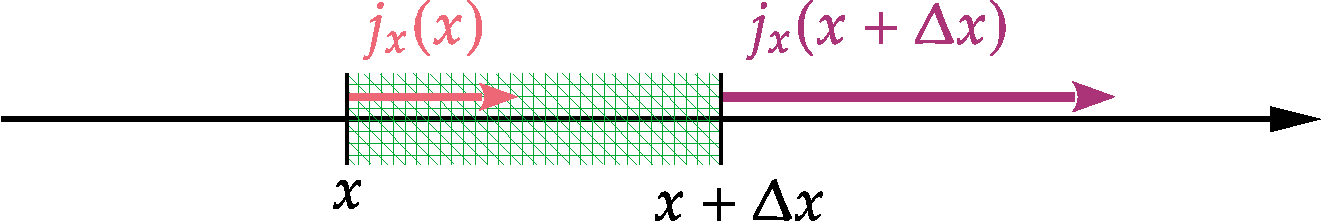
\includegraphics[align=t,width=\linewidth]{images/ddxflux.pdf}
}
Suppose that the derivative of the $x$-flux is positive: $\frac{\de j_{x}}{\de x} > 0$. This means that the $x$-flux increases as we move from $x$ to $x+\Dx$, as shown in the side figure. The $x$-flux at $x$ is bringing some amount of quantity into the region of interest, the $x$-flux at  $x+\Dx$ is taking a larger amount out of that region. Therefore, during the short time $\Dt$ in which this flux takes place, the total amount of quantity within the region will decrease. But the total amount is given by $n(t)$, which is therefore decreasing with time. This means that its time derivative is negative: $\frac{\de n}{\de t} < 0$. This agrees with balance law above: the sum of the two derivatives must be zero, so if one is positive, the other must be negative.

\medskip

Balance laws like~\eqref{neq:balance_deriv} are the basis of many important computational and simulation methods in a huge variety of physical applications: simulation of the ocean around an offshore oil platform, of wind in a wind farm, of air around an aeroplane's wing, of earthquakes, of electromagnetic-wave propagation, of oscillations in a suspension bridge, of percolation of fluids through terrain, of chemical reactions, of energy transfer\textellipsis The list could go on for pages!

The basic idea for using a balance law for a simulation is easy to understand. Take again the simpler one-dimensional formula without $y,z$ coordinates, and rewrite it remembering the basic meaning of the derivative:
\begin{equation*}
  \frac{n(t+\Dt,x)-n(t,x)}{\Dt} + \frac{j_{x}(t, x+\Dxh)-j_{x}(t,x-\Dxh)}{\Dx} = 0
\end{equation*}
Suppose we know all quantities at time $t$; we can then find the density $n$ at time $t+\Dt$. Leave it on the left side and bring all other terms on the right side, multiplying them by $\Dt$:
\begin{equation*}
  n(t+\Dt,x) =
  \Dt\,\biggl[ n(t,x) - \frac{j_{x}(t, x+\Dxh)-j_{x}(t,x-\Dxh)}{\Dx} \biggr]
\end{equation*}
which is essentially \furl{https://mathworld.wolfram.com/EulerForwardMethod.html}{Euler's method}.

This formula can then be used iteratively to find the density $n$ at later times. As a simple simulation set-up, we consider a region of space of interest and divide it into cells of width $\Dx$. We also treat time in steps of $\Dt$. Then the iterative procedure goes as follows:
\begin{myframe}
  \begin{enumerate}[label=\arabic*.,ref=\arabic*]
  \item \emph{Initial values:} Assign the value of $n$ at each $x$-cell at the initial time.
  \item\label{nitem:timestep} \emph{For-loop in $x$:} for each $x$-cell, calculate the value of $n$ at $t+\Dt$, using the formula above.
  \item Increase time by $\Dt$.
  \item Go to~\ref{nitem:timestep}.
  \end{enumerate}
\end{myframe}

For example, suppose we have two $x$-cells of width $\Dx=1$: one centred at $x_{1}$ and the other at $x_{2} = x_{1}+1$. There are three boundaries: the leftmost at $x_{1}-\tfrac12$, one between the cells at $x_{1}+\tfrac12 \equiv x_{2}-\tfrac12$, and the rightmost at $x_{2}+\tfrac12$. Then we have the following steps:

{\small

\begin{enumerate}[label=\arabic*.]
\item Assign the values $n(\yti,x_{1}), n(\yti,x_{2})$ of $n$ at $x_{1}$ and $x_{2}$ at time $\yti$.

\item Assign the values $$j_{x}\bigl(\yti,x_{1}-\tfrac12\bigr)\ , \enspace j_{x}\bigl(\yti,x_{1}+\tfrac12\bigr)\ , \enspace j_{x}\bigl(\yti,x_{2}+\tfrac12\bigr)$$
  of the fluxes at the three boundaries at time $\yti$.

\item Calculate the values of $n$ at $x_{1}$ and $x_{2}$ at time $\yti=\yti+\Dt$, for instance
  $$ n(\yti,x_{1}) =
  \Dt\,\biggl[ n(\yti,x_{1}) - \frac{j_{x}(\yti, x_{1}+\tfrac12)-j_{x}(\yti,x_{1}-\tfrac12)}{\Dx} \biggr] \ .$$
  Note that we have all quantities required on the right side.

\item Assign the values $$j_{x}\bigl(\yti,x_{1}-\tfrac12\bigr)\ , \enspace j_{x}\bigl(\yti,x_{1}+\tfrac12\bigr)\ , \enspace j_{x}\bigl(\yti,x_{2}+\tfrac12\bigr)$$
  of the fluxes at the three boundaries at time $\yti$.

\item Calculate the values of $n$ at $x_{1}$ and $x_{2}$ at time $\ytf=\yti+\Dt$, for instance
  $$ n(\ytf,x_{1}) =
  \Dt\,\biggl[ n(\yti,x_{1}) - \frac{j_{x}(\yti, x_{1}+\tfrac12)-j_{x}(\yti,x_{1}-\tfrac12)}{\Dx} \biggr] \ .$$
  Note that we have again all quantities required on the right side.

\item And so on.
\end{enumerate}

}

This routine requires us \emph{to know the flux at each $x$-cell and at each time}. But we shall soon see that this requirement can be bypassed.

The rudimentary routine above is the basis from which more precise and complex simulation routines are developed.

\begin{exercise}
  Write a script, in your preferred programming language, that implements the simulation routine above in an $x$-grid with four cells $x=1,\ \dotsc,\ x=4$. Take a grid size $\Dx=1$ and time step $\Dt=1$. We can imagine that the quantity in question is electric charge. Use the following initial values for $n(t,x)$ at $t=0$:
  \begin{equation*}
    n(t\mo0, x\mo1)=7\ ,\enspace
    n(t\mo0, x\mo2)=0\ ,\enspace
    n(t\mo0, x\mo3)=0\ ,\enspace
    n(t\mo0, x\mo4)=7
  \end{equation*}
  and assume the flux is, at each time $t$:
  \begin{multline*}
      j_{x}(t, x\mo0.5)=0\ ,\\
      j_{x}(t, x\mo1.5)=+2\ ,\enspace
      j_{x}(t, x\mo2.5)=0\ ,\enspace
      j_{x}(t, x\mo3.5)=-2\ ,\\
      j_{x}(t, x\mo4.5)=0 \ .
    \end{multline*}

    Questions and tasks:
    \begin{enumerate}[exerc]
    \item Which time evolution for $n$ do you observe? Does it make sense, given the fluxes above?
    \item Feel free to try out or generalize your script with:
      \begin{itemize}[shift]
      \item different initial values
      \item different fluxes
      \item an explicit formula for the flux, for instance
        \begin{equation*}
          j_{x}(t,x) = 8\,x^{3} - 60\,x^{2} + 118\,x - 45
        \end{equation*}
      \item time-dependent fluxes
      \item more cells
      \item two or three dimensions, including $y$- or $z$-fluxes
      \end{itemize}
    \end{enumerate}

\end{exercise}



\printpagenotes*
\clearpage
\nonochapter{Matter}
\label{ncha:matter}

Matter is probably the easiest quantity to grasp intuitively; it's what we can really call \enquote{stuff}. % It is called \furl{https://doi.org/10.1351/goldbook.C01039}{\emph{chemical substance}} in chemistry, and \emph{baryons} and \emph{leptons} in particle physics.
It is important to clearly distinguish matter from \emph{mass}: mass can be considered a property of matter, but the two are different: for example, the mass of some amount of matter may change, even if the amount of matter stays the same.

There are different kinds of matter, each of which satisfies a balance relation. The distinction into different kinds depends on the physical theory. In most everyday situations, the distinction corresponds to different \furl{https://doi.org/10.1351/goldbook.C01022}{chemical elements}, and each satisfies its own balance. These balances are the basis of \furl{https://doi.org/10.1351/goldbook.S06026}{stoichiometry}. If we observe phenomena like nuclear fission or fusion, however, we notice that the balances of chemical elements are not really satisfied. With such phenomena we make a different distinction of types of matter, for instance \emph{baryons} and \emph{leptons}, and each satisfies again its own balance. It is unclear whether these balances might be broken in other physical phenomena at smaller scales. In these notes we shall usually consider chemical elements as the different kinds of matter, making some exceptions in discussion of nuclear phenomena.



\nonosection{Electric charge and magnetic flux}
\label{nsec:charge_magnetic}



\nonosection{Magnetic flux}
\label{nsec:magneticflux}

\nonosection{Energy}
\label{nsec:energy}

\nonosection{Momentum}
\label{nsec:momentum}

\nonosection{Angular momentum}
\label{nsec:rotmomentum}

\nonosection{Entropy}
\label{nsec:entropy}






%
% ** 8
% *** Structure of physical laws:
% **** fundamental
% **** constitutive
% **** boundary & initial conditions
% *** Conservation and balance laws
% *** Seven wonders of the world: geometric meaning; maths translation
% *** Why different phenomena and how to make predictions: Constitutive equations
% *** Conservation of amount of matter
% **** examples
%
% ** 9
% *** Energy: characteristics
% **** coordinate-dependent
% **** mass is energy, energy is mass
% **** matter: necessity of separation between "bulk" (mass) and small changes (energies); examples
% *** Balance of energy
% **** energy is only balanced; cosmology
%
% ** 10
% *** Momentum: characteristics
% **** coordinate-dependent
% **** momentum is energy flow, and vice versa
% **** matter: necessity of separation between "bulk" (momentum) and small changes (heat); examples
% *** Balance of momentum
% *** Force is momentum current; examples (diSessa)
%
% ** 11
% *** Angular momentum
% *** Balance of angular momentum
% *** Interlude: Conservation of charge and of magnetic flux
% *** Balance of entropy; "second law"
%
% ** 12
% *** _Special constitutive equations of Newtonian mechanics:_
% *** Momentum \propto matter flux; difference in relativity
% *** Forms of energy beside the "bulk"
% **** kinetic
% **** potential gravitational
% **** internal; several types (including chemical, elastic, etc)
% *** TODO Check work and heat
%
% ** 13
% *** _Example systems and problems_
%
% ** 14
% *** Temperature
% *** Entropy flux is (energy flux)/(temperature)
%
% ** 15
% *** Constitutive equations for internal energy: ideal gas (with dV/dt term)
% *** _Example systems and problems_
%
% ** 16
% *** Other examples: GPS?




\iffalse
\marginpar{\footnotesize%
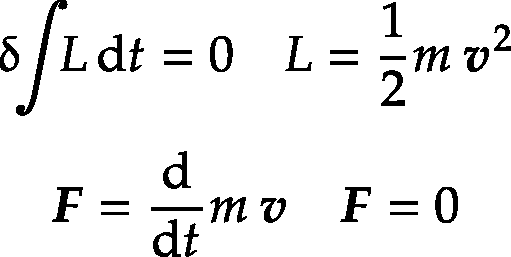
\includegraphics[align=t,width=\linewidth]{images/eg_languages.png}
\\[\jot]\color{mpcolor}\enquote{\emph{%
}}\sourceatright{\cites{}}
}
\fi




\printpagenotes*
\clearpage

\nonochapter{Thermodynamics}
\label{ncha:thermodynamics}

\nonosection{Notes on \enquote{quasi-static} processes}
\label{nsec:quasistatic}

In general, none of the statements "reversible${}\Rightarrow{}$quasi-static" or "quasi-static${}\Rightarrow{}$reversible"
is true.

A counterexample to the second implication are systems with internal state variables, which cannot be made non-dissipative, no matter how slowed-down they are. See the discussion and mathematical analysis in Astarita \sect\,2.5.


A counterexample to the first implication is a system of spins in a crystal lattice. It is possible to \emph{reversibly} bring the system form an equilibrium state to another with opposite temperature by reversing the external magnetic field \emph{as fast as possible} -- and therefore \emph{not} through a quasi-static process. In fact it is key here that the process be \emph{not}-quasi-static, but as fast as possible, because a slow change of the external magnetic field would lead to an irreversible process with dissipation. For more details see the discussion in Buchdahl, Lecture~20.

The point is that for some systems a \emph{fast} change can actually prevent the onset of dissipative phenomena, and so the process needs to be fast if we want it to be reversible. Adiabatic processes often also need to be fast (as a curious historical fact, Truesdell \amp\ Bharatha, Preface p.~xii, remark that \enquote{In introducing what we today call an `adiabatic process', Laplace called it `a sudden compression', in which he was followed by Carnot}).

In fact, clearly non-quasi-static phenomena like \emph{explosions} can in some circumstances be described by \emph{reversible} processes! This is possible if the explosion involves many shock waves, as explained by Oppenheim, chap.~1 p.~63:
\begin{quote}
  If there is more than one shock, the losses in available energy are diminished, so that in the limit, with an infinite number of shocks, they become negligible, and the process acquires the character of a thermodynamically optimal, i.e., reversible, change of state. The study of explosion processes reveals that, indeed, they are associated not with one but with a multitude of shocks.
\end{quote}
For explosions see also the mathematical analysis by Dunwoody: \emph{Explosion and implosion in a mixture of chemically reacting ideal gases}, where again reversible-process equations are used.

A caveat about reversible and quasi-static associations is given by Ericksen (\sect\,1.2):
\begin{quote}
  Some tend to associate nearly reversible processes with those taking place very slowly -- the "quasi-static" processes. This probably stems, at least in part, from experience with classical theories of heat conduction, viscosity, and so on. However, a ball made of silly putty behaves almost reversibly when bounced rapidly and various other high polymers have similar predilections. So, it seems prudent to be open-minded in considering what may be reversible processes for particular systems.
\end{quote}
He later discusses (\sect\,3.1) the case of bars subjected to dead loads, for which we can have reversible processes under sudden jumps in elongation. He concludes (p.~46) that \enquote{the sudden jump provides an example of a process that is reversible but not reasonably considered to be quasi-static}.

\medskip

But there's an important question that underlies our discussion: what do we actually mean by \enquote{quasi-static}? We need to specify a time scale, otherwise the term is undefined. For example, a geological process (say, tectonic motion) can be considered as quasi-static -- or even completely static -- on time scales of minutes or days; but it is not quasi-static on time scales of millions of years.

Whether a process is reversible or not, within any tolerance needed, is an experimental question. We can measure any relevant quantities, say pressure $p$ and exchanged heat $q$, under the process, and compare them with those, $p^*$ and $q^*$, determined by the equations for a reversible process. We may find for example that at all times
$$\biggl\lvert\frac{p - p^*}{p^*}\biggr\rvert < 0.001 \ ,
\quad
\biggl\lvert\frac{q - q^*}{q^*}\biggr\rvert < 0.001
$$
and conclude that the process is reversible, if relative discrepancies of $0.1\%$ or less are negligible in our concrete application.

But suppose that someone tells us \enquote{if you want the process to be reversible, you must make sure that it is quasi-static}. Alright, but how much is \enquote{quasi-static}? is it OK if the piston moves with a speed of 1~cm/s? or is that too much? How about 1~mm/s? -- In fact we may find that for some kind of fluid 1~cm/s is absolutely acceptable for the process to be reversible, whereas for another kind of fluid that speed would lead (at the same temperature) to an irreversible process.

You see how this imprecise situation can lead to circular definitions: "if the process is irreversible, then it means it isn't quasi-static" -- but then we are actually \emph{defining} "quasi-static" in terms of "reversible"! Any statement of the kind "reversible${}\Rightarrow{}$quasi-static" or "quasi-static${}\Rightarrow{}$reversible" then becomes not a matter of experimental verification, but of pure \emph{semantics}. At this point we can simply get rid of "quasi-static" terminology since it doesn't bring any new physics to the table. This circularity is admitted for example by Callen in discussing irreversible gas expansion (Problem 4.2-3 p.~99):

\begin{quote}
  The fact that $dS > 0$ whereas $dQ = 0$ is inconsistent with the presumptive applicability of the relation $dQ = T\,dS$ to all quasi-static processes. We define (by somewhat circular logic!) the continuous free expansion process as being "essentially irreversible" and \emph{non-quasi-static}.
\end{quote}

A similar criticism can be read in Astarita, \sect\,2.9, p. 62, where he also provides a mathematical quantification of quasi-static, similar to the one given above for reversibility:

\begin{quote}
  Often this point is circumvented by bringing in another difficult concept,
  that of a quasi-static transformation, which proceeds "through a sequence of
  equilibrium states." Quasi-static is an impressive word, but the only meaning
  which can be attached to it is the less impressive word "slow" -- and how can
  one speak of slowness without implying the concept of time? How slow is slow
  enough? If one chooses to develop a thermodynamic theory (rather than a
  thermostatic one), the answer is easy. For instance, in the case of a system where
  the state is $V, T, \dot{V}$ [the last is the rate of change of $V$], one needs to assume that [the non-equilibrium pressure] $p(V,T,\dot{V})$ is a Taylor-series expandable
  at $\dot{V} = 0$ to obtain [that
  $$
  p = p^* + \frac{\partial p}{\partial \dot{V}}\biggl\lvert_{\dot{V}=0}\dot{V} + \mathrm{O}(\dot{V}^2) \ ,
  $$
  where $p^* = p(V,T,0)$ is the pressure at equilibrium]. One then reaches the conclusion that if the
  condition
  $$\dot{V} \ll \frac{p^*}{\partial p/\partial \dot{V}\lvert_{\dot{V}=0}}
  $$
  is satisfied, then indeed the difference between $p$ and $p^*$ is negligibly small as compared to $p^*$, and thus the process can be regarded as a quasi-static one.
\end{quote}

Criticisms against the fuzzy notion of "quasi-static" have appeared in many other works. Truesdell \amp\ Bharatha (Preface p.~xii), make the historical remark that "the 'quasi-static process' was barely mentioned for the first time in 1853 and was altogether foreign to the early work [in thermodynamics]". See also the mathematical analysis by Serrin: \emph{On the elementary thermodynamics of quasi-static systems and other remarks}.

\medskip

I also want to point out that "quasi-static" in some works has specific meanings somewhat unrelated to the discussion above. For example that the rate of increase of the total kinetic energy $K$ of the system is negligible, so that the law of energy balance, which in its full generality is
$$ \frac{\mathrm{d}(U+K)}{\mathrm{d}t}  = Q + W$$
(that is, the rate of increase of internal energy $U$ and kinetic energy is equal to the heat rate $Q$ and work rate $W$ provided to the system) can be approximated by
$$ \frac{\mathrm{d}U}{\mathrm{d}t}  = Q + W \ .$$
Or that similar inertial terms in the motion of the system are negligible. See for example the book by Day, chap.~2.

But note that such definitions of "quasi-static" have, again, \emph{no} a-priori relation with reversibility.

\medskip

Finally, the equation $\mathrm{d}S = Q/T$ is only valid for a process that is:
\begin{itemize}
\item reversible (by definition),
\item closed (no exchange of mass),
\item with a homogeneous surface temperature,
\item without bulk heating (as instead happens in a microwave oven).
\end{itemize}
Under the last three conditions we have in general that $\mathrm{d}S \ge Q/T$; when the equality sign is satisfied, then the process is \emph{defined} as reversible. See Astarita, \sect\,1.5, or M{\"u}ller \amp\ M{\"u}ller, for the different forms of the second law under different circumstances. This equation may be valid in quasi-static and non-quasi-static processes, as explained above.



\begin{equation*}
      \frac{\di\yN(t)}{\di t}- \yJ(t) = 0
\end{equation*}

\begin{equation*}
      \frac{\di\yN(t)}{\di t}- \yJ(t) = -\ya(t)
\end{equation*}

\begin{equation*}
      \frac{\di\yE(t)}{\di t}- \yH(t) = \yR(t)
\end{equation*}

\begin{equation*}
      \frac{\di\yP(t)}{\di t}- \yF(t) = \yG(t)
\end{equation*}

\begin{equation*}
      \frac{\di\yL(t)}{\di t}- \yto(t) = \ym(t)
\end{equation*}

% \begin{equation*}
%       \frac{\di q(t)}{\di t}- I(t) = 0
% \end{equation*}

% \begin{equation*}
%       \frac{\di\bm{B}(t)}{\di t}- \yJ(t) = 0
% \end{equation*}

\begin{equation*}
      \frac{\di\yS(t)}{\di t}- \frac{\yH(t)}{T(t)} \ge 0
\end{equation*}

\fi

% ### References ###

% I recommend you do your own reading and eventually reach your own conclusions about your question.

% * Astarita: [*Thermodynamics: An Advanced Textbook for Chemical Engineers*](https://doi.org/10.1007/978-1-4899-0771-4).

% * Buchdahl: [*Twenty Lectures on Thermodynamics*](https://doi.org/10.1016/C2013-0-02649-7).

% * Callen: [*Thermodynamics: an introduction to the physical theories of equilibrium thermostatics and irreversible thermodynamics*](https://books.google.com/books/about/Thermodynamics_an_Introduction_to_the_Ph.html?id=V_1LzQEACAAJ) (Wiley 1960).

% * Day: [*Heat Conduction Within Linear Thermoelasticity*](https://doi.org/10.1007/978-1-4613-9555-3).

% * Dunwoody: [*Explosion and implosion in a mixture of chemically reacting ideal gases*](https://doi.org/10.1007/BF02133864).

% * Ericksen: [*Introduction to the Thermodynamics of Solids*](http://d-nb.info/95351451X/04) (Springer 1998).

% * M{\"u}ller, M{\"u}ller: [*Fundamentals of Thermodynamics and Applications: With Historical Annotations and Many Citations from Avogadro to Zermelo*](https://doi.org/10.1007/978-3-540-74648-5). This is book with a large amount of concrete applications (from jet engines to pneumatic compressors) of thermodynamics and thermostatics.

% * Oppenheim: [*Introduction to Gasdynamics of Explosions*](https://doi.org/10.1007/978-3-7091-4364-3).

% * Serrin: *On the elementary thermodynamics of quasi-static systems and other remarks*, in Brock (ed.): [*Thermoelastic Problems and the Thermodynamics of Continua*](https://books.google.com/books/about/Thermoelastic_Problems_and_the_Thermodyn.html?id=I_1QAAAAMAAJ) (American Society of Mechanical Engineers, 1995).

% * Truesdell, Bharatha: [*The Concepts and Logic of Classical Thermodynamics as a Theory of Heat Engines*](https://doi.org/10.1007/978-3-642-81077-0).












%%%%%%%%%%%%%%%%%%%%%%%%%%%%%%%%%%%%%%%%%%%%%%%%%%%%%%%%%%%%%%%%%%%%%%%%%%%%
%%% Cut text (won't be compiled)
%%%%%%%%%%%%%%%%%%%%%%%%%%%%%%%%%%%%%%%%%%%%%%%%%%%%%%%%%%%%%%%%%%%%%%%%%%%%

The theory of relativity -- by which we mean _general_ relativity in these notes -- is now more than 100 years old. And yet, its equations are today necessary for many common technologies, like nuclear reactors and the [Global Positioning System](https://www.gps.gov); and some of the phenomena it predicts, like [black holes](https://spaceplace.nasa.gov/black-holes) and [gravitational waves](https://spaceplace.nasa.gov/gravitational-waves), have been experimentally detected only more than 100 years after its birth.

Relativity theory is based on ideas and notions that are in some respects different from classical Newtonian physics. Some of these ideas are common knowledge today; for example the fact that mass is a form of energy, and that gravitational force comes from the curvature of spacetime.

Seeing the practical importance of relativity in today's technology, its presence in common knowledge, and its age, it is surprising that 1st-year undergraduate physics courses still teach old and not-quite-correct ideas and notions.

Some teachers say "it would be too difficult for students to understand relativity ideas, because they are too familiar with the old ones. This is why we need to teach the old and slightly incorrect ideas first, and correct them later". I think that this kind of reasoning is scientifically unacceptable and leads to a vicious circle. Students are unfamiliar with the new scientific ideas only because they were raised by a generation who was taught the old ideas. New ideas become familiar if we have a couple of generations that learn them early. This is quite obvious if you think that ideas like energy and electromagnetic fields are very familiar today, but were absolutely _un_familiar centuries ago. If we were always to teach what's familiar, then we would still be teaching about the "elements" _air_, _earth_, _water_, _fire_, and that the Sun revolves around the Earth.

It is moreover not fully true that the new ideas are unfamiliar to students; quite the opposite. Students know, for example, about the equivalence between mass and energy. When the students see how these notions are presented as very distinct things in 1st-year physics, they get slightly confused. Indeed many students end up asking very intelligent questions, for instance "should the mass of the body be included in its internal energy?".

I therefore think that it is due time to replace the old ideas and notions still taught in 1st-year undergraduate physics with the new ones. Maybe one or two generations of students will face some discomfort in this transition, but the subsequent generations will enjoy the benefits. Instead of wasting time learning partly incorrect ideas and correcting them later (as if our lifespans were infinite), students should learn correct ideas at the very start, in order to directly use or deepen them later.

But the discomfort of this transition is not so great, after all. Many important notions from relativistic physics can be introduced in classical physics in a simple and natural way. Most maths and symbols remain practically the same, but we can attach to them more correct meanings.

These lecture notes are an attempt at making such a transition.

---------------------------------------------------

\usepackage[no-files]{xsim}
\DeclareExerciseEnvironmentTemplate{tcolorbox}
{%
\tcolorbox[
breakable ,
boxrule=0mm ,
colback = yellow!10!white ,
colframe = white ,
colbacktitle = yellow ,
coltitle = black ,
title =
\textbf{\small\GetExerciseName~\GetExerciseProperty{counter}}%
\GetExercisePropertyT{subtitle}{ \textit{\PropertyValue}}%
\IfInsideSolutionF{%
\GetExercisePropertyT{points}{ % notice the space
(%
\printgoal{\PropertyValue}
\IfExerciseGoalSingularTF{points}
{\XSIMtranslate{point}}
{\XSIMtranslate{points}}%
)%
}%
}%
]%
\small}
{\endtcolorbox}
\DeclareExerciseType{myexercise}{
exercise-env = myexercise ,
solution-env = answer ,
exercise-name = \faIcon{wrench} Exercise ,
solution-name = Answer ,
exercise-template = tcolorbox ,
solution-template = tcolorbox
}

----



First of all let's consider a scalar quantity. Our discussion will be valid for any one of the three scalar quantities (matter, electric charge, entropy) among the seven, but if you want you can think of a concrete example, say \emph{matter}.

A first mental picture of the volume content of matter in a region might look like this:
\begin{center}
  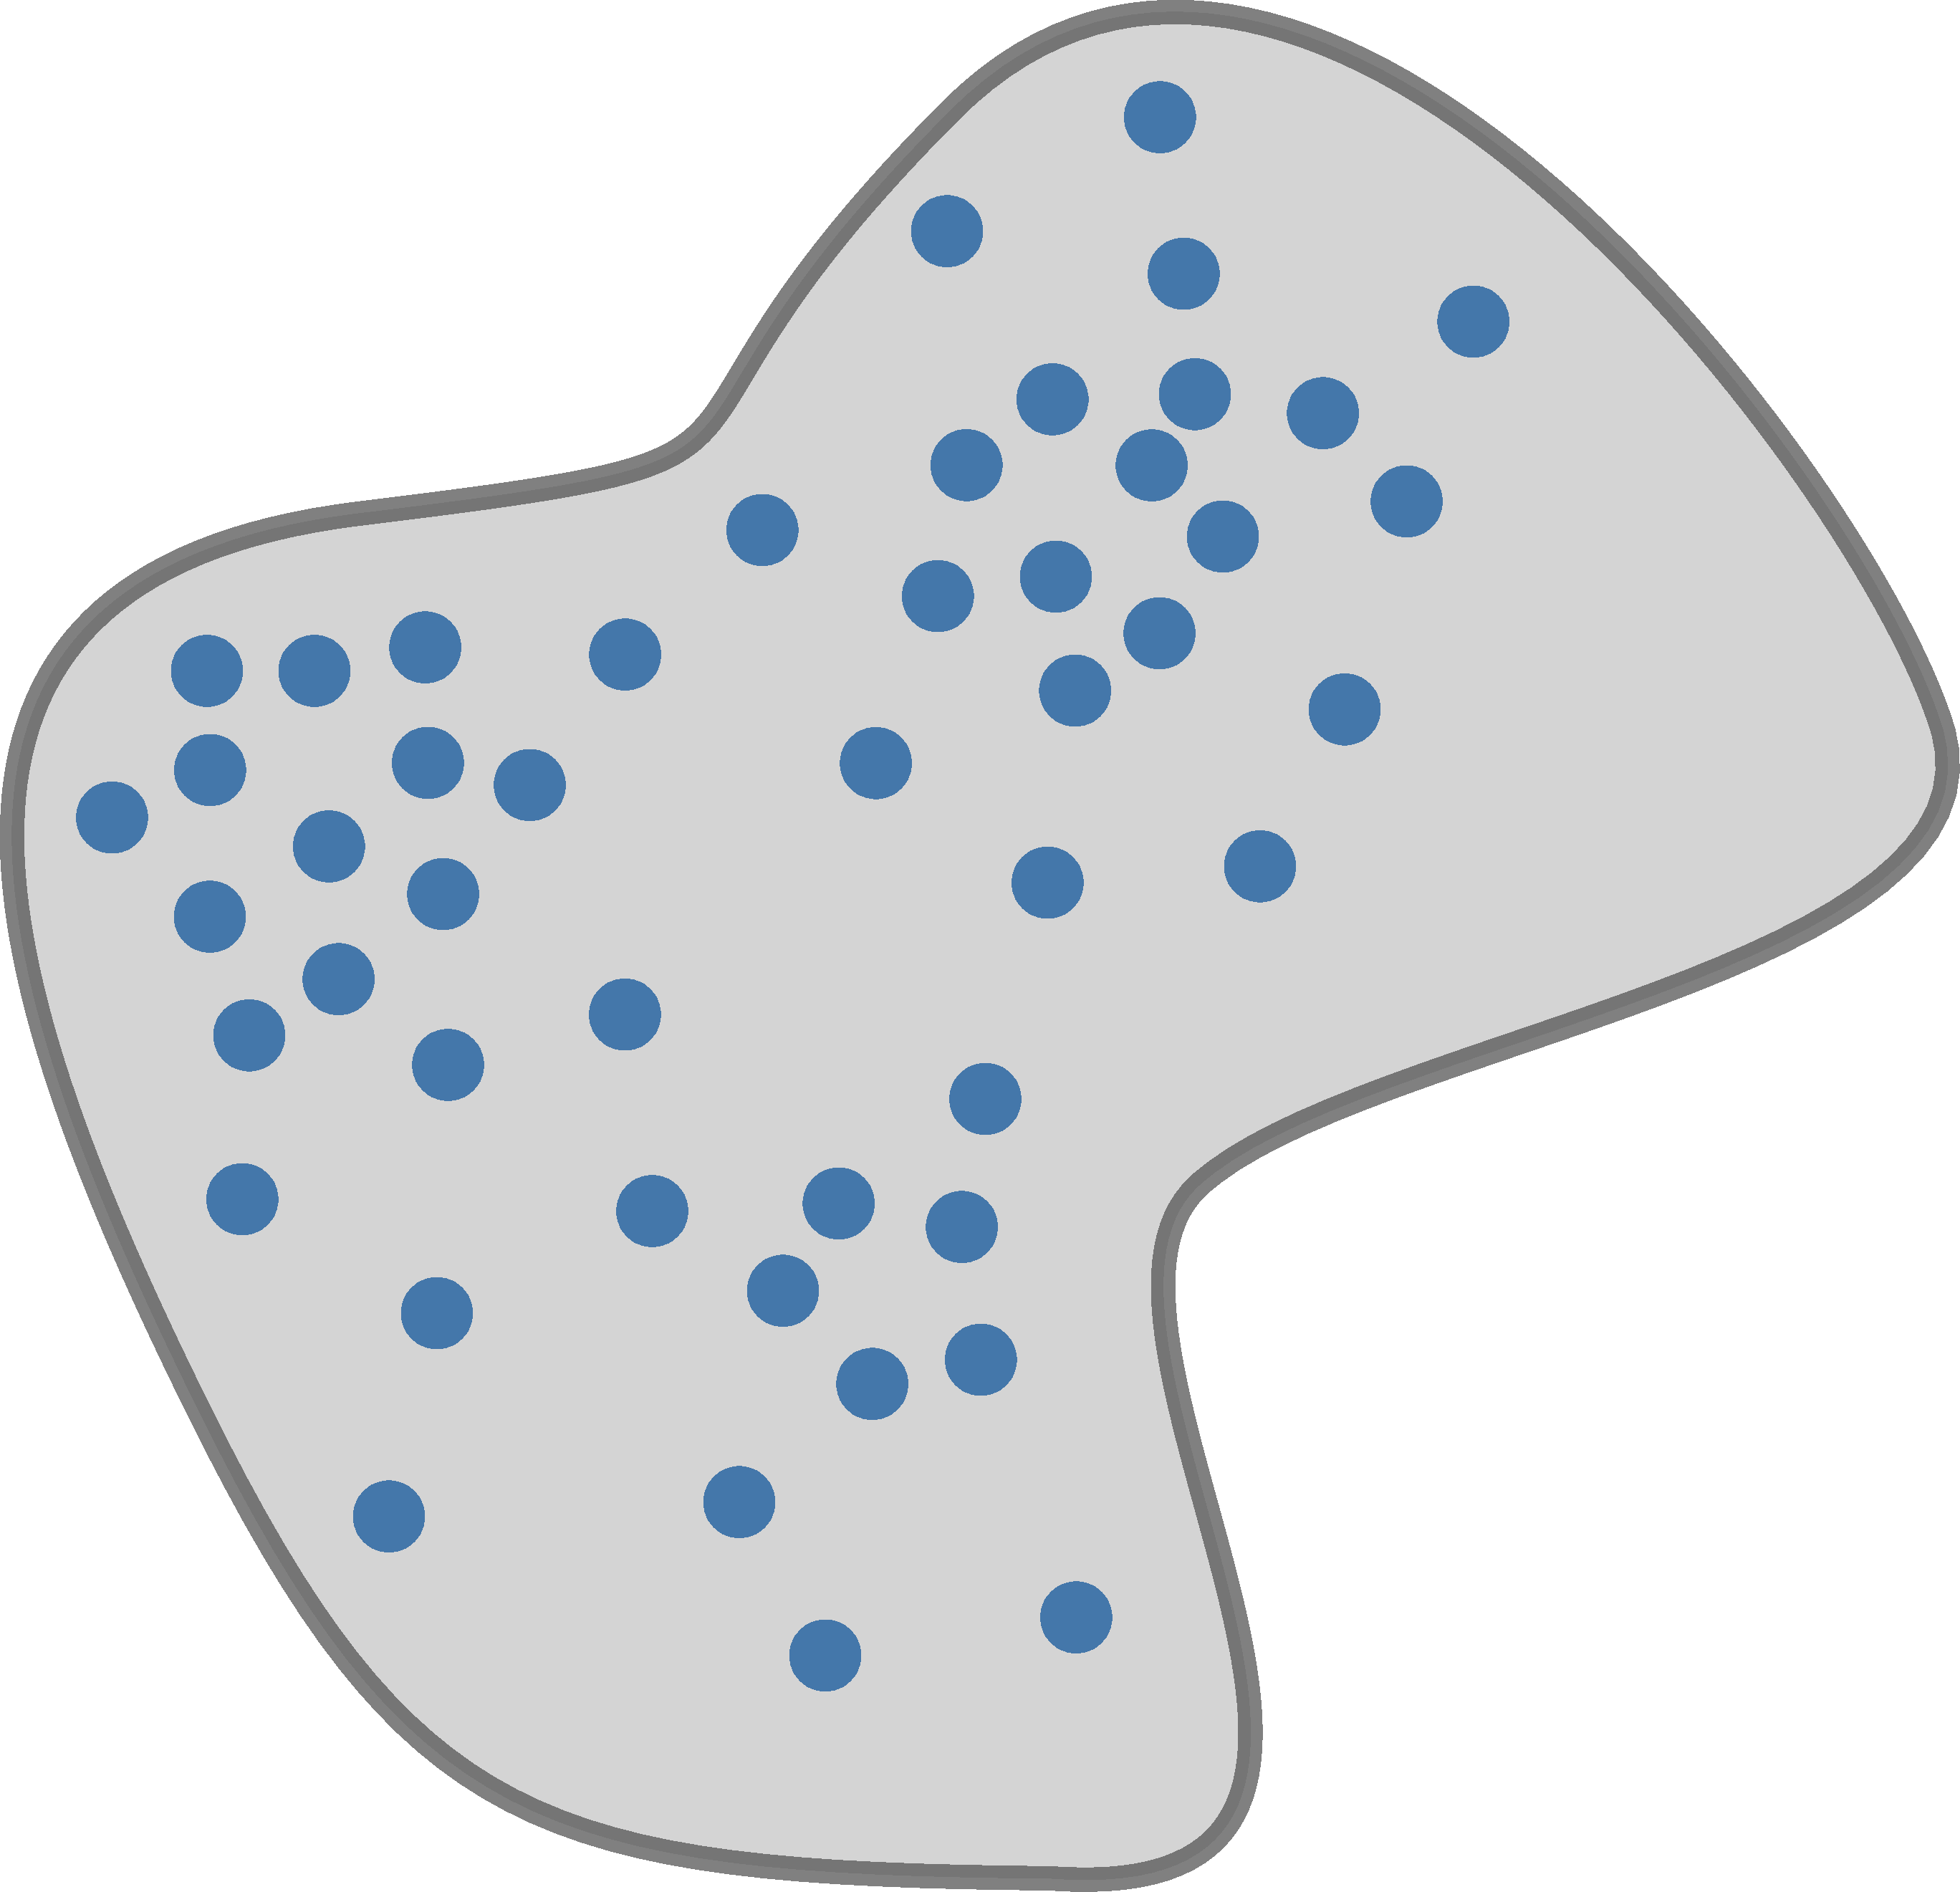
\includegraphics[align=t,height=7em]{images/volumeintegral.pdf}
\end{center}
we have eliminated one spatial dimension for simplicity, and considered the analogous two-dimensional idea. The region is in \textcolor{blue}{light blue}, delimited by a closed \textcolor{cyan} boundary. This is a snapshot at a given time instant. The number of points inside the boundary gives us an idea of the amount of matter that's within the region at this instant. Actually the points do more: they give us the idea that there's a higher amount of matter in some sub-regions, and lower amount in others. This is extra information that we don't need right now but will be useful later.

As a mental picture, this can be a good start. Let's straighten out some of its aspects.

The first aspect of the picture that we must be cautious about is the discreteness of the points. Sure, in some physical situations matter can be considered discrete; the points might represent atoms for instance. But in many common situations it's more advantageous to think of matter as being \emph{continuously distributed} within the region, even if it can be absent in some subregions, and if its \emph{density} may be higher or lower here or there. In this case the points in the picture only give us a qualitative indication of the density, they don't represent real discrete bunches of matter. Also, matter was here taken only as a concrete example; the quantity in question could be \emph{energy} instead, which is often continuously distributed.

The second aspect is that some of the quantity within the region might be positive, and some negative. This is commonly true for electric charge, and can be true for matter as well (antimatter). We could represent this by using \textcolor{red}{red} points for the subregions containing quantity of negative sign, like negative electric charge or antimatter:
\begin{center}
  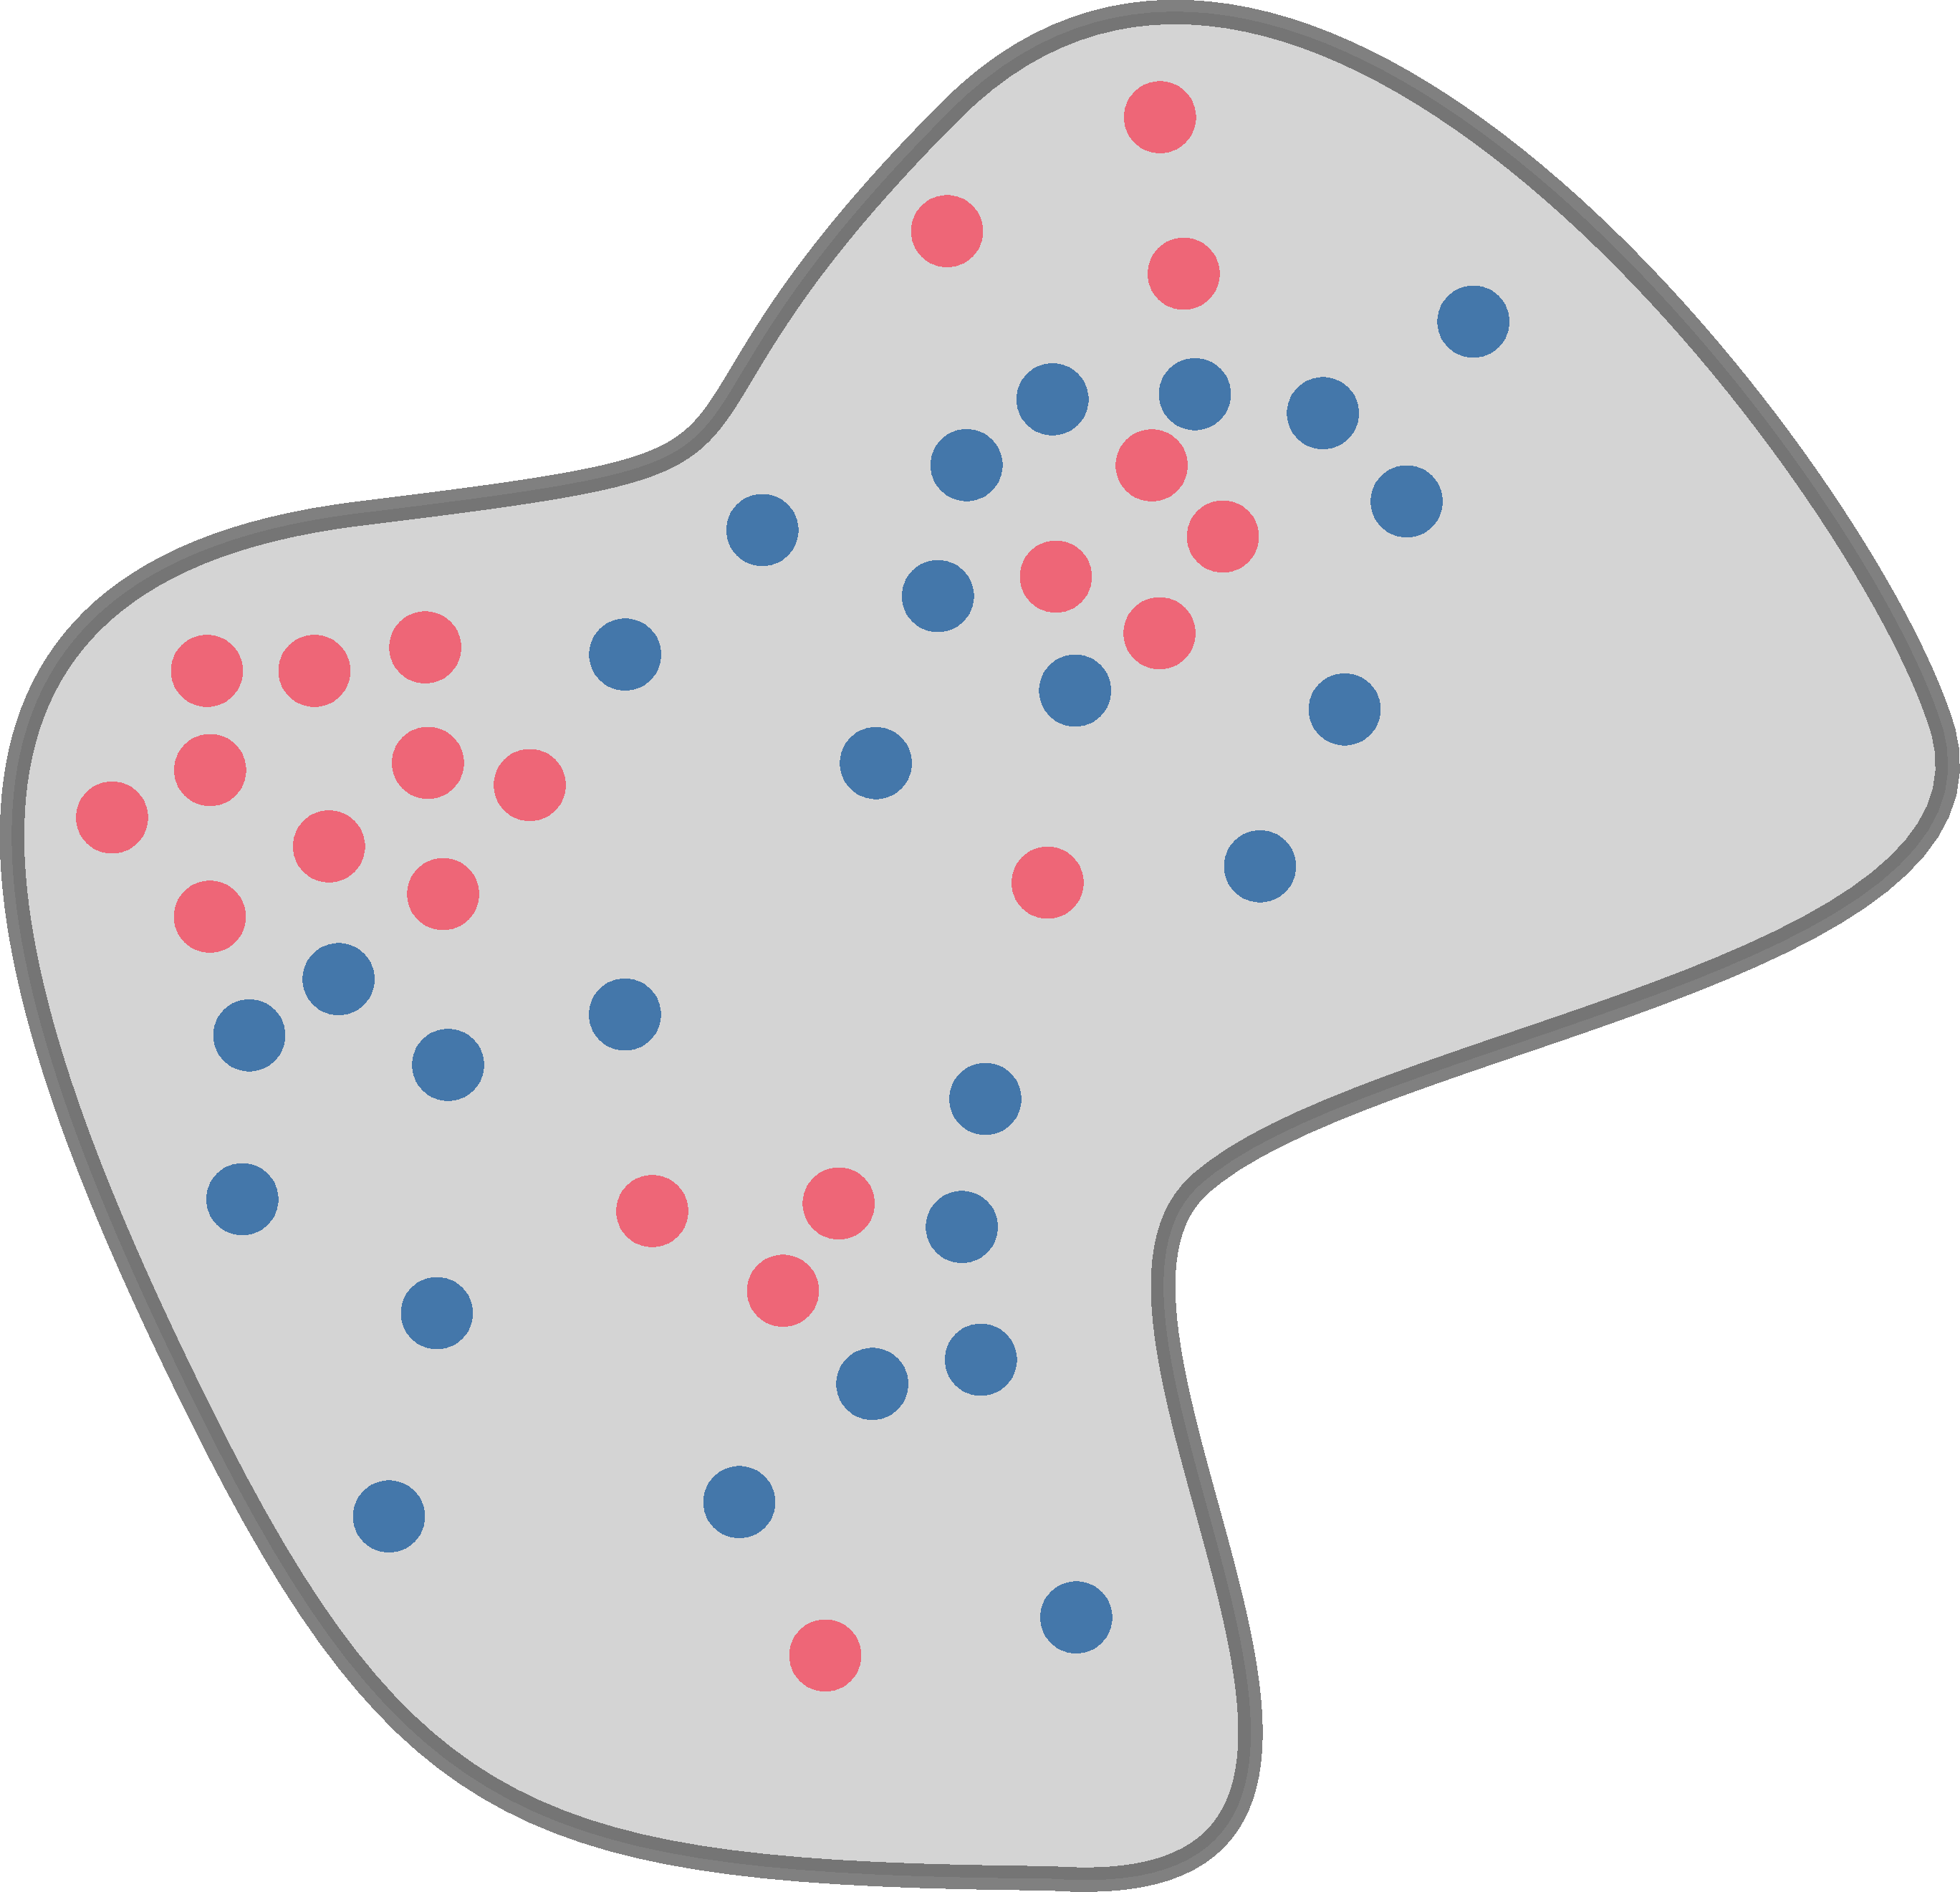
\includegraphics[align=t,height=7em]{images/volumeintegral_neg.pdf}
\end{center}
Now we realize something important: \emph{the total amount of a quantity in a region can be zero, and yet the amount in subregions can be non-zero.}

So if we measure the total amount of a quantity in a region and find a value of zero, we still don't know what are the amounts within different subregions: some of them could be positive and other negative; unless we have physical grounds to rule out this possibility, of course. This lack of information is \emph{not} necessarily a difficulty when solving physical problems. But you must take it into consideration when forming mental pictures of the situation, and make allowance for the various possibilities. For instance, imagine that there's a lot of positive and a lot of negative quantity in the region; what you know is the difference or discrepancy between the two.
\marginpar{\footnotesize%
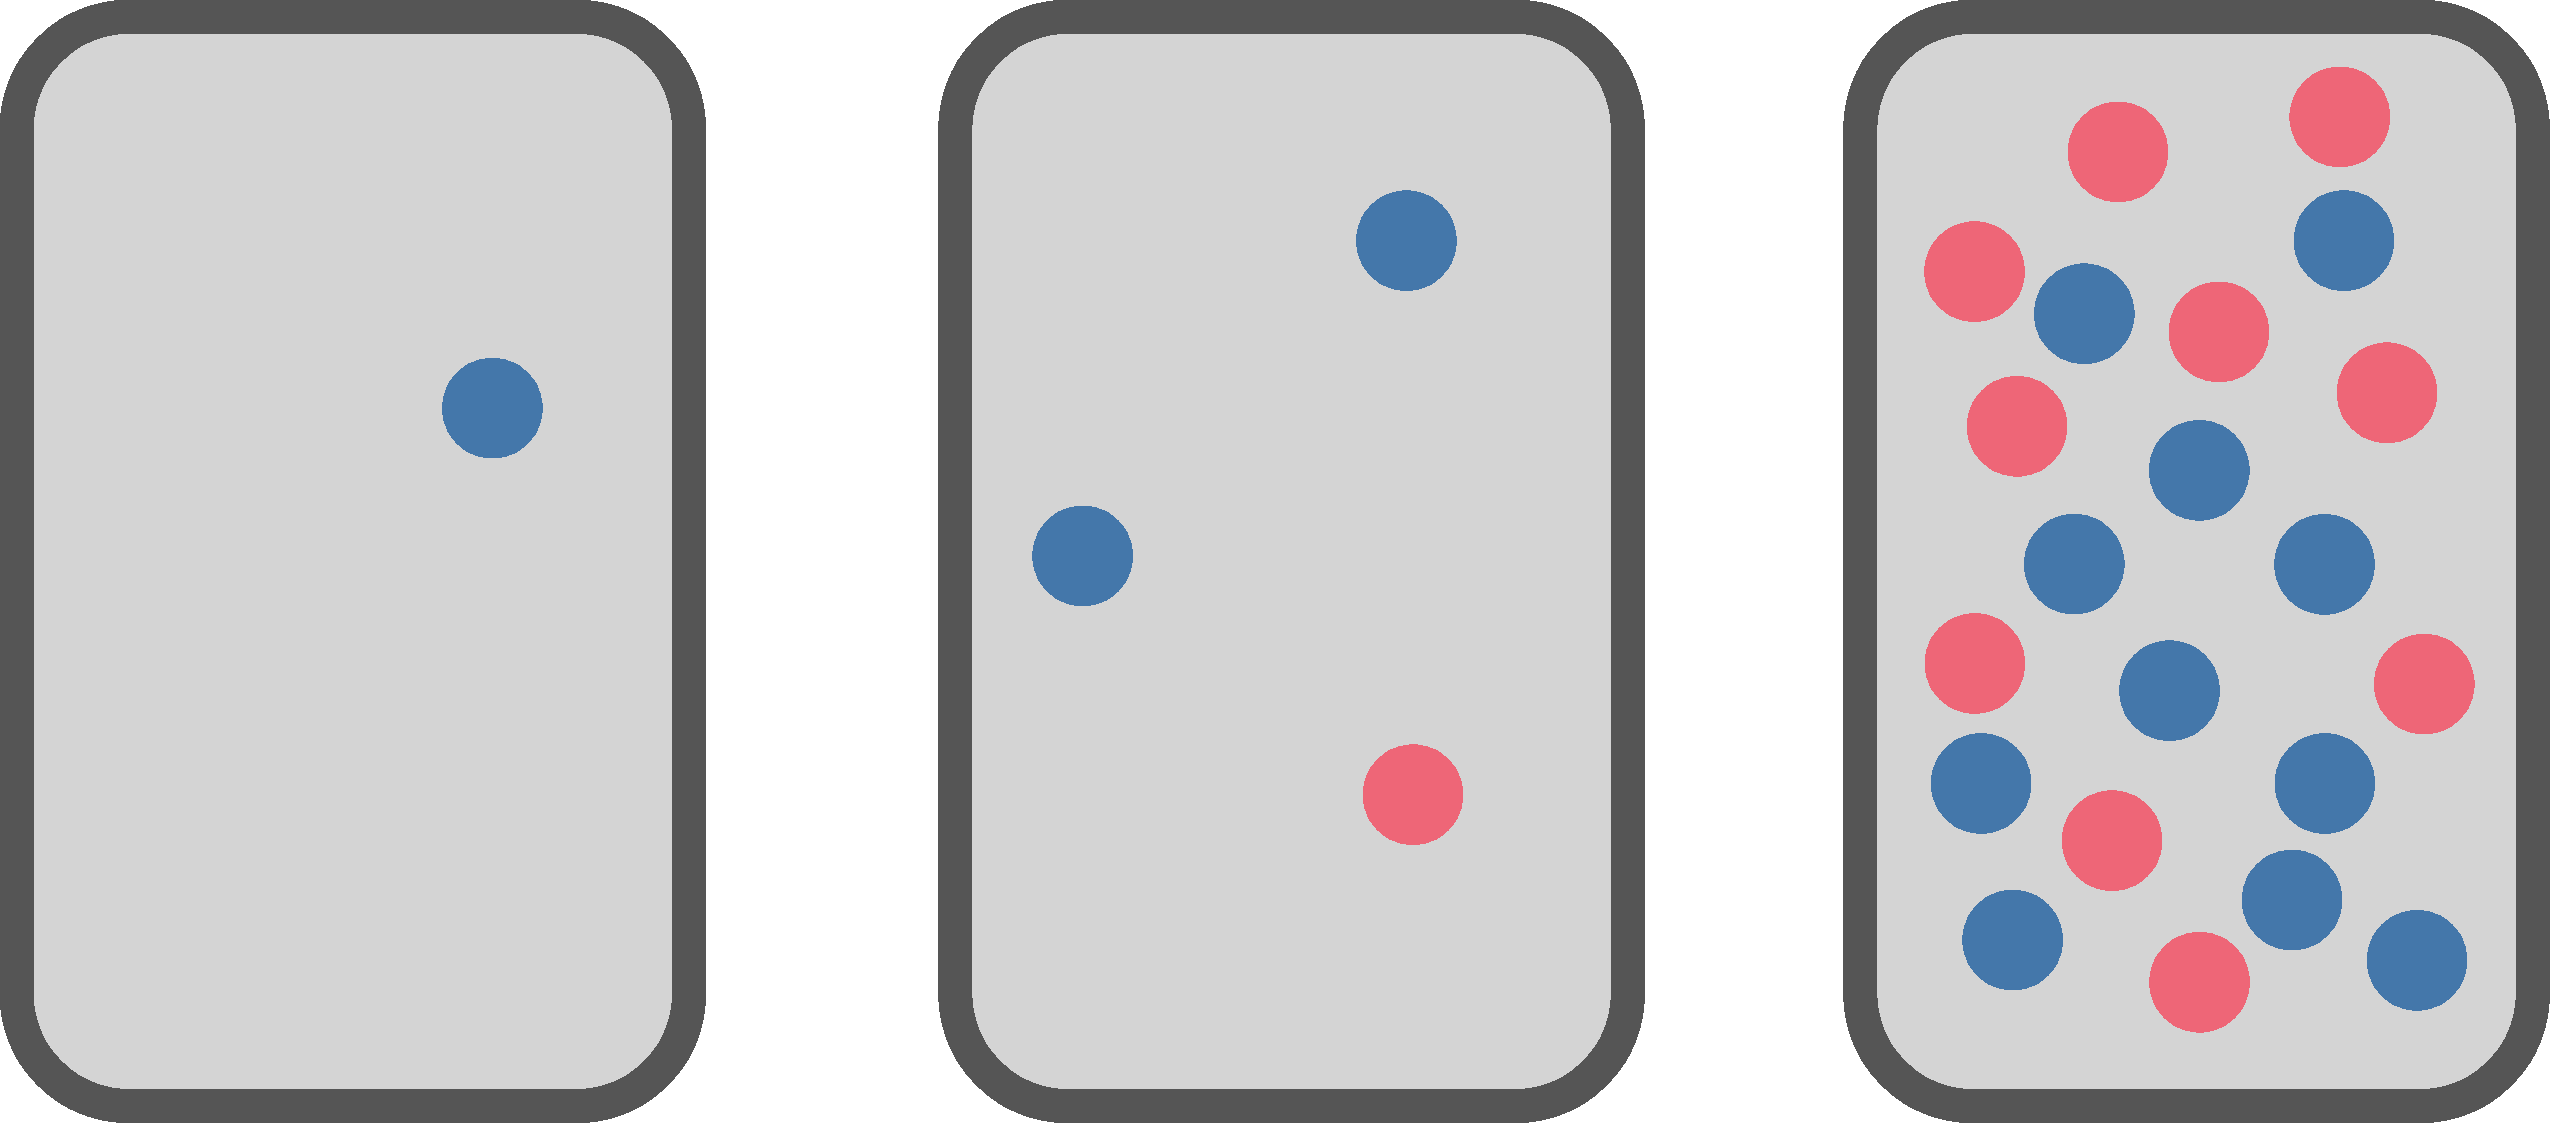
\includegraphics[align=t,width=\linewidth]{images/equivalent_VI.pdf}
% \\[\jot]%
% {\color{mpcolor}\enquote{\emph{%
% }}\sourceatright{\cites{}}}
}



The total is given by the sum of positive and negative amounts, and it could even be zero!


----



  , and we say that through this surface\noprelistbreak
\begin{center}%\color{green}
  there is a flux of momentum from the person to the wall,\\
  and the flux vector has a \textcolor{blue}{person$\rightarrow$wall orientation}
\end{center}

\noindent{this also mean that which, zooming in, can be depicted like this:\noprelistbreak
  \begin{center}
        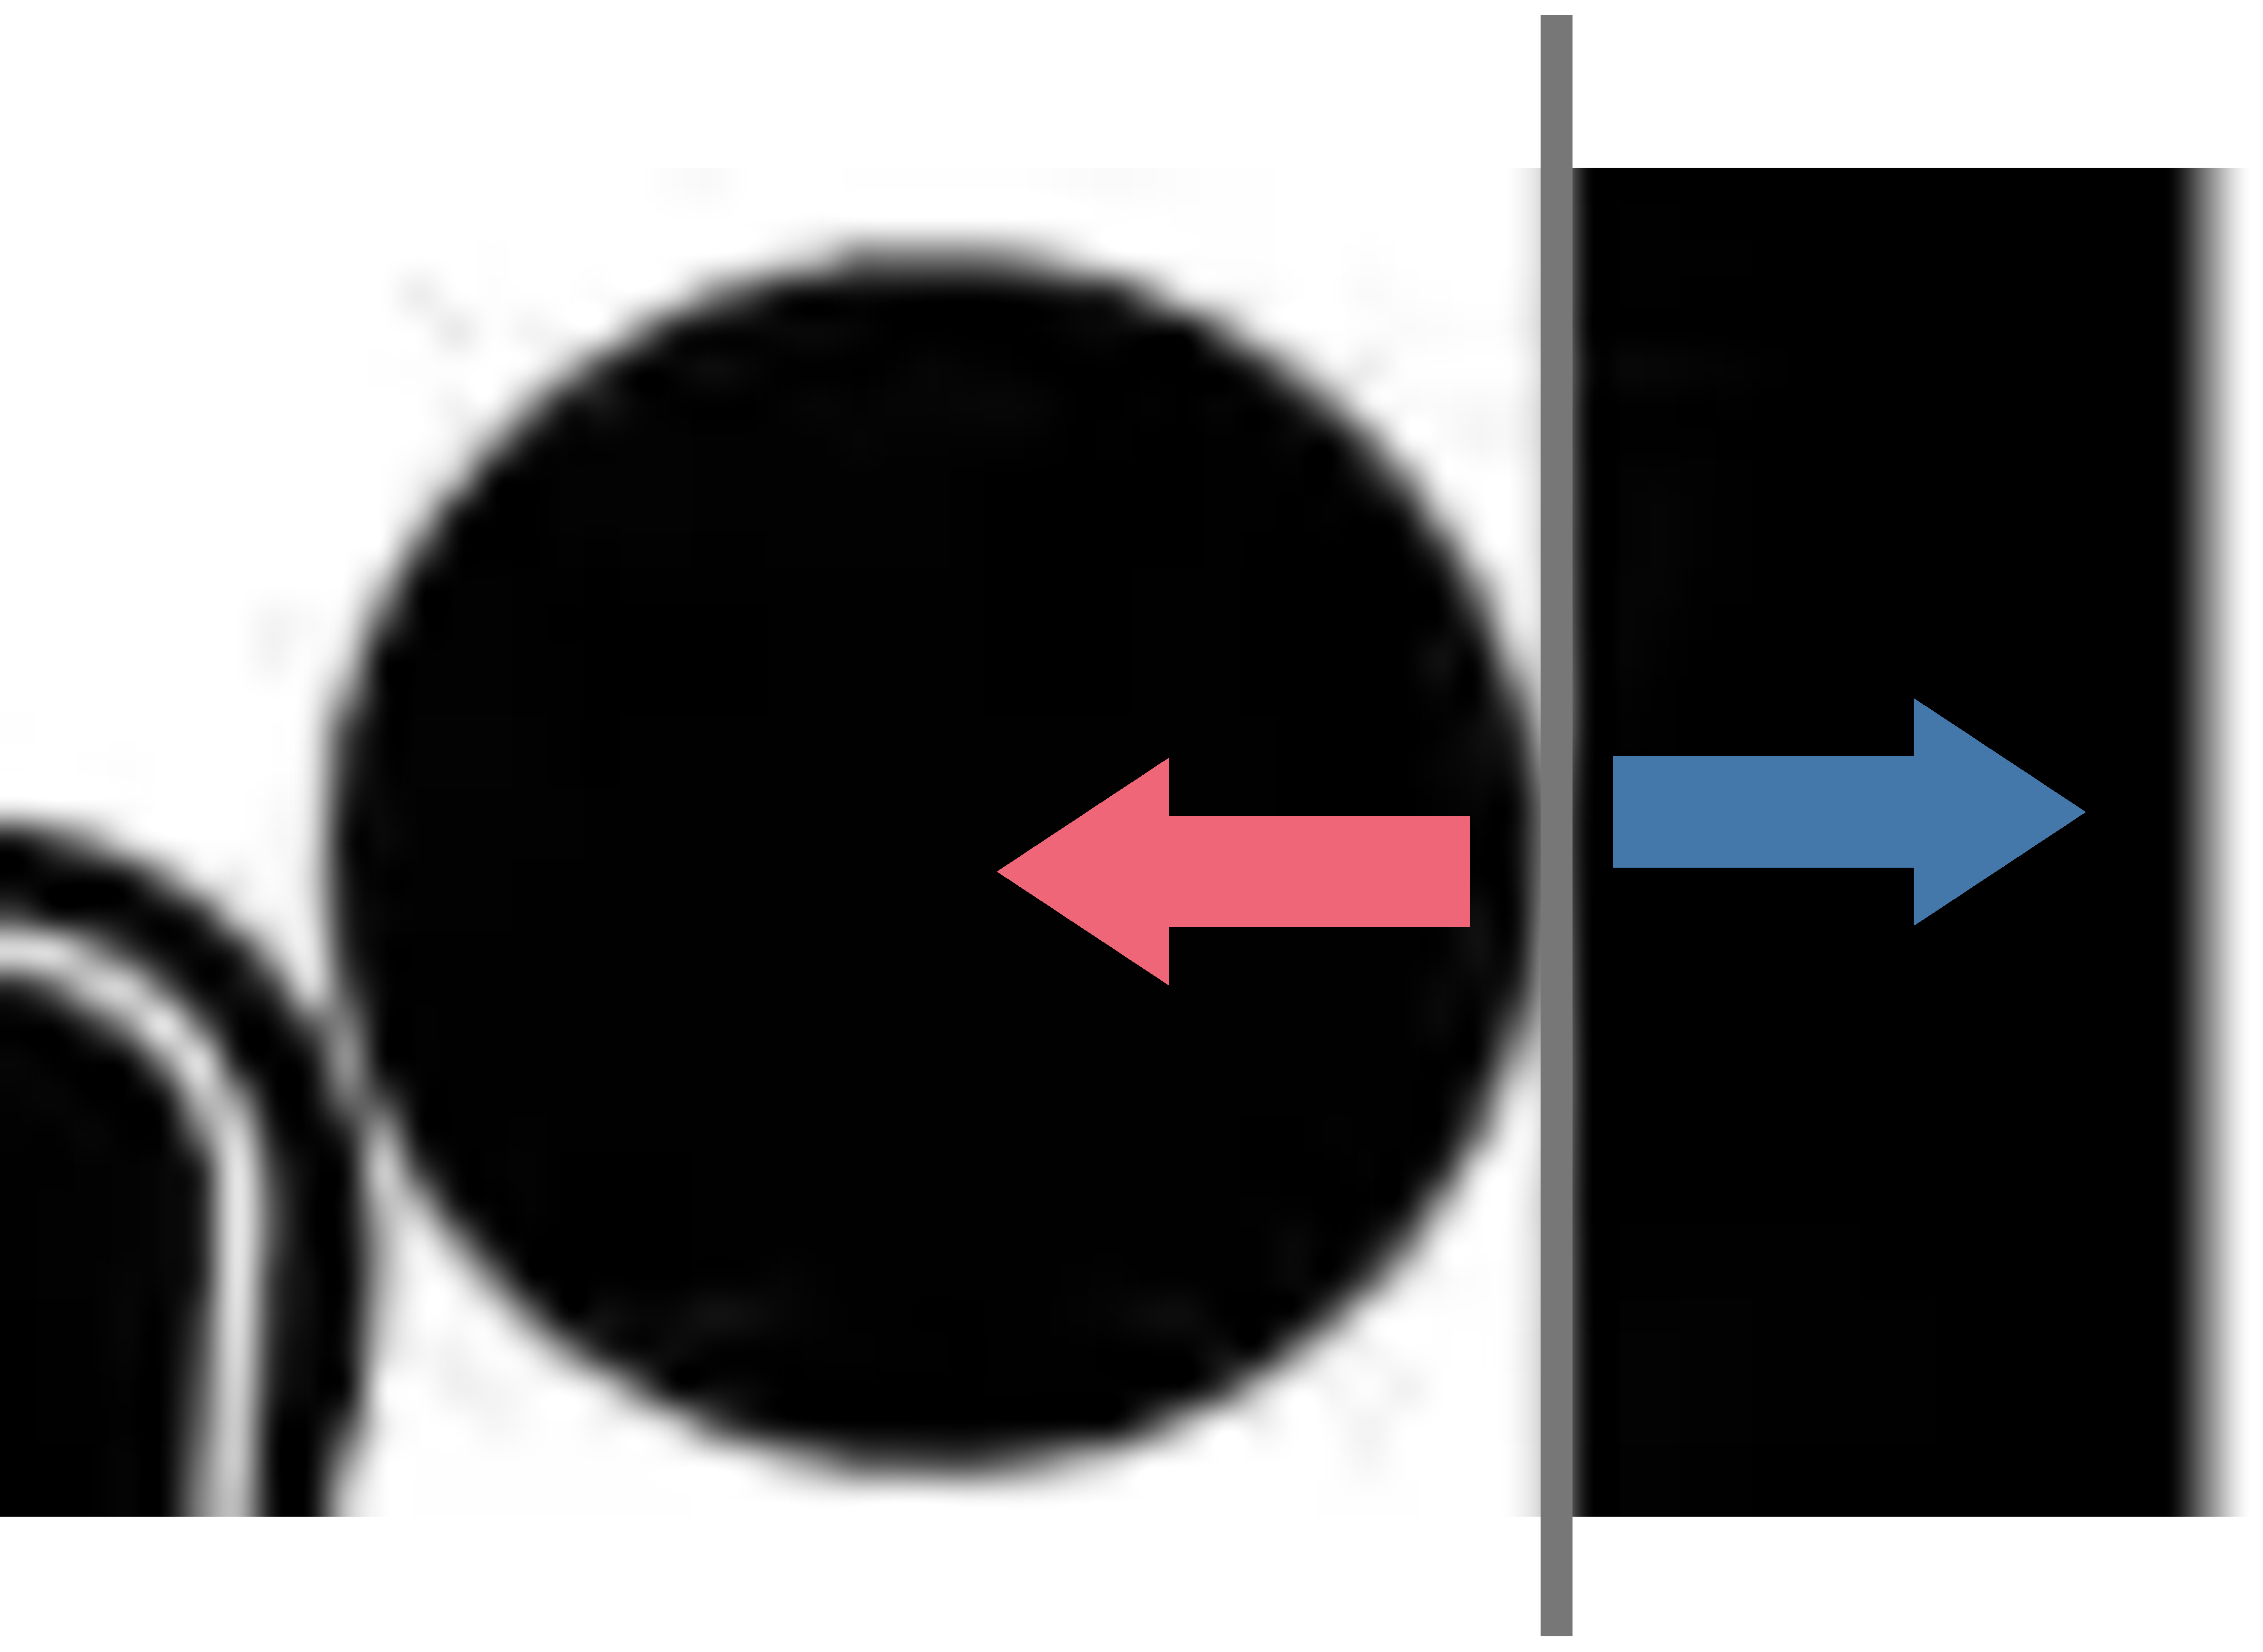
\includegraphics[width=1\marginparwidth]{images/person_push_flux.pdf}
  \end{center}
}

\bigskip

In the rest of these notes we shall use the terms \enquote*{momentum flux} and \enquote*{force} interchangeably, as synonymous words for the same thing. You can choose the mental representation that you prefer for this; but I recommend that you keep in mind the flux visualization. If a physics problem involving forces seems tricky, try to visualize them as momentum flow: suddenly the problem might become clearer.




% Suppose that at a given time instant we have this surface:
% \begin{center}
%   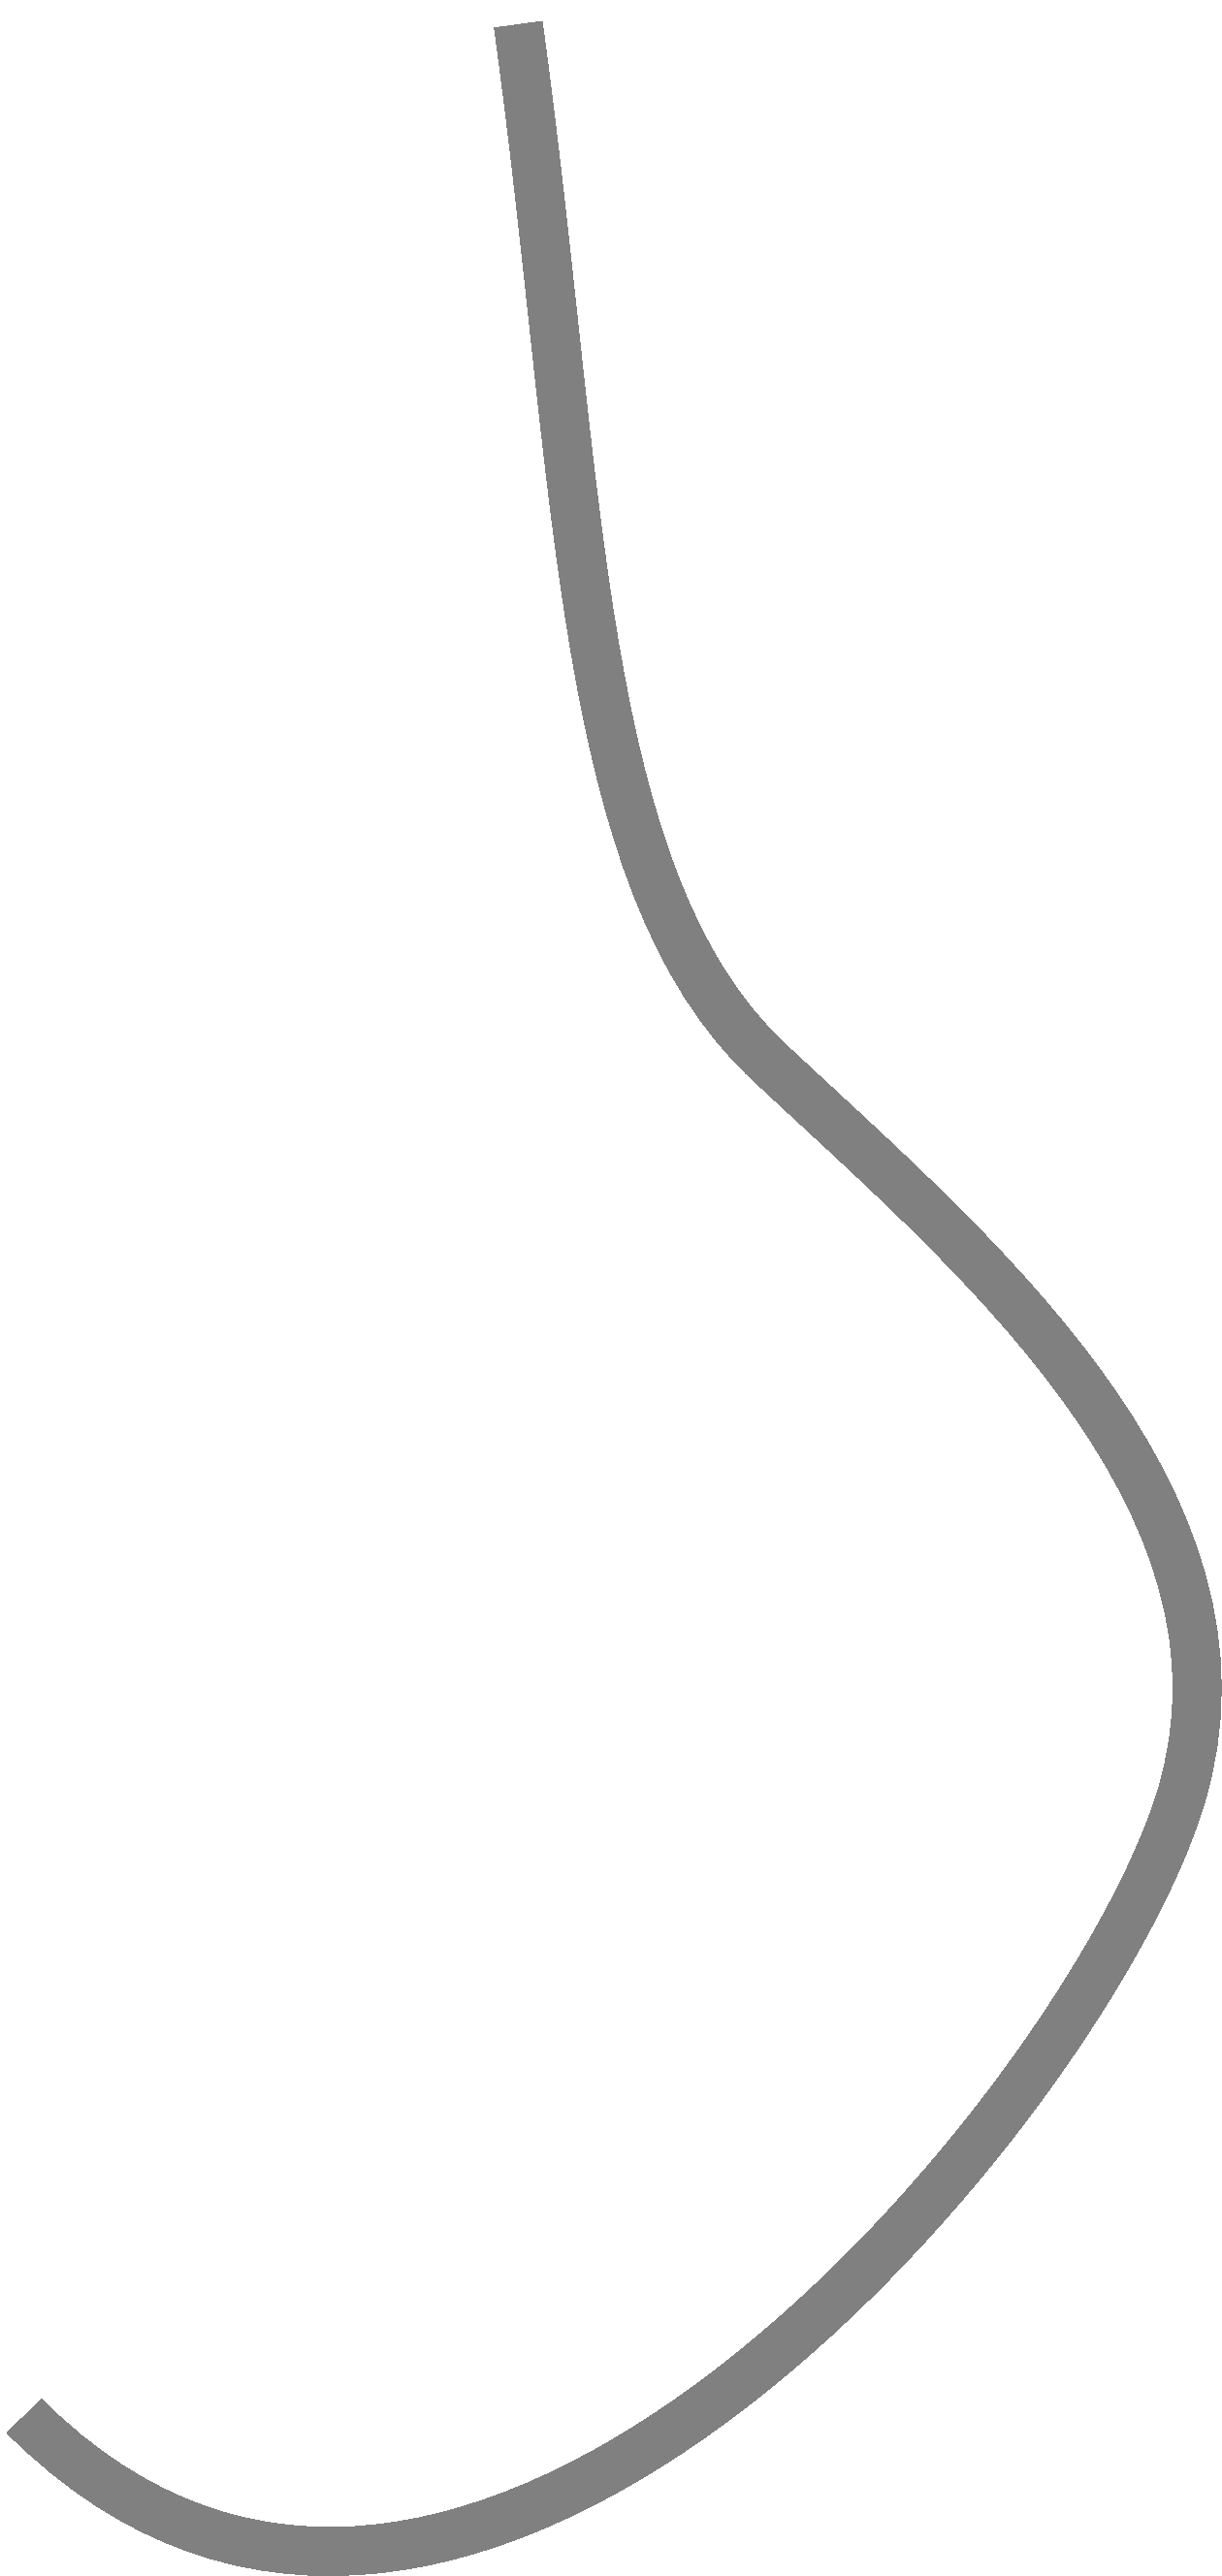
\includegraphics[height=7em]{images/fluxsurface.pdf}
% \end{center}
% where we have again eliminated one spatial dimension for simplicity. We want to visualize and graphically represent the fact that there's a flux of \textcolor{blue}{\qty{8}{J/s}} across this surface, from its left side to its right side.
%
% One first visualization that comes to mind is this:
% \begin{center}
%   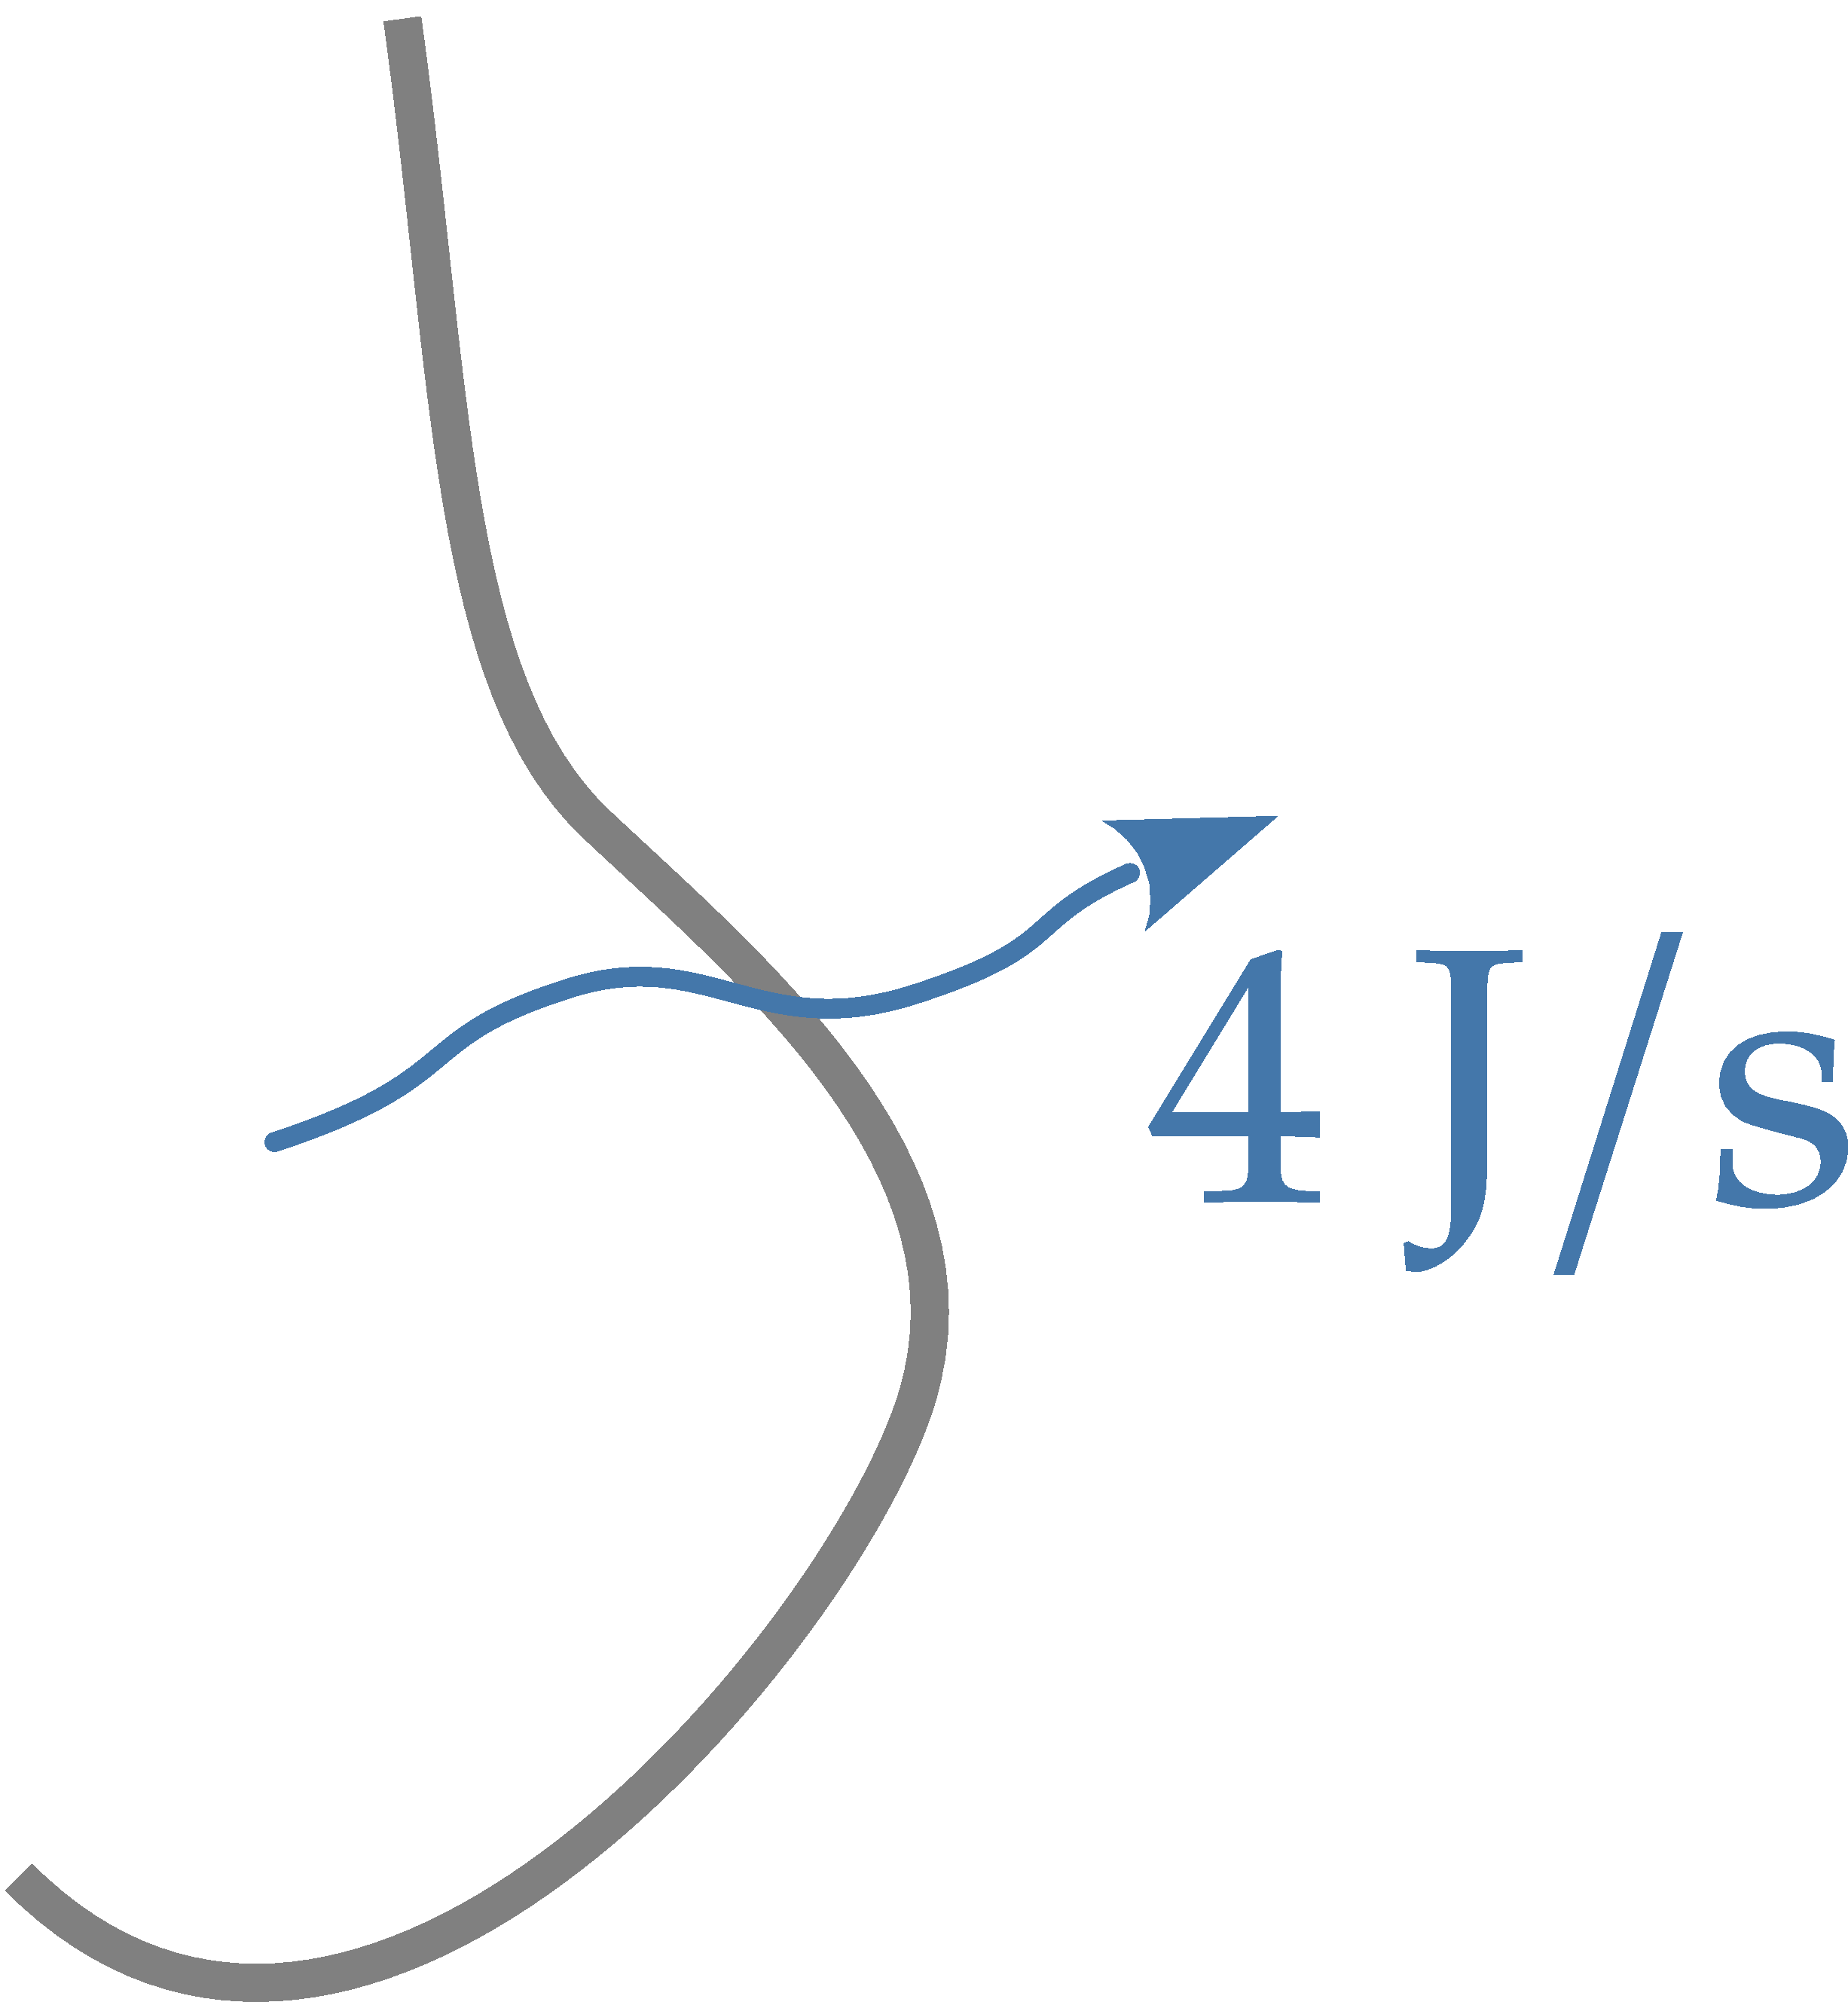
\includegraphics[align=c,height=7em]{images/flux_2J.pdf}
% \end{center}
% It conveys the correct information, but it's also misleading in several respects:
% \begin{itemize}[para]
% \item This is a snapshot at a given time instant. An instant earlier or later, the surface might be at a different position and with a different shape. The \textcolor{blue}{blue wiggly arrow} might suggest that the surface is at rest, while something crosses it.
%
% \item A flux, properly speaking,
% \marginpar{\footnotesize%
%   {\color{mpcolor}\enquote{\emph{%
% Fechner [in 1845] supposed every current to consist in a streaming of electric charges, the vitreous charges travelling in one direction, and the resinous charges, equal to them in magnitude and number, travelling in the opposite direction with equal velocity.}}\sourceatright{\cites{whittaker1910_r1951}}}
% }
% says that after a very small time interval there's a lower amount of a quantity on one side of a surface, and a larger amount on the other. \emph{But it doesn't say anything about a \enquote{left-to-right movement} of the quantity, or a right-to-left one}. In our example it could be that \textcolor{purple}{\qty{-4}{J/s}} of energy \enquote{moved} from right to left; or even that \qty{+7}{J/s} moved from left to right, and \qty{-3}{J/s} from right to left, possibly across different parts of the surface. All these possibilities correspond to the same flux. Moreover, \emph{the description of this situation depends on the coordinate system}: in one coordinate system the surface may be at rest, but in another it may be moving.
% \end{itemize}
%
% Therefore we see that the flux of our example could be happening in several ways. Four equivalent ways are illustrated in \fig~\ref{nfig:flux_interpretation}; combination of those are also possible.
% \begin{figure}[h]\centering
% \begin{tabularx}{\linewidth}{|X|X|X|X|}
% \centering  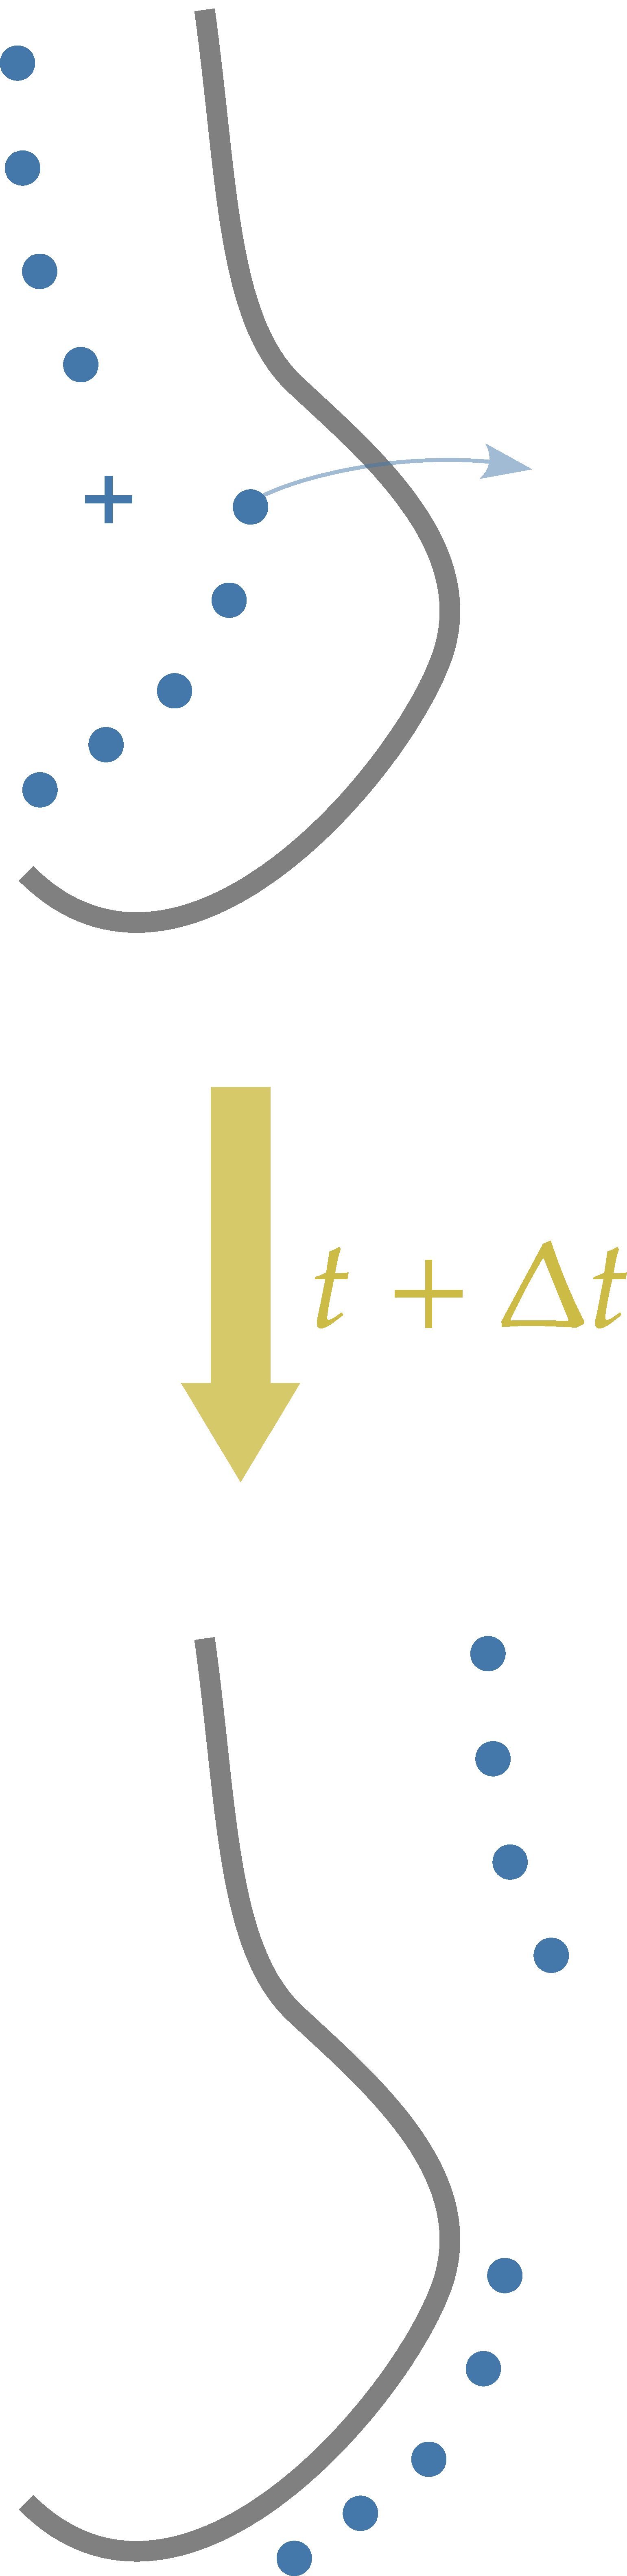
\includegraphics[align=t,height=21em]{images/flux_pq.pdf}
% &
% \centering   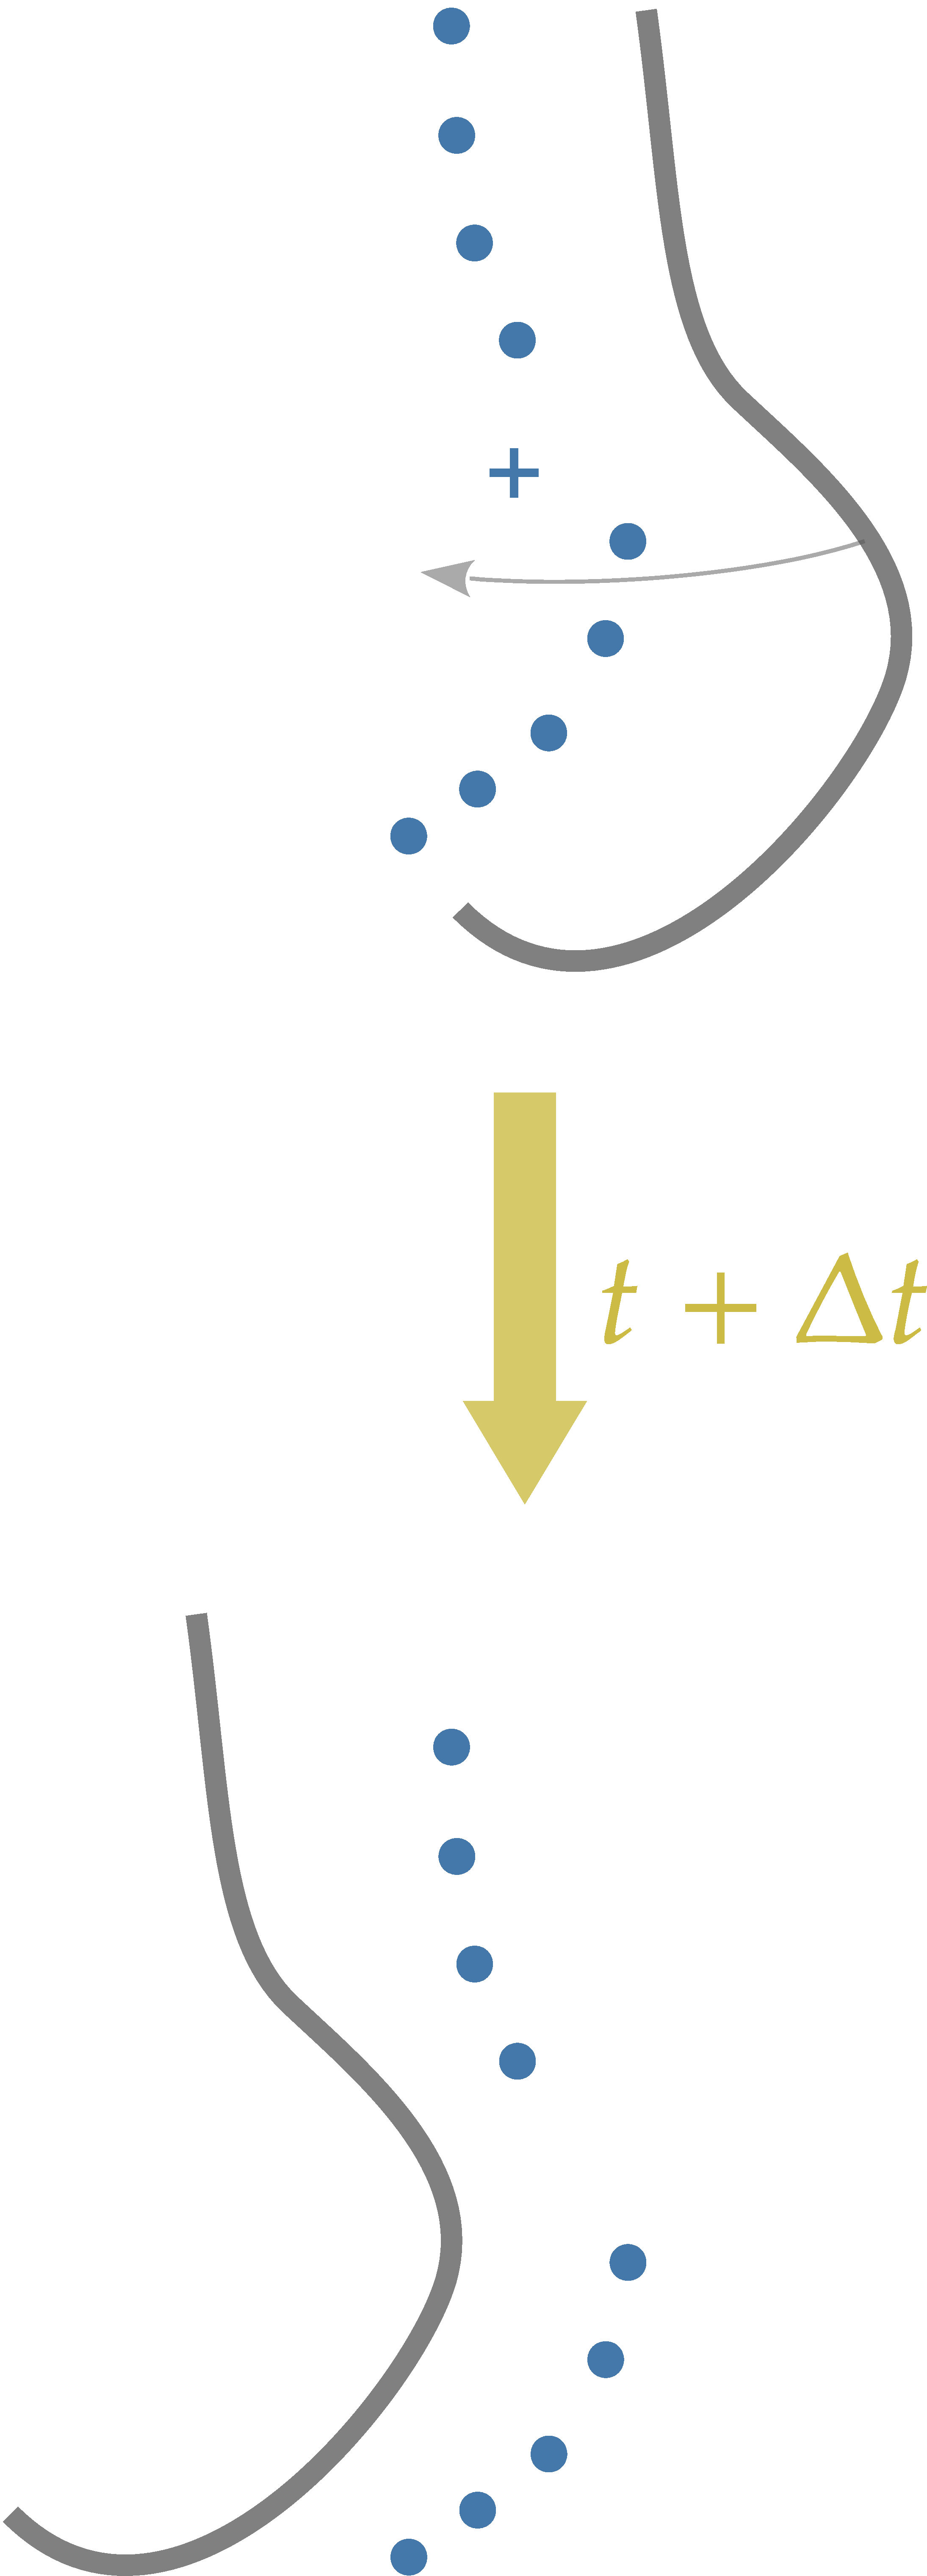
\includegraphics[align=t,height=21em]{images/flux_ps.pdf}
% &
% \centering   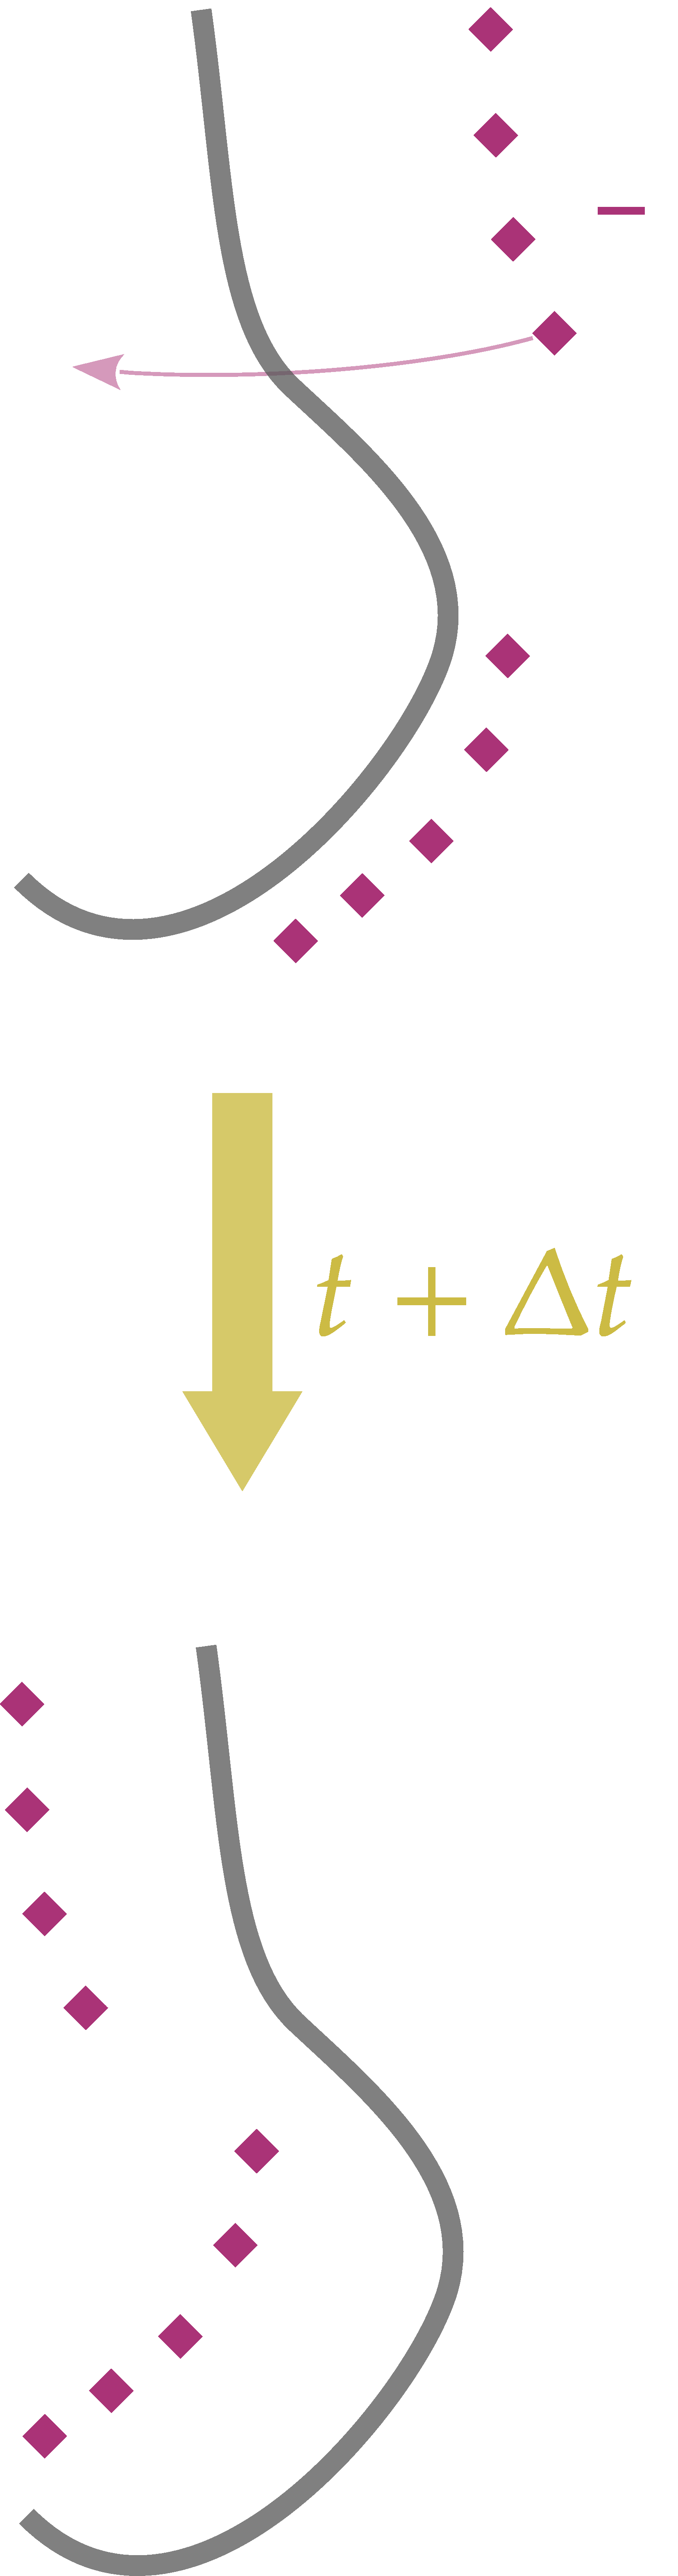
\includegraphics[align=t,height=21em]{images/flux_mq.pdf}
% &
% \centering   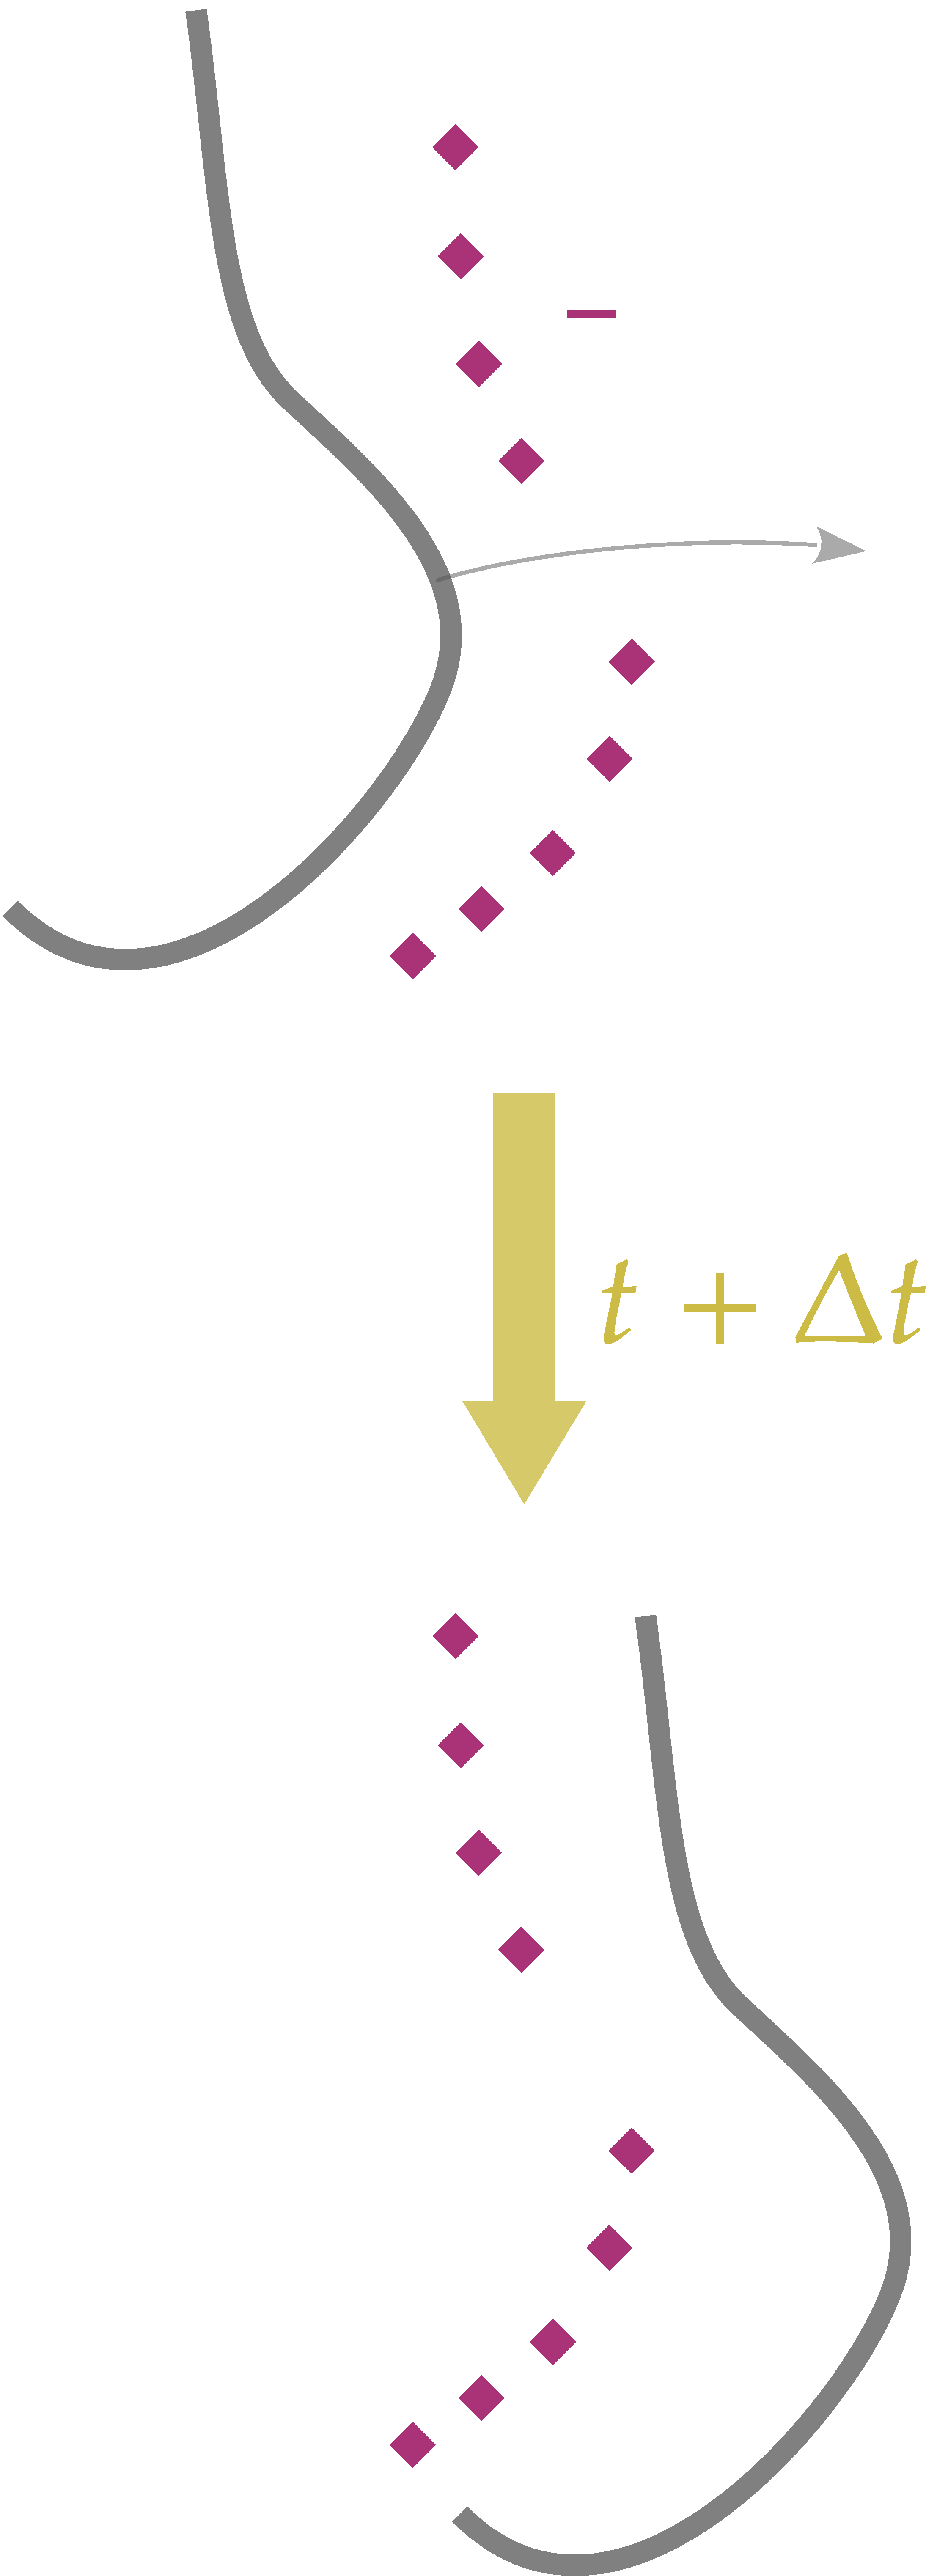
\includegraphics[align=t,height=21em]{images/flux_ms.pdf}
%   \end{tabularx}
%   \caption{Four allusive depictions of the same flux}\label{nfig:flux_interpretation}
% \end{figure}
%
% \medskip
%
% \begin{samepage}
%   In view of these possibilities, a less misleading representation of the flux in our example could be as follows:
%   \begin{center}
%     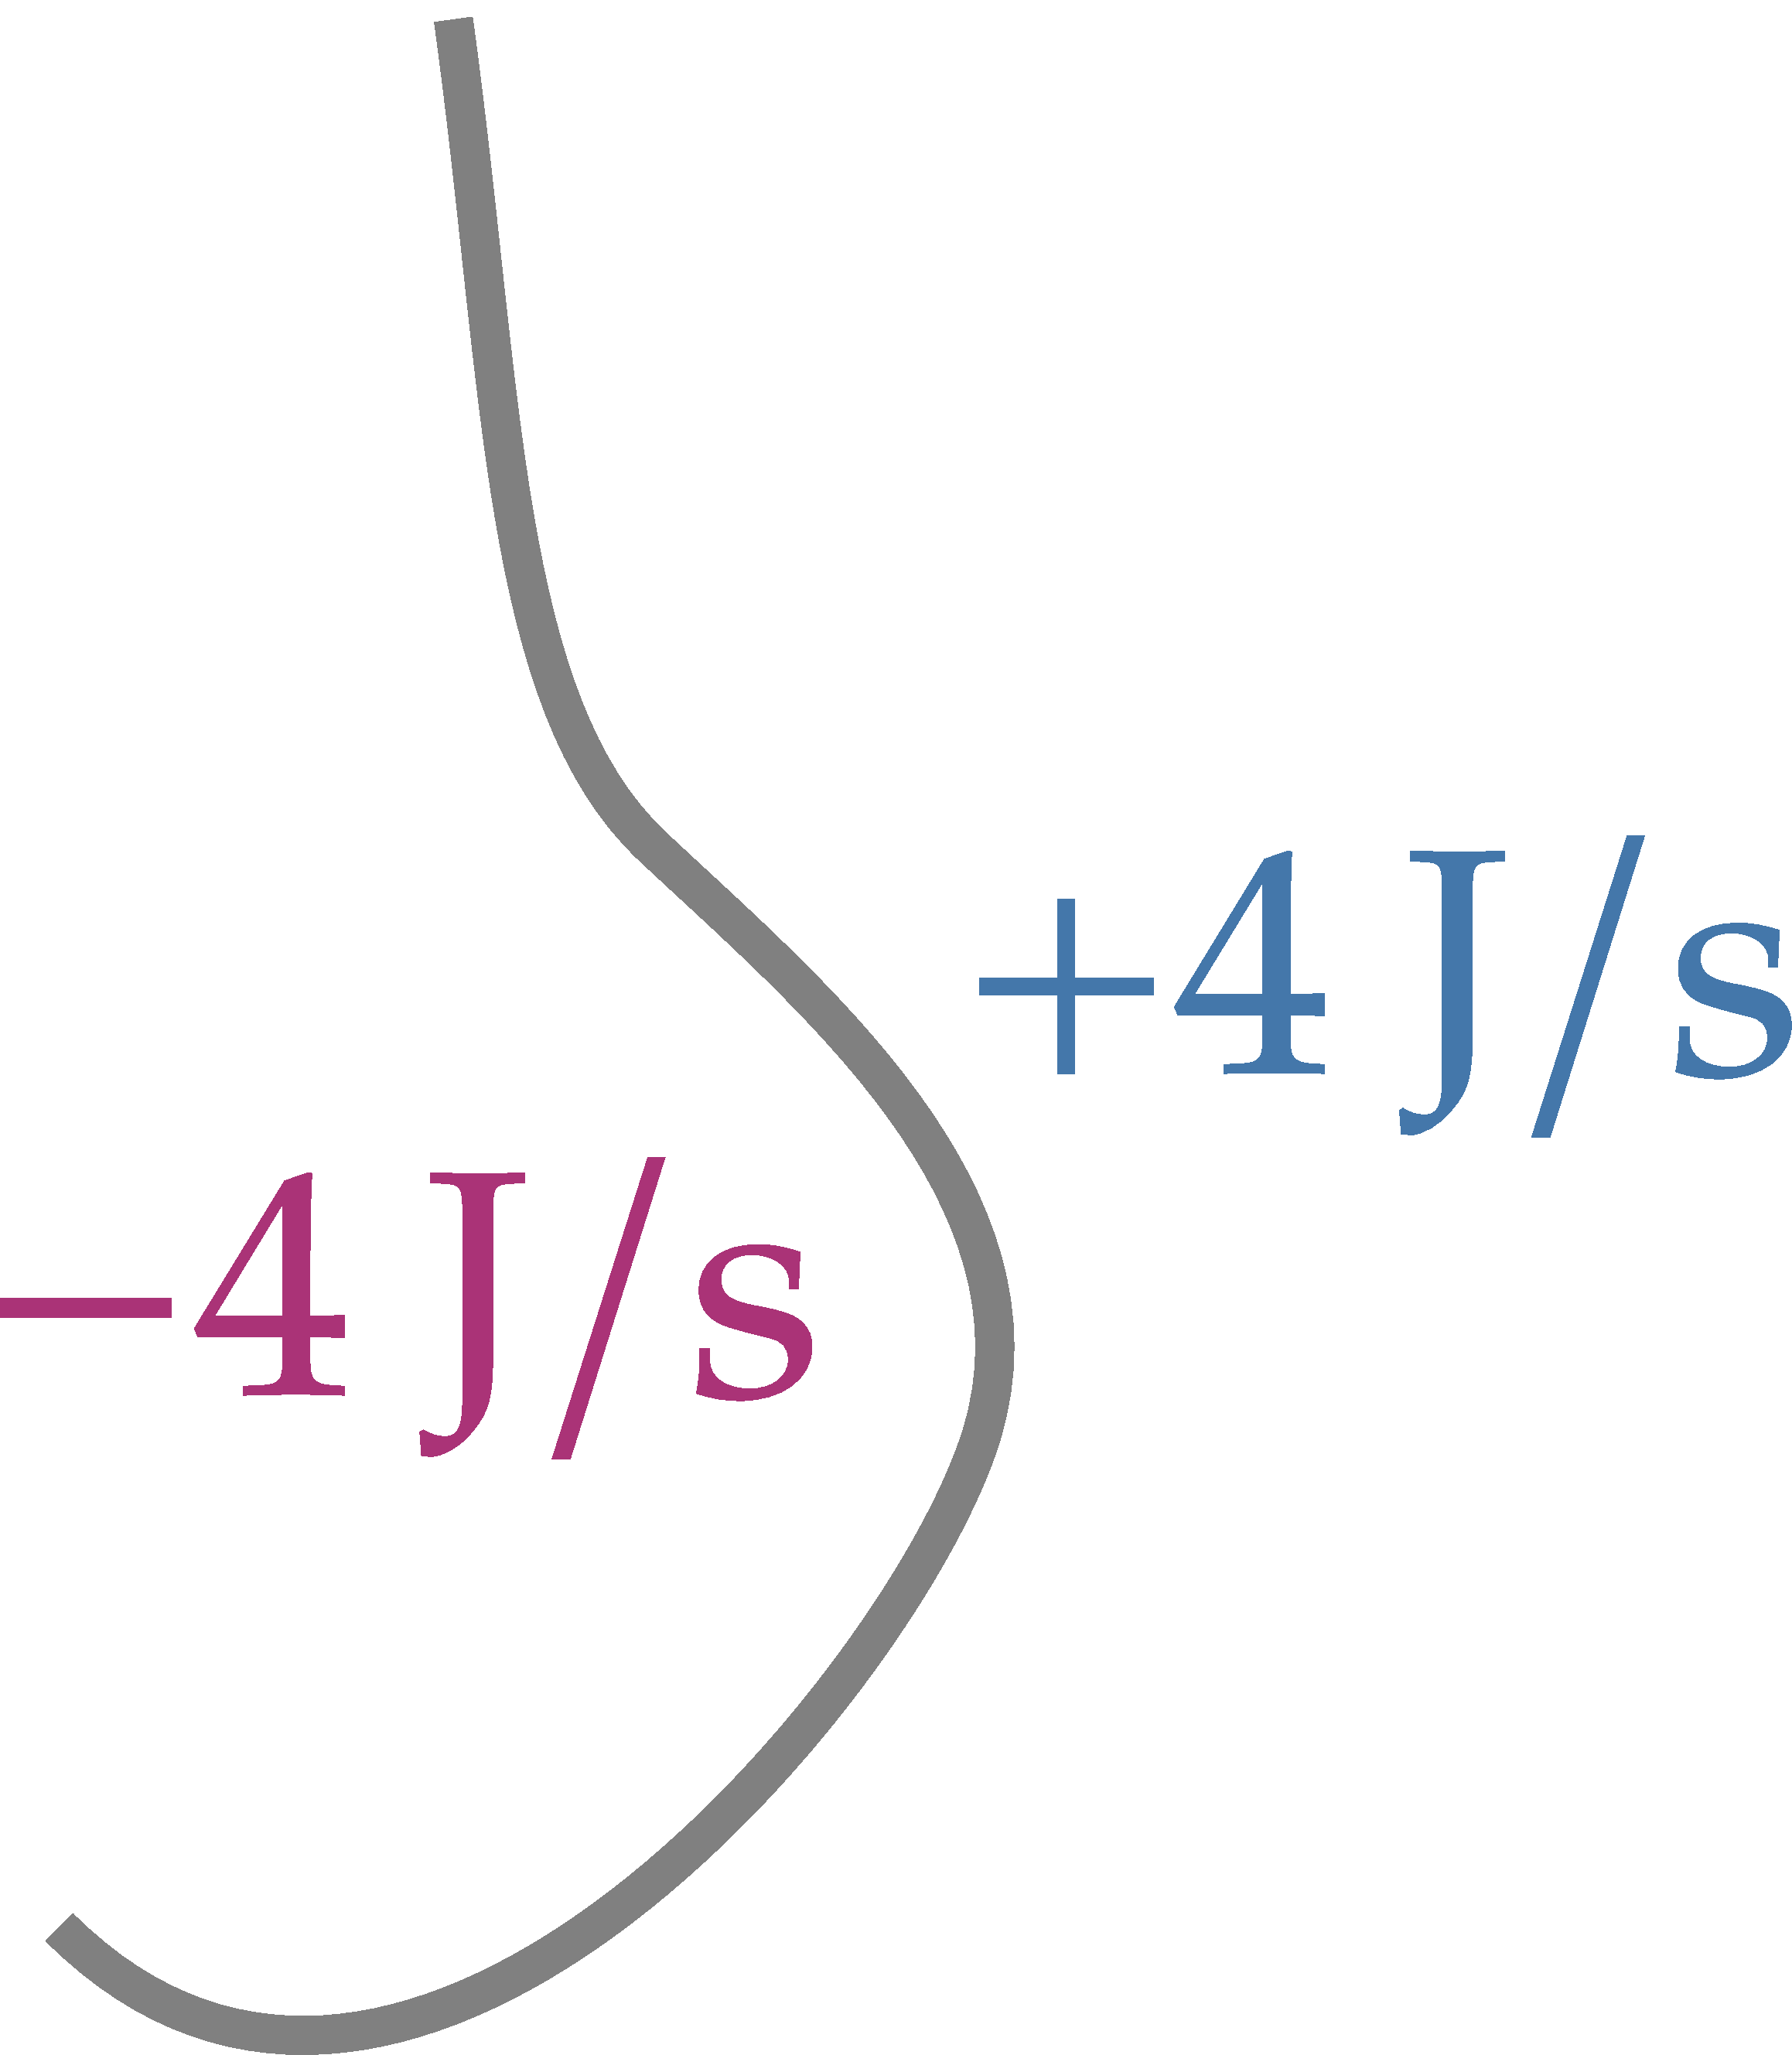
\includegraphics[height=7em]{images/flux_both.pdf}
%   \end{center}
% \end{samepage}
% This picture says that there's an energy change of \qty{-4}{J/s} on the left side of the surface, and of \qty{+4}{J/s} on the right. Note that \textbf{the amounts indicated on the two sides must have equal magnitude but opposite sign}, otherwise the picture doesn't make sense. The absence of arrows prevents unwarranted conclusions about \enquote{what's moving}. If we know that the surface is moving in a particular way, then arrows could of course be added to indicate this movement.
%
% \smallskip
%
% Please feel free to use the graphical representation and mental visualization that you prefer. The ones above are just suggestions. The real goal of the discussion above was to make you are aware of the subtleties regarding flux, so that you don't make wrong assumptions and jump to wrong conclusions when solving physics problems.
%
% \bigskip
%
% % Our discussion shows an important mathematical and physical symmetry of the flux of a scalar quantity:
% % \begin{definition}{Every flux is the same as the opposite flux in the opposite direction}
% %   A flux of a given sign in a particular surface-crossing direction is equivalent to a flux of opposite sign in the opposite crossing direction.
% % \end{definition}
% %
% \begin{exercise}
%   The volume content of matter in a particular volume is equal to \qty{36}{mol}. Can we conclude that the volume doesn't contain antimatter?
% \end{exercise}


% add extra about quantum field theory \mynotew{}


\nonosection{Intuition and visualization for vector quantities}
\label{nsec:intuition_vector}

Let's now consider the vector quantities momentum and angular momentum.

\nonosubsection{Volume contents}



\bigskip

\nonosubsection{Fluxes}

For the visualization and mental representation of the flux of a vector quantity we must pay attention to analogous warnings as for a scalar quantity. Consider again our example surface
\begin{center}
  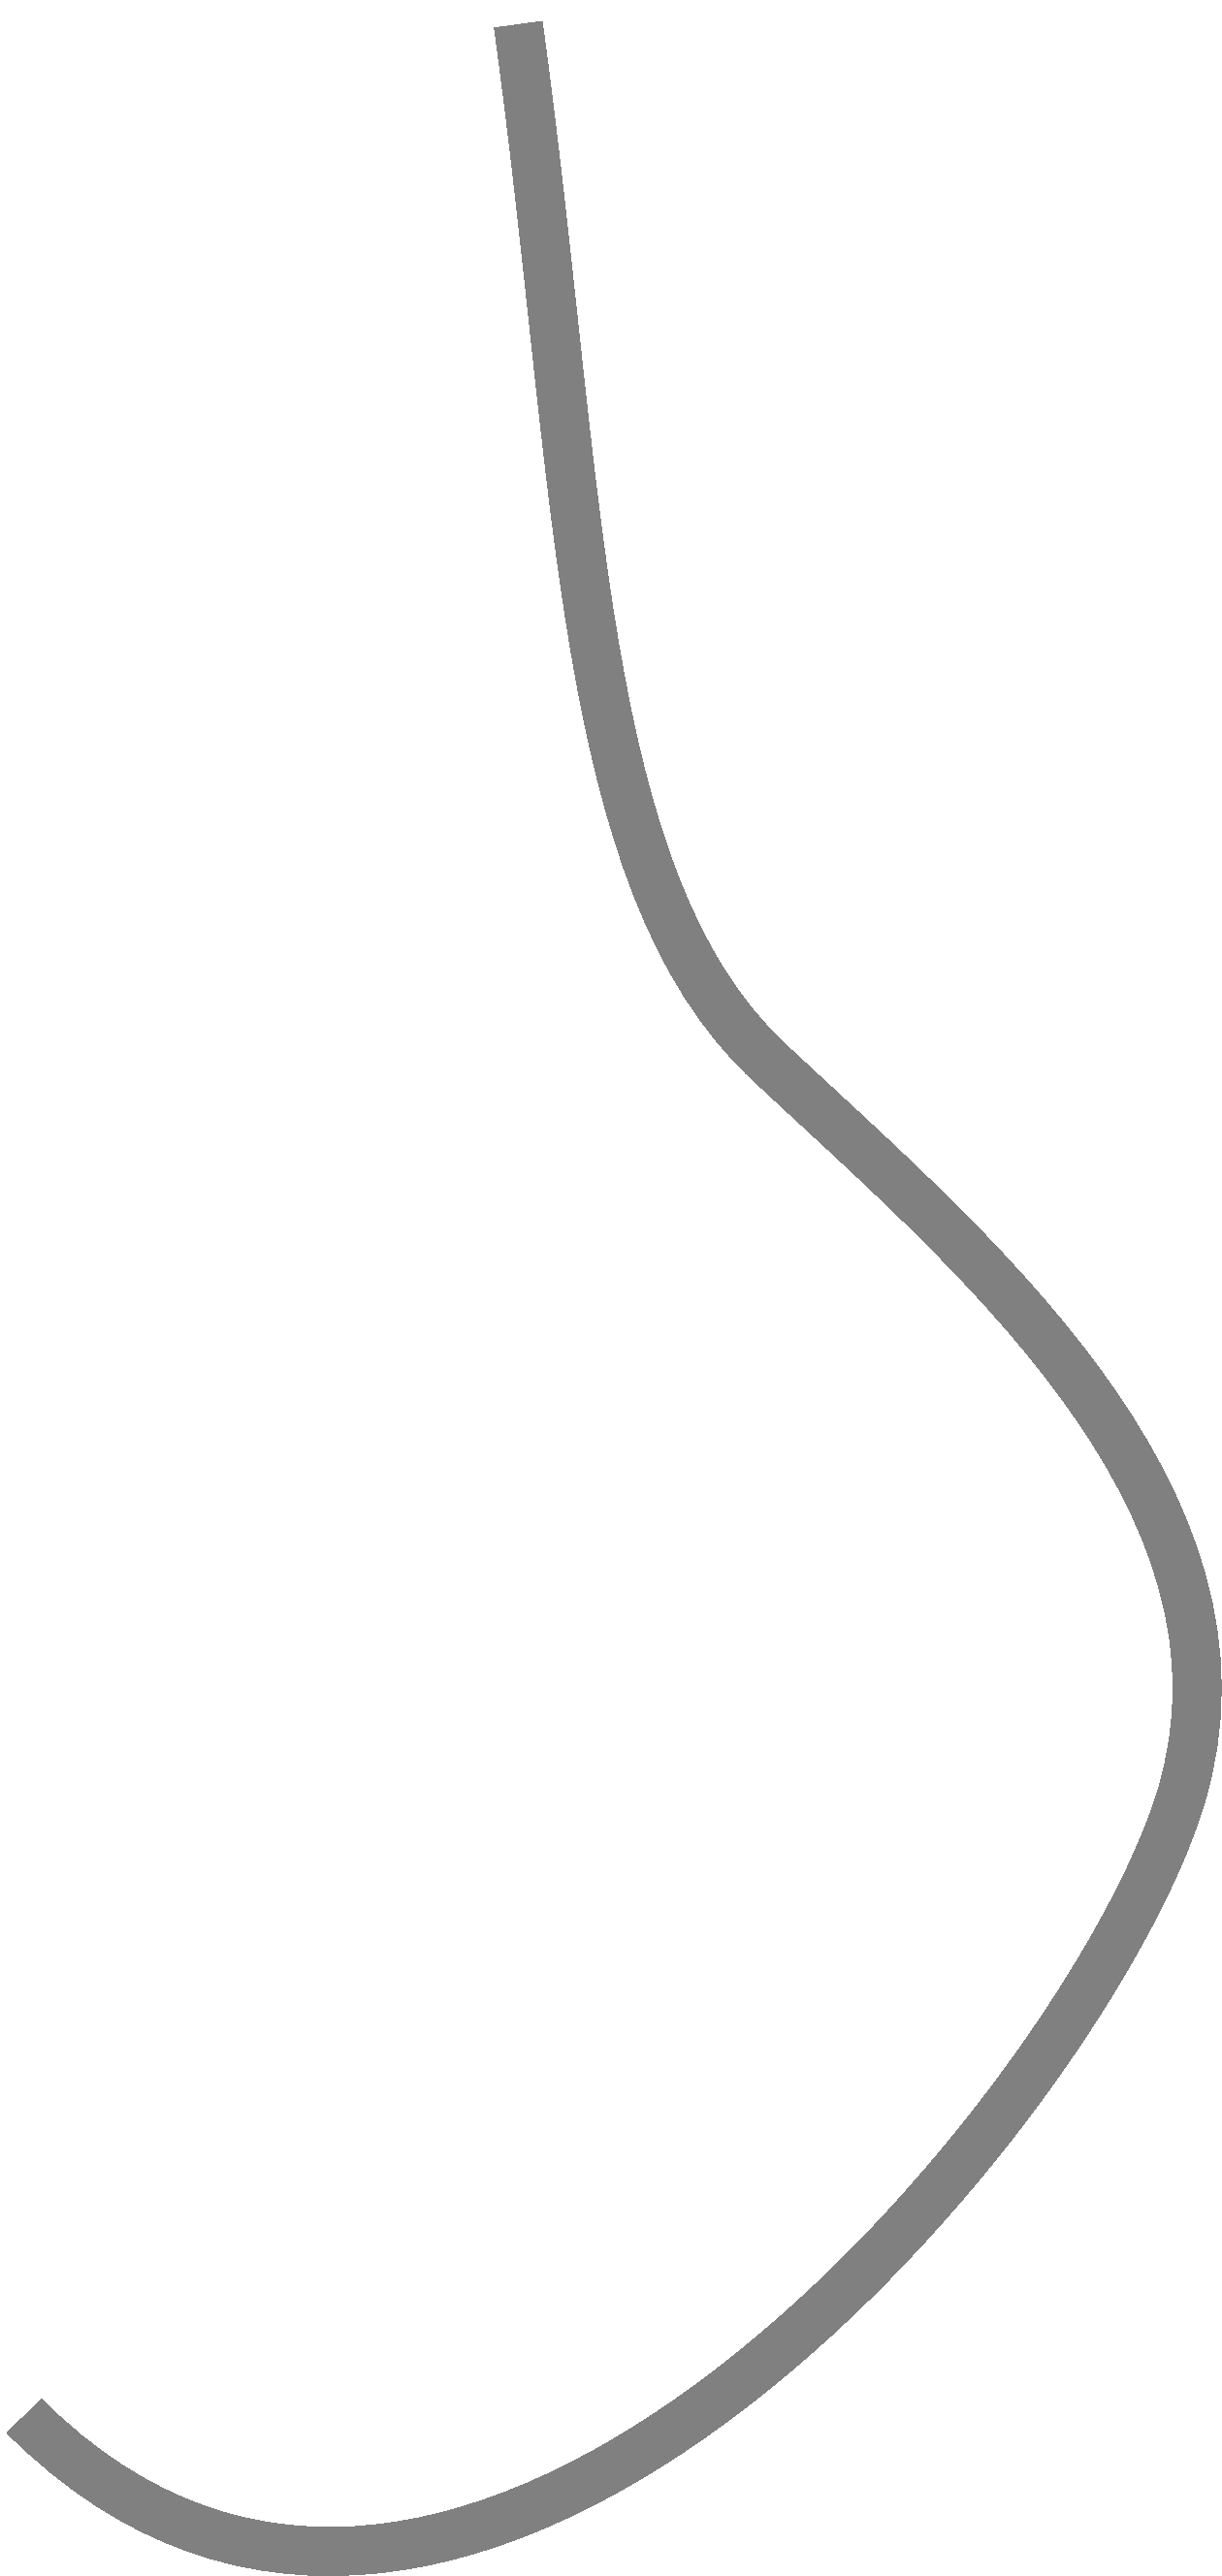
\includegraphics[height=4em]{images/fluxsurface.pdf}
\end{center}
and suppose we are told that there's a flux of momentum through it, from left to right, {having the following direction and orientation:\noprelistbreak%
\begin{center}
  
\includegraphics[height=4em]{images/vec_NW.pdf}
\end{center}
}
\noindent with magnitude \textcolor{blue}{\qty{6}{N}}.

\begin{warning}[Vector flux and crossing direction are two separate things]
  The vector that represents the flux, like the one above, and the surface-crossing direction, say left-to-right, are completely separate and independent things. In particular, they can have completely different directions.
\end{warning}

\smallskip

We could visualize the flux above as follows:
\begin{center}
  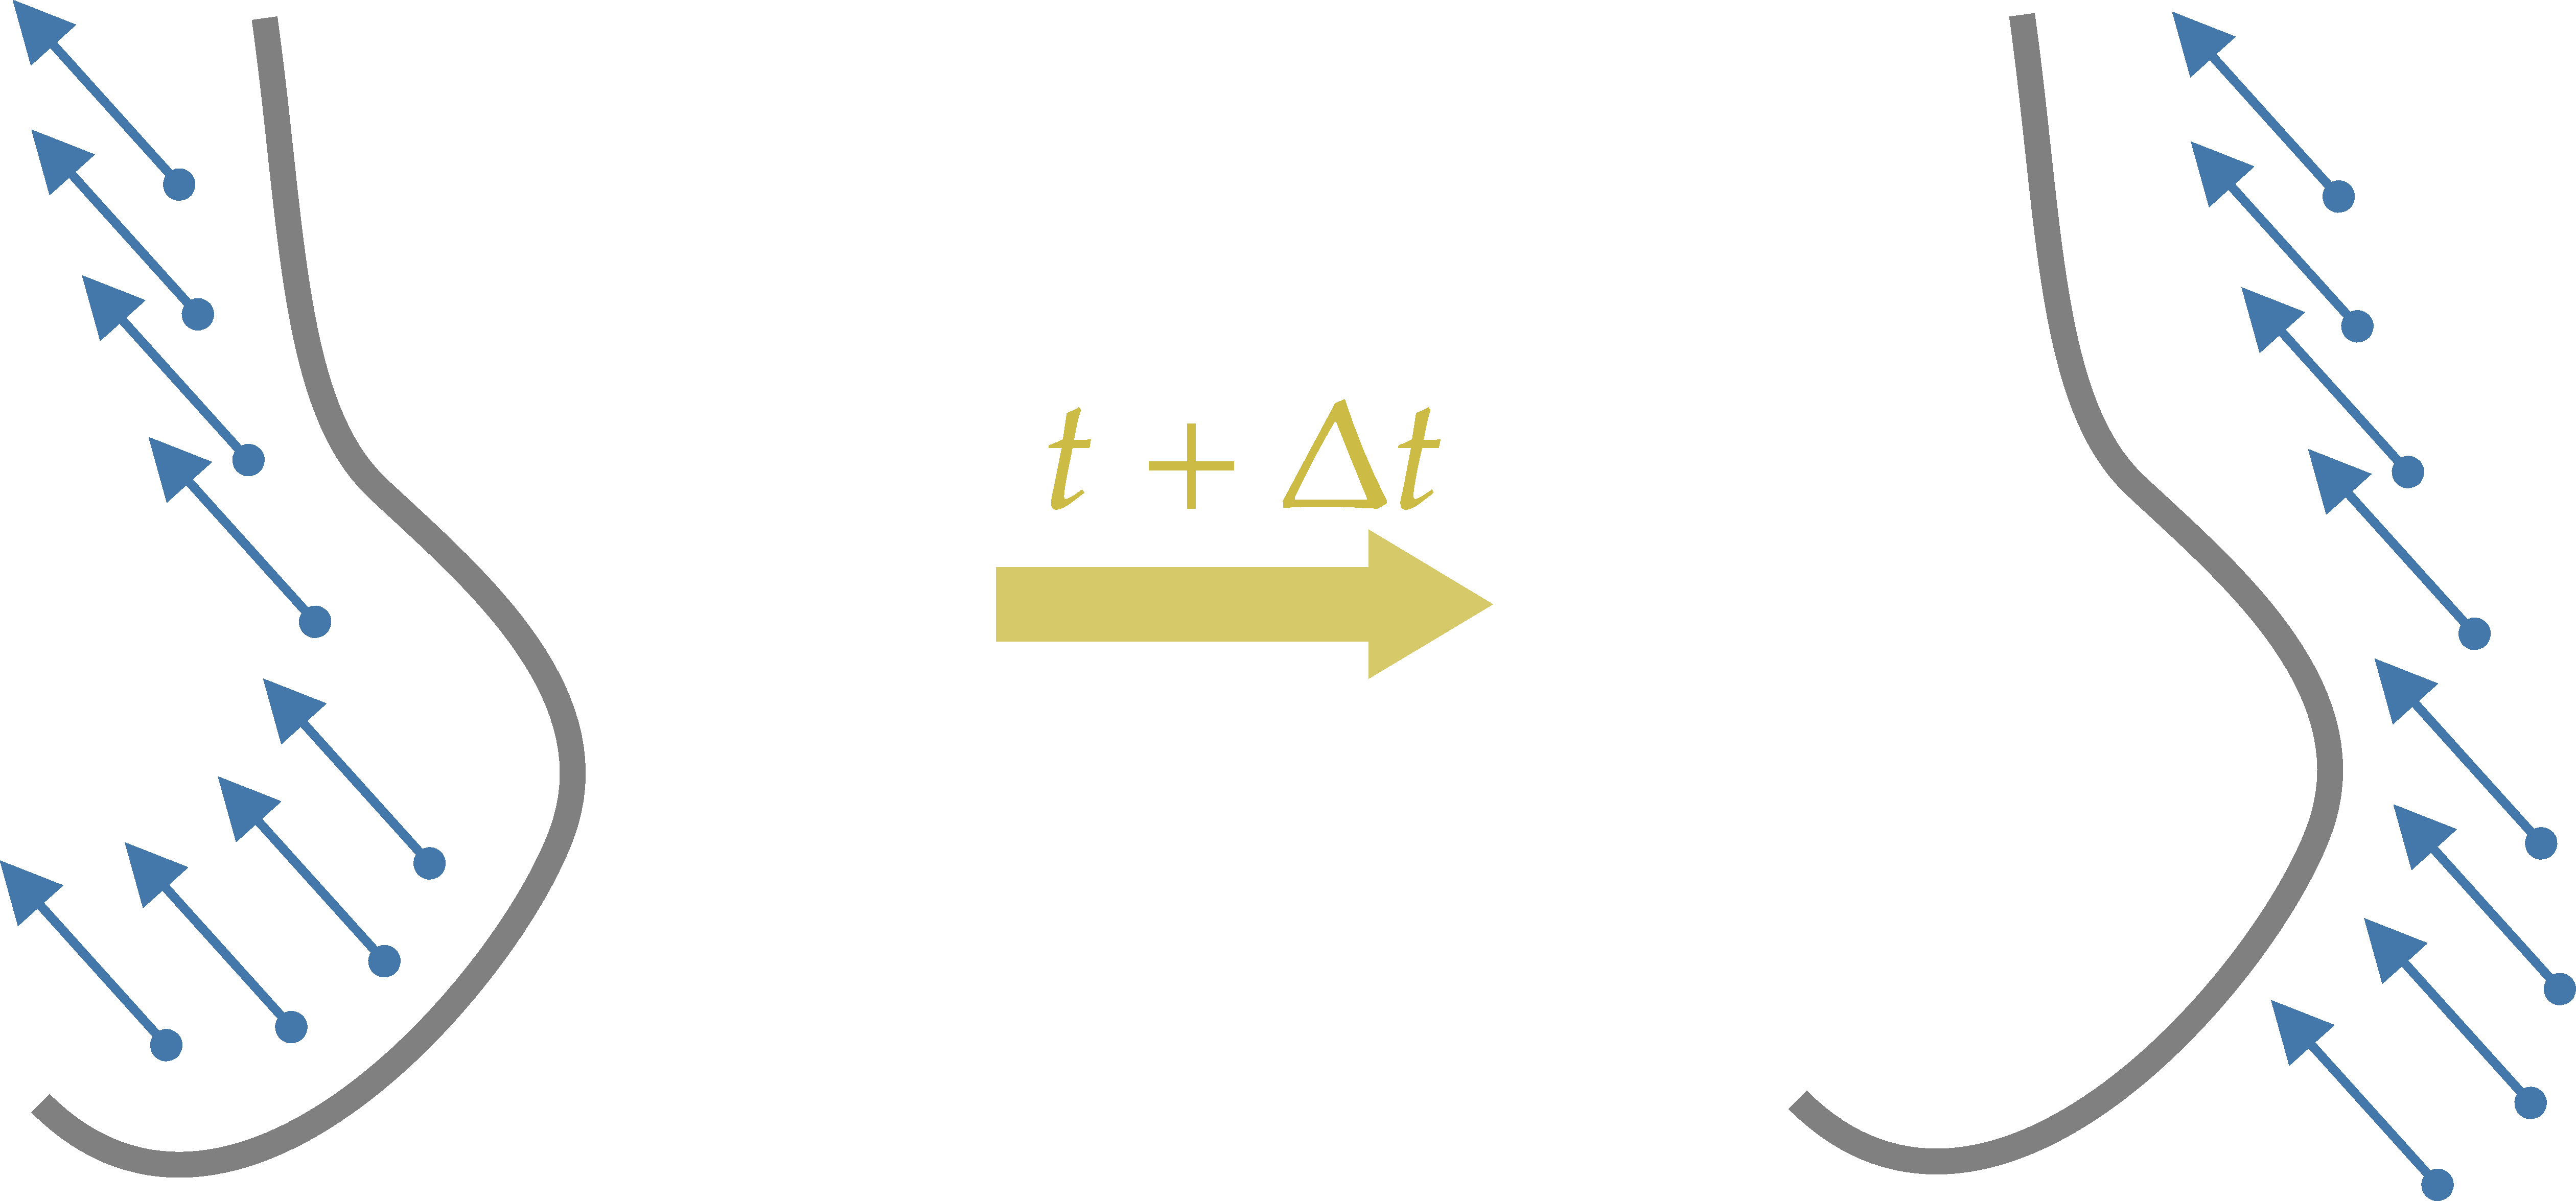
\includegraphics[height=5em]{images/flux_vector_shift.pdf}
\end{center}
with the familiar warning that the surface could be moving. But the following visualization also corresponds to exactly the same flux:
\begin{center}
  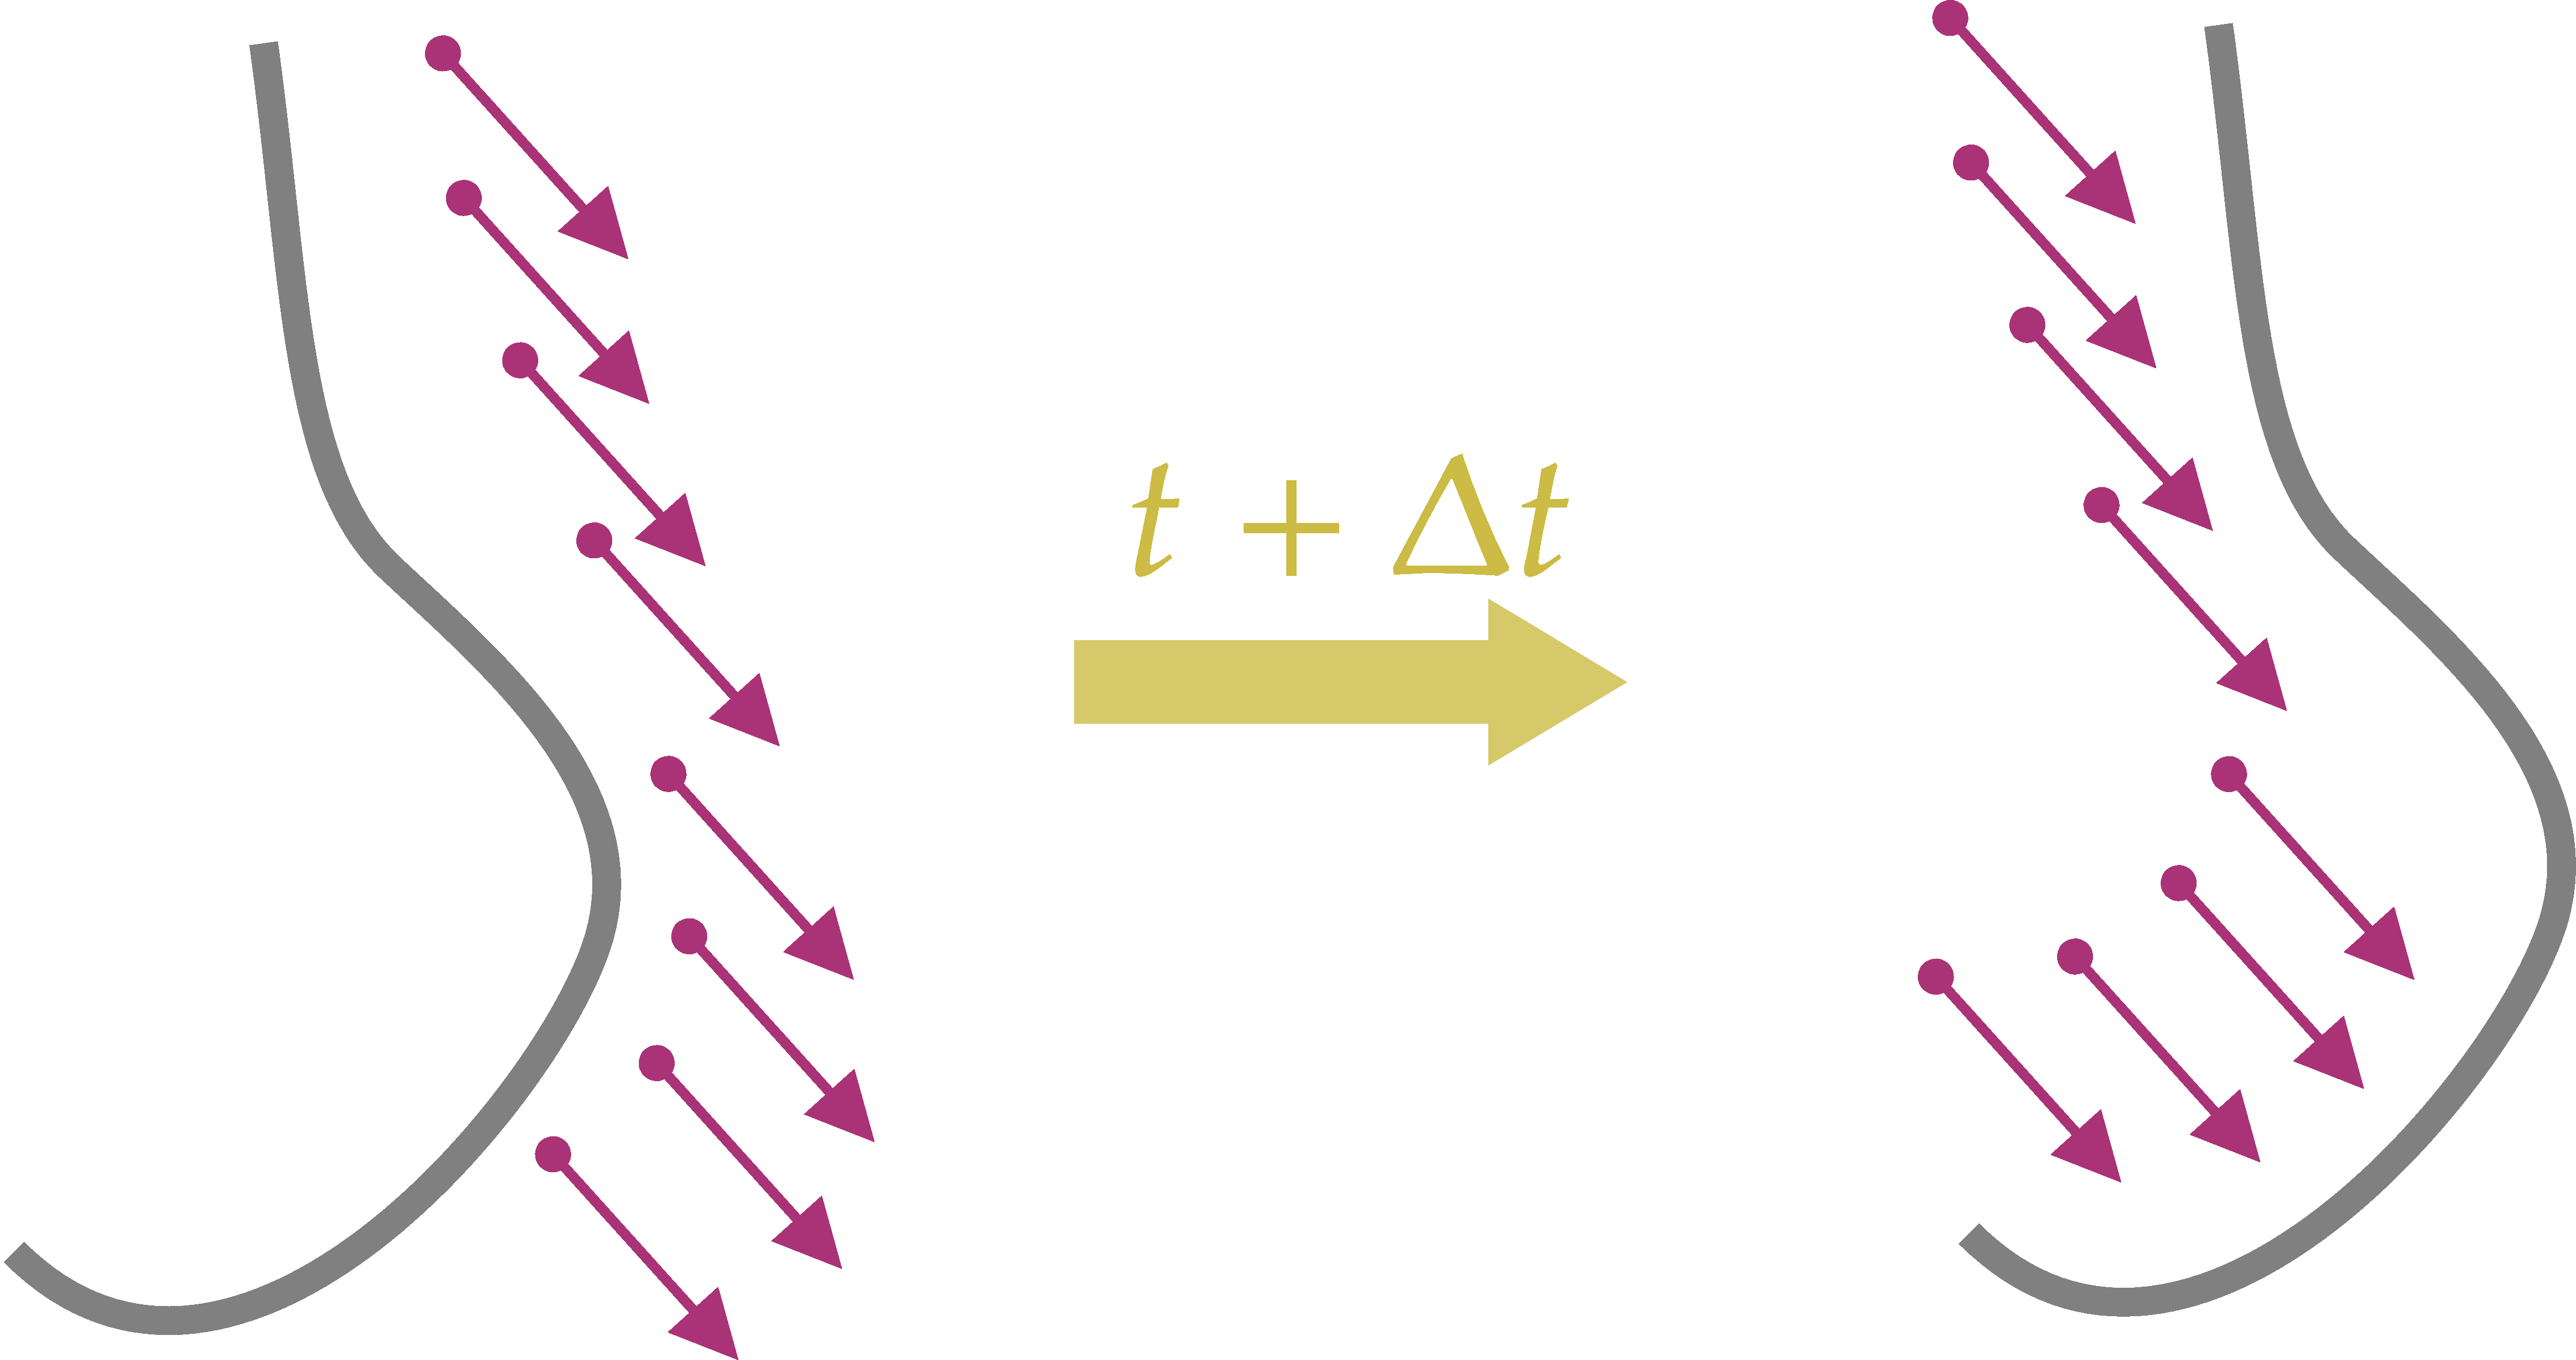
\includegraphics[height=5em]{images/flux_vector_shift_neg.pdf}
\end{center}
What happens in either illustration is that there's a change equal to a vectorial amount\enspace
\includegraphics[align=c,height=2em]{images/vec_NW.pdf}\enspace of magnitude \qty{6}{N} on the \emph{right} of the surface, and a change equal to the \emph{opposite} vectorial amount\enspace
\includegraphics[align=c,height=2em]{images/vec_SE.pdf}\enspace of the same magnitude on the \emph{left} of the surface.

{A less misleading representation of the flux in our example could therefore be like this:\noprelistbreak%
  \begin{center}
    \includegraphics[height=7em]{images/flux_vec_both.pdf}
  \end{center}
}
\noindent This picture says that there's a momentum change of a particular direction, orientation, magnitude on the left side of the surface, and an opposite momentum change on the right side of the surface. Note that \textbf{the vectors indicated on the two sides must be opposite and have equal magnitude}, otherwise the picture doesn't make sense.

An animated representation or mental visualization can also be quite illuminating. You can see one \furl{https://pglpm.github.io/7wonders/media/vectorfluxanimation.webp}{at this link}.

\nonosection{The symmetry of fluxes}
\label{nsec:fluxes_symmetry}

Our discussion about fluxes of scalar and vector quantities, and their graphical representation, for instance
\begin{center}\hspace*{\fill}
  \includegraphics[height=7em]{images/flux_both.pdf}
  \hfill \includegraphics[height=7em]{images/flux_vec_both.pdf} \hspace*{\fill}
\end{center}
shows an important mathematical and physical symmetry of the flux of a quantity.

The \emph{sign} of the flux is determined by the direction in which we imagine to cross the surface. In the first picture above, if we are imagining to cross the surface from left to right, then the energy flux is \textcolor{blue}{\qty{+4}{J/s}}; and if we are imagining to cross the surface from right to left, then the energy flux is \textcolor{purple}{\qty{-4}{J/s}}. Analogously for the vector flux in the second picture above, where the minus sign corresponds to flipping the vector.

The crossing direction is arbitrary, completely left to us (just like the surface itself is arbitrary). It is therefore always important, when we report a flux through a surface, to state which crossing direction we have agreed upon.

We can state this symmetry as follows:
\marginpar{\footnotesize\raggedright%
  \color{mpcolor}\enquote{\emph{%
        \langnohyph{LEX~III. Actioni contrariam semper \amp\ {\ae}qualem esse reactionem\,: sive corporum duorum actiones in se mutuo semper esse {\ae}quales \amp\ in partes contrarias dirigi.}}}
        \\[\jot]
        \enquote{\emph{LAW~III. To every action there is always opposed an equal reaction: or, the mutual actions of two bodies upon each other are always equal, and directed to contrary parts.}}
    \\\sourceatright{\cites{newton1687}} %\cites{newton1687_t1974}
}%
\begin{definition}{Every flux is the same as the opposite flux in the opposite direction}
  A flux  in a particular surface-crossing direction is equivalent to a flux of opposite sign in the opposite crossing direction.
\end{definition}
This statement may sound familiar. Indeed \emph{it includes Newton's famous third law, the \enquote{principle of action and reaction}, as a special case}. Newton's third law is the expression of the symmetry of vector fluxes, but for the specific case of the flux of momentum, that is, force. Now we see that this property is more general: it applies not only to force, but also to the flux of angular momentum (torque), and to the flux of scalar quantities as well.

\bigskip

% \mynotew{Section on not making conclusions about a flux through a surface from flux through another}

----

In the previous section we saw that a balance law can be used to predict how the density of a quantity changes with time. But we also saw that in order to make such prediction we need to already know what the \emph{future} fluxes of the quantity will be, throughout the region of interest. This doesn't sound like a great achievement: to predict the future, we need the future. The situation doesn't improve if we have two or more quantities that satisfy balance laws: we shall need to know in advance the fluxes of each.

It turns out, however, that there are physical laws which \emph{relate the densities of some quantities to the fluxes of others}. Such relations can potentially allow us to calculate the time evolution without knowing the fluxes in advance. Roughly, the basic idea is as follows: From the density of one quantity, we calculate the fluxes of the second quantity, and use them to predict its density at a later time. Once we know this density, we use it to calculate the new fluxes of the first quantity, and therefore its density at a later time; and so on. This cross-prediction does not fully eliminate the necessity of specifying some future quantities in advance; but the remaining ones that we need to specify are often in our control. Indeed this is how we can predict how a physical system will respond to influences controlled by us.

Physical laws of this kind turn out not to be universal: they depend on, or are \furl{https://www.merriam-webster.com/dictionary/constitutive}{\enquote*{constitutive}} of, the particular physical phenomenon and the physical theory being used. For this reason they are called \textbf{constitutive relations} or \textbf{constitutive equations}. In some fields they are called \textbf{closure equations}, because they allow us to \enquote{close} the system of balance equations in such a way that it can be used for future predictions without knowing in advance the future value of some quantities.

Constitutive relations express the diversity that we observe around us, for example the different behaviours of a drop of water, which obeys some constitutive relations, as compared with a block of wood, which obeys others. They also mark the difference between specialized or approximate physical theories, for example between Newtonian mechanics, which is based on particular approximate constitutive relations, and General Relativity, which is based on different and more exact constitutive relations. Depending on the specific scientific field you'll work in, you'll learn some constitutive relations in more detail than others.

Constitutive relations come in a great variety of mathematical forms. Some of them are simple algebraic relations between the density of one quantity and the flux of another. Others involve spatial or time derivatives. Other still involve integrals in space or in time.% ; the latter give rise to physical phenomena that posses \enquote{memory}.

\mynotew{Add examples of laws that reduce to the balances: Bernoulli, Poynting?, mechanical-energy-work theorem}

----

The control volumes for the two bodies contain amounts of momentum $\yPa = \yMa\,\yva$, $\yPb=\yMb\,\yvb$, according to the \autoref{sec:bal_momentum_Newton}{Newtonian constitutive equation}. We assume no momentum fluxes across the closed control surfaces, except across the narrow parts in contact with the control volume of the spring, where the momentum \textbf{in}fluxes are $\yFab$ for body $a$ and $\yFba$ for body $b$ (see side picture below). We are using this notation for the fluxes: \enquote*{$\yFab$} means that it's the influx into body $a$, coming from the spring that connects it to body $b$.

If we consider gravity effects, the control volumes of the two bodies might also have constant momentum supplies $\yGa=\yMa\,\yg$, $\yGb=\yMb\,\yg$ according to the \autoref{def:gravity_surface}{constitutive equation for gravitational force}.  Let's omit these supplies for simplicity.

The control volume for the spring contains no momentum $\yP$ and has no supply $\yG$, according to the Hookean constitutive properties. At the two narrow surfaces in contact with the bodies (see side picture), it has momentum \textbf{in}fluxes $-\yFab$ and $-\yFba$, owing to the \autoref{def:symmetryflux}{symmetry of fluxes}. The total momentum influx is therefore $\yF=-\yFab-\yFab$ by extensivity.

Note that all the quantities so far, except the masses, depend on the time $t$.

The Hookean constitutive relation~\eqref{eq:hooke} says that the momentum \textbf{ef}flux across one surface, say the one in contact with body $a$, must be
\begin{equation*}
  \yFab = -k\,(\yra-\yrb)
\end{equation*}
because $\yra-\yrb$ is the main length of the control volume for the spring.

Now let's apply balances and constitutive equations to the three control volumes:
  \begin{equation*}
 \begin{aligned}
&\text{\footnotesize momentum balance} &\quad&\frac{\di\yPa(t)}{\di t} = \yFab(t) + \yGa(t)
      \\[\jot]
&\text{\footnotesize const. equation} &\quad&\yPa(t) = \yMa\yva(t)
      \\[\jot]
&\text{\footnotesize boundary condition} &\quad&\yGa(t) = 0
    \end{aligned}
  \end{equation*}

  \begin{equation*}
 \begin{aligned}
&\text{\footnotesize momentum balance} &\quad&\frac{\di\yPb(t)}{\di t} = \yFba(t) + \yGb(t)
      \\[\jot]
&\text{\footnotesize const. equation} &\quad&\yPb(t) = \yMb\yvb(t)
      \\[\jot]
&\text{\footnotesize boundary condition} &\quad&\yGb(t) = 0
    \end{aligned}
  \end{equation*}

  \begin{equation*}
 \begin{aligned}
&\text{\footnotesize momentum balance} &\quad&\frac{\di\yP(t)}{\di t} = \yF(t) + \yG(t)
      \\[\jot]
&\text{\footnotesize total influx by extensivity} &\quad&\yF(t) = -\yFab(t) - \yFba(t)
      \\[\jot]
&\text{\footnotesize Hooke const. equation} &\quad&\yP(t) = 0
      \\[\jot]
&\text{\footnotesize Hooke const. equation} &\quad&\yG(t) = 0
      \\[\jot]
&\text{\footnotesize Hooke const. equation} &\quad&\yFab(t) = -k\,[\yra(t)-\yrb(t)]
    \end{aligned}
  \end{equation*}



----
LINKS
nuclear reaction:
https://www.britannica.com/technology/nuclear-reactor/Liquid-metal-reactors
https://www.energy.gov/ne/nuclear-fuel-facts-uranium
https://www.energy.gov/ne/articles/nuclear-101-how-does-nuclear-reactor-work
https://www.world-nuclear.org/information-library/nuclear-fuel-cycle/introduction/physics-of-nuclear-energy.aspx
http://large.stanford.edu/courses/2011/ph241/grayson1/ % boron

----
density: Q/V
flux, flow: Q(area)/t
flux density: Q(area)/(A.t)
or surface ... density

$$
P_{x} = \yM\,v_{x} +
\frac{1}{c^{2}}\bigl(
\yH_{x} +
\tfrac12 \yM\,v_{x}\,\yv^{2}
+ \yM\,v_{x}\,\yE/V
+ 3\,\yM\,g\,v_{x}
\bigr)
$$

$$
\begin{gathered}
  \yP(t+\Dt) = \yP(t) + \int_{t}^{\mathrlap{t+\Dt}}\!\yF(t)\,\di t + \int_{t}^{\mathrlap{t+\Dt}}\!\yG(t)\,\di t
  \\
  \yF(t) = 0
  \\
  \yG(t) = \dotso
\end{gathered}
$$

$$
\begin{aligned}
  &\yP_a(t+\Dt) = \yP_a(t) + \int_{t}^{\mathrlap{t+\Dt}}\!\yF_a(t)\,\di t + \int_{t}^{\mathrlap{t+\Dt}}\!\yG_a(t)\,\di t
  \\
  &\yP_b(t+\Dt) = \yP_b(t) + \int_{t}^{\mathrlap{t+\Dt}}\!\yF_b(t)\,\di t + \int_{t}^{\mathrlap{t+\Dt}}\!\yG_b(t)\,\di t
  \\
  &\yF_{b}(t) = -\yF_{a}
  \\
  &\yF_{a}(t) = -k\, (z_{a}-z_{b})
  \\
  &\yP_{a} = \yMa v_{a}
  \\
  &\yP_{b} = \yMb v_{b}
  \\
  &\yG_{a}(t) = \dotso
  \\
  &\yG_{b}(t) = \dotso
\end{aligned}
$$

$$
\begin{aligned}
  &\yP_a(t+\Dt) = \yP_a(t) + \int_{t}^{\mathrlap{t+\Dt}}\!\yF_a(t)\,\di t + \int_{t}^{\mathrlap{t+\Dt}}\!\yG_a(t)\,\di t
  \\
  &\yP_b(t+\Dt) = \yP_b(t) + \int_{t}^{\mathrlap{t+\Dt}}\!\yF_b(t)\,\di t + \int_{t}^{\mathrlap{t+\Dt}}\!\yG_b(t)\,\di t
  \\
  &\yP_c(t+\Dt) = \yP_c(t) + \int_{t}^{\mathrlap{t+\Dt}}\!\yF_c(t)\,\di t + \int_{t}^{\mathrlap{t+\Dt}}\!\yG_c(t)\,\di t
  \\
  &\yF_{b}(t) = -\yF_{a}
  \\
  &\yF_{a}(t) = -k\, (\yr_{a}-\yr_{b})
  \\
  &\yP_{a} = \yMa \yv_{a}
  \\
  &\yP_{b} = \yMb \yv_{b}
  \\
  &\yG_{a}(t) = \dotso
  \\
  &\yG_{b}(t) = \dotso
\end{aligned}
$$

$$
\begin{aligned}
  &\yP_a(t+\Dt) = \yP_a(t) + \int_{t}^{\mathrlap{t+\Dt}}\!\yF_a(t)\,\di t + \int_{t}^{\mathrlap{t+\Dt}}\!\yG_a(t)\,\di t
  \\
  &\yP_b(t+\Dt) = \yP_b(t) + \int_{t}^{\mathrlap{t+\Dt}}\!\yF_b(t)\,\di t + \int_{t}^{\mathrlap{t+\Dt}}\!\yG_b(t)\,\di t
  \\
  &\yP_c(t+\Dt) = \yP_c(t) + \int_{t}^{\mathrlap{t+\Dt}}\!\yF_c(t)\,\di t + \int_{t}^{\mathrlap{t+\Dt}}\!\yG_c(t)\,\di t
  \\
  &\yF_{ba}(t) = -\yF_{ab}
  \\
  &\yF_{ca}(t) = -\yF_{ac}
  \\
  &\yF_{bc}(t) = -\yF_{cb}
  \\
  &\yF_{ab}(t) = -k\, (\yr_{a}-\yr_{b})
  \\
  &\yF_{ac}(t) = -k\, (\yr_{a}-\yr_{c})
  \\
  &\yF_{cb}(t) = -k\, (\yr_{c}-\yr_{b})
  \\
  &\yP_{a} = \yMa \yv_{a}
  \\
  &\yP_{b} = \yMb \yv_{b}
  \\
  &\yP_{c} = \yMb \yv_{c}
  \\
  &\yG_{a}(t) = \dotso
  \\
  &\yG_{b}(t) = \dotso
  \\
  &\yG_{c}(t) = \dotso
\end{aligned}
$$


$$
\yF_{\text{Earth-Sun}} =
-G\frac{\yM_{\text{Sun}}\,\yM_{\text{Earth}}}{\abs{\yr_{\text{Earth}} - \yr_{\text{Sun}}}^2}\,
 \biggl[
 \tfrac{\yr_{\text{Earth}} - \yr_{\text{Sun}}}{\abs{\yr_{\text{Earth}} - \yr_{\text{Sun}}}}
 +2\,
 \yv_{\text{Earth}} \times \Bigl(\yv_{\text{Sun}} \times
 \tfrac{\yr_{\text{Earth}} - \yr_{\text{Sun}}}{\abs{\yr_{\text{Earth}} - \yr_{\text{Sun}}}}
\Bigr)
 \biggr]
 $$

 ------------

 % We shall see that the energy content within a control volume and the energy flux through a control surface can depend on many other quantities like matter content and flux, momentum content and flux, electric charge and electromagnetic field, and auxiliary quantities such as temperature. This dependence can be wildly different, depending on the physical phenomenon.

Keep in mind that these expressions denote particular mathematical parts and don't really mean that energy can ultimately be divided that way.

In the previous section we divided energy into \enquote*{internal}, \enquote*{kinetic}, and \enquote*{gravitational}. That division, however, comes from different references for the definition of energy and does not imply separate dependence on matter, electromagnetic field, and so on. Internal, kinetic, and gravitational energy will in general all depend on all other relevant quantities.

% No, according to our present knowledge. First of all, recall that \autoref{wa:conservation}{many texts use the term \enquote*{conservation} in the sense of \enquote*{balance}} as defined in the present notes. So when they speak of \enquote{energy conservation} they don't exclude the presence of an energy supply, the creation of energy within a volume.
% In fluid mechanics, for instance, we usually describe physical phenomena using the internal-energy definition, and as mentioned above this energy definition satisfies a balance law, not a conservation law.



\end{itemize}
We thus have the relation
\begin{multline*}
  \label{eq:energy_division}
  % \yE = \yU + \yEk + \yEp
  \text{\enquote*{coordinate} energy} ={}\\
  \text{internal energy} +
  \text{kinetic energy} +
  \text{gravitational potential energy}
\end{multline*}

% %
% \marginpar{\vspace{\baselineskip}%
%   \footnotesize\flushleftright\color{mpcolor}%
%   \enquote{\emph{a distinction is made between the principle of conservation of energy and the first law of thermodynamics, the two being identical only when matter is at rest}} \sourceatright{\cites{eckart1940c}}%
% }%


% It is this variety of choices that leads to the variety of \enquote{kinds} of energy.
% %
% \marginpar{\vspace{\baselineskip}%
% \footnotesize\flushleftright\color{red}%
% \faIcon{exclamation-circle}\enspace Some texts say that different definitions of energy correspond to different choices of coordinate systems, but that is not correct.%
% }%

\nonosection{The Newtonian balance of energy for matter}
\label{sec:newton_balance_energy}

We have thus far discussed two general families of constitutive relations, one for the energy content $\yE$, formula~\eqref{eq:thermodynamic_energy} and one for the energy flux $\yH$, formula~\eqref{eq:heat_power}, which can be applied to a control volume:
\begin{equation*}
  \begin{gathered}
    \yE = \yU + \tfrac12 \yM \yv^{2} + \yM g z
    \\
    \yH = \yQ + \yF\cdot\yv
  \end{gathered}
\end{equation*}
Let us recall the conditions under which they are valid:
\begin{itemize}[nosep]
\item matter present within and directly outside the control volume
\item control volume small enough  to consider the velocity $\yv$ the same throughout
\item no matter flux through the surface of the control volume
\item no electric charges or electromagnetic fields
\item Newtonian approximation, and close to the Earth's surface
\end{itemize}
We also said that \autoref{item:energy_no_supply}{our definition of energy approximately satisfies a conservation law}, so the energy supply is zero: $\yR=0$.

We can insert these expressions for $\yE,\yH,\yR$ in the equation of energy balance~\eqref{eq:bal_energy}, obtaining these specialized integral and differential forms of the energy balance:
\begin{equation}
  \label{eq:bal_energy_newton}
  \begin{gathered}
      \begin{multlined}[0.9\linewidth]
        \yU(\ytf) + \tfrac12 \yM \yv^{2}(\ytf) + \yM g z(\ytf) ={}\\
        \yU(\yti) + \tfrac12 \yM \yv^{2}(\yti) + \yM g z(\yti)
        + \int_{\yti}^{\ytf}\!\!
        \bigl[\yQ(t) + \yF(t)\cdot\yv(t)\bigr]\,\di t
      \end{multlined}
    \\[4\jot]
      \frac{\di\bigl[\yU(t) + \tfrac12 \yM \yv^{2}(t) + \yM g z(t)\bigr]}{\di t} =
      \yQ(t) + \yF(t)\cdot\yv(t)
  \end{gathered}
\end{equation}





\nonosubsection{The \enquote{work-energy theorem}}
\label{sec:workenergy_thm}

Let us consider, at a particular time $t$, a control volume containing a body of matter with total \masse\ $\yM$ and having the same velocity $\yv(t)$ everywhere. In other words, if we measure the velocity of matter in a small portion of the volume, we find $\yv(t)$; if we measure the velocity in another small portion, we find $\yv(t)$ as well; and so on.

In Newtonian approximation and in absence of charges and electromagnetic fields, the total momentum in the control volume is $\yP(t)=\yM\yv(t)$. Suppose that there's a total influx of momentum $\yF$ through the surface of the control volume; and there's a constant momentum supply $\yG(t) = \yM g\, [0,0,1]$ from gravity. We have chosen coordinates $(x,y,z)$ with $z$ pointing upwards.

The differential form of the balance of momentum is therefore
\begin{equation*}
  \begin{aligned}[b]
    \frac{\di\yP(t)}{\di t} &= \yF(t) + \yG(t)
\\
    \frac{\di\yM \yv(t)}{\di t} &= \yF(t) + \yM g\, [0,0,1]
  \end{aligned}
\end{equation*}
Multiply the left and right sides of this equation by $\yv(t) = [v_{x}(t), v_{y}(t), v_{z}(t)]$, using the dot-product:
\begin{equation}
    \label{eq:balance_mom_wethm}
  \frac{\di\yM \yv(t)}{\di t} \cdot \yv(t) = \yF(t)\cdot \yv(t) + \yM g\, [0,0,1]\cdot \yv(t)
\end{equation}

Now note the following equalities:
\begin{equation*}
  \begin{gathered}
    [0,0,1]\cdot\yv(t) = [0,0,1]\cdot [v_{x}(t), v_{y}(t), v_{z}(t)] = v_{z}(t)
    = \frac{\di z(t)}{\di t}
    \\[2\jot]
    \frac{\di \yv(t)^{2}}{\di t} =
  \frac{\di[\yv(t) \cdot \yv(t)]}{\di t} =
  \frac{\di\yv(t)}{\di t} \cdot \yv(t) + \yv(t)\cdot \frac{\di\yv(t)}{\di t}
  =
  2\frac{\di\yv(t)}{\di t} \cdot \yv(t)
  \end{gathered}
\end{equation*}
\marginpar{\vspace{-3\baselineskip}%
\footnotesize\flushleftright\color{mpcolor}%
the equalities come from the product rule of the derivative and the commutativity property of the dot-product%
}%
Multiplying the first set of equalities above by the constant $\yM g$, and the second by the constant $\tfrac12 \yM$, we find
\begin{equation*}
  \begin{gathered}
    \yM g\,[0,0,1]\cdot\yv(t)
    = \frac{\di\yM g z(t)}{\di t}
    \\[2\jot]
    \frac{\di \tfrac12 \yM \yv(t)^{2}}{\di t} =
  \frac{\di\yM\yv(t)}{\di t} \cdot \yv(t)
  \end{gathered}
\end{equation*}
We can now replace these equalities in formula~\eqref{eq:balance_mom_wethm}, the balance of momentum that we dot-multiplied by the velocity, and bring the last term on the right to the left. We obtain this equation:
\begin{equation}
  \label{eq:wethm}
  \frac{\di\bigl[\tfrac12 \yM \yv(t)^{2} + \yM g z(t)\bigr]}{\di t} =
  \yF(t)\cdot \yv(t)
\end{equation}
which is usually called \enquote{\textbf{work-energy theorem}}.

The equation above is very peculiar. On the left side, within the time derivative, w see the kinetic energy and gravitational potential energy; so this is almost the full energy content $\yE$ given by the general constitutive relation~\eqref{eq:thermodynamic_energy}, except that the internal energy $\yU$ is missing. On the right side we see the mechanical power; so this is almost the full energy flux $\yH$ given by the general constitutive relation~\eqref{eq:heat_power}, except that the heat flux $\yQ$ is missing.

$$\yFn = \frac{\di P_{z}}{\di t} - \bigl(F_{z}\bigr)_{\text{other}} - G_{z}$$


------


In \chap\,\ref{cha:stuff} we introduced seven main quantities in terms of which we describe physical phenomena. How do we describe the patterns, regularities, and diversities that we observe in these phenomena? This is the role of \emph{physical laws}. Different physics formalisms express physical laws in different ways, even if the actual physical phenomenon is exactly the same. In the formalism that we are using we distinguish between two kinds of physical laws:
\begin{definition}{Two kinds of physical laws}
  \begin{itemize}
  \item\textbf{Fundamental laws} represent universal patterns that we observe everywhere, and that are taken as the basic mathematical equations in a physical theory.
    % We shall see that there is a set of seven fundamental laws that apply on every known scale of space and time, and also across different physical theories.

  \item\textbf{constitutive relations} or \textbf{properties} only apply to particular phenomena, only on particular time \amp\ space scales, only in particular theories. They express the diversity that we observe around us, and different kinds of approximations that we use in describing physical phenomena.
  \end{itemize}
\end{definition}

This distinction it's important. The fundamental laws can be applied with some confidence to every new phenomenon we observe, and often allow us to make predictions of at least a qualitative character. As far as we know there is a very small number of fundamental laws. We only modify them as a last resort (and so far this has rarely or never been necessary). We have a lot of freedom in modifying constitutive relations instead, and in proposing new ones to account for newly observed physical phenomena.

------

baryonic and leptonic matter, independently of the kinds into which it can be classified, is always conserved.


Often the classification is related to whether the different kinds of matter under consideration are at least approximately \autoref{sec:balance_intro}{conserved}, as we'll discuss later.

In everyday phenomena not involving \furl{https://www.iaea.org/newscenter/news/what-are-radioactive-sources}{radioactivity}
% \url{https://www.britannica.com/science/radioactivity}
or \furl{https://www.iaea.org/newscenter/news/what-is-nuclear-energy-the-science-of-nuclear-power}{nuclear energy},
% \url{https://www.britannica.com/science/nuclear-fission}
matter is classified into different kinds, approximately corresponding to the non-\furl{https://www.ciaaw.org/radioactive-elements.htm}{radioactive} chemical elements: \furl{https://pubchem.ncbi.nlm.nih.gov/element/Hydrogen}{hydrogen}, \furl{https://pubchem.ncbi.nlm.nih.gov/element/Helium}{helium}, \furl{https://pubchem.ncbi.nlm.nih.gov/element/Lithium}{lithium}, and so on. %\furl{https://doi.org/10.1351/goldbook.C01022}{}.
Note that some common everyday devices, such as smoke detectors, do involve radioactivity.

In phenomena involving radioactivity or nuclear energy, the different kinds of matter correspond approximately to \furl{http://hyperphysics.phy-astr.gsu.edu/hbase/Particles/hadron.html\#c6}{\emph{baryons}},
% \url{https://www.britannica.com/science/baryon}},
like protons and neutrons; and \furl{http://hyperphysics.phy-astr.gsu.edu/hbase/Particles/lepton.html\#c1}{\emph{leptons}},
% \url{https://www.britannica.com/science/lepton}},
such as electrons. In particle physics, even more subtle classifications of matter are made, into kinds that seem to be conserved, like electronic-leptons, muonic-leptons, and others. This kind of research is still open, but it seems that the total amount of baryonic and leptonic matter, independently of the kinds into which it can be classified, is always conserved. Note that we're using the term \enquote*{matter} in a sense that includes anti-matter, such as positrons.

----

Consider these two representations:\noprelistbreak
\begin{center}\label{fig:scalar_fluxes}
  \bigskip
\hspace*{\fill}\includegraphics[height=6em]{images/flux_plus5c.pdf}
\hfill\includegraphics[height=6em]{images/flux_minus5c.pdf}
%\hfill\includegraphics[height=6em]{images/flux_minusplus5.pdf}
\hspace*{\fill}
\end{center}
In both pictures, the \textcolor{midgrey}{grey straight line} represents a surface (simplified to two dimensions) through which we're measuring a flux. The \textcolor{cyan}{light-blue wiggly arrows $\rightsquigarrow$} represent the chosen crossing direction: left-to-right in the first picture, right-to-left in the second. Note that it doesn't matter whether we draw one wiggly arrow (as in the pictures above), or one, or three or more. The signed number in \textcolor{blue}{blue} represents the net amount crossing the surface according to the chosen direction. \emph{Both pictures therefore represent the same flux}:\noprelistbreak
\begin{center}\label{fig:scalar_fluxes}
  \bigskip
\hspace*{\fill}\includegraphics[align=c,height=6em]{images/flux_plus5c.pdf}
\qquad{\small is exactly the same as}\qquad
\includegraphics[align=c,height=6em]{images/flux_minus5c.pdf}
%\hfill\includegraphics[height=6em]{images/flux_minusplus5.pdf}
\hspace*{\fill}
\end{center}

-----

(Remember that the \textcolor{cyan}{wavy arrows} are \emph{not} vectors: they only represent a crossing direction.)

The situation in the case of vector fluxes can require a little more thinking and attention, because it's easy to get confused between the crossing direction for the surface, and the direction suggested by the vector flux -- which are completely separate things. For this reason a good graphical representation of a vector flux is this, analogous to \autoref{fig:scalar_fluxes}{the third representation for scalar fluxes}:\noprelistbreak
\begin{center}
\hspace*{\fill}
\includegraphics[height=6em]{images/flux_vec_right.pdf}%
\hfill
\includegraphics[height=6em]{images/flux_vec_left.pdf}%
\hspace*{\fill}
\end{center}
The \textcolor{midgrey}{grey straight line} represents a surface through which we're measuring the flux of a vector quantity; on the left side of the surface, the amount of quantity has changed by plus\enspace\includegraphics[align=c,height=1.5em]{images/vec_NW.pdf}\enspace and on the right side by plus\enspace\includegraphics[align=c,height=1.5em]{images/vec_SE.pdf}\:.
Obviously these two changes have equal magnitude but are opposite.



%%%% symbols

matter_supply
momentum_supply
energy_flux
energy_supply
entropy_flux
entropy_supply
magneticflux_flux
area
length
heat



a
A
b
B
c
C
d
D
e
E energy_content
f
F momentum_flux
g
G
h
H
i
I charge_flux
j
J matter_flux
k
K
l
L
m
M
n
N matter_content
o
O
p pressure
P momentum_content
q
Q charge_content
r
R
s
S entropy_content
t time
T temperature
u
U
v
V volume
w
W
x position
X
y position
Y
z position
Z

α
Α XX
β
Β XX
γ
Γ
δ
Δ
ε
Ε XX
ζ
Ζ XX
η
Η XX
θ
Θ
ι
Ι XX
κ
Κ XX
λ
Λ
μ
Μ XX
ν
Ν XX
ξ
Ξ
ο
Ο XX
π
Π
ρ
Ρ XX
σ
Σ
τ
Τ XX
υ
Υ XX
φ
Φ magneticflux_content
χ
Χ XX
ψ
Ψ
ω
Ω

Approx. pointwise const. relations between energy-momentum and matter:

E = c^2 \rho N + \eps N + \rho (|J|^2)/(2N) - \rho N W

Hx = c^2 \rho Jx + qx + Jx.Sx/N + Jx/N (\eps N + \rho |J|^2/(2N) - \rho N W)
   = qx + Jx.Sx/N + Jx/N E

Px = \rho Jx
Fx = Sxx + \rho Jx^2/N
   = Sxx + Jx/N Px
Fy = Sxy + \rho Jx Jy/N
   = Sxy + Jy/N Px
Fz = Sxz + \rho Jx Jz/N
   = Sxz + Jz/N Px


% \begin{figure}
% \centering
% \hspace*{\fill}{ILLUSTRATION 1} \hfill {ILLUSTRATION 2}\hspace*{\fill}
% \end{figure}
